\documentclass[12pt,a4paper]{memoir}

%define fonts
\usepackage[utf8]{inputenc}
\usepackage[T1]{fontenc}
\usepackage[T1,OT2,T2A]{fontenc}
\usepackage[english,serbian,serbianc]{babel}
\usepackage{times} 
%\usepackage{mathptmx}
%\usepackage{mathpazo} % Use the Palatino font by default

\usepackage[dvips]{graphicx}
\usepackage{xcolor}
\usepackage{amsmath}
\usepackage{amssymb}

\usepackage[
breaklinks=true,colorlinks=true,
%linkcolor=blue,urlcolor=red,citecolor=red,% PDF VIEW
linkcolor=blue,urlcolor=red,citecolor=red,% PRINT
bookmarks=true,bookmarksopenlevel=2]{hyperref}

\usepackage[margin=20mm]{geometry}


\usepackage{multirow}
\usepackage[explicit]{titlesec}
\usepackage{setspace}
\usepackage{enumitem}
\usepackage{pdfpages}
\usepackage{ragged2e}
\usepackage[caption=false,labelformat=empty]{subfig}
\usepackage{titleps}
\usepackage{fancyhdr}
\usepackage{float}


%\SingleSpacing
%\OnehalfSpacing
%\DoubleSpacing
%\linespread{1.3} %1.3 is onehalf spacing 
\setlength{\emergencystretch}{2.5em} %removes overfull boxes
\setlength{\parskip}{0.5em}       % Space between paragraphs (0em is default).

\raggedbottom

%%% CHAPTER'S STYLE
%\chapterstyle{bianchi}
\chapterstyle{ger}
%\chapterstyle{madsen}
%\chapterstyle{ell}
%%% STYLE OF SECTIONS, SUBSECTIONS, AND SUBSUBSECTIONS
%\setsecheadstyle{\Large\bfseries\sffamily\raggedright}
%\setsubsecheadstyle{\large\bfseries\sffamily\raggedright}
%\setsubsubsecheadstyle{\bfseries\sffamily\raggedright}
\setsecheadstyle{\centering\Large\bfseries}

%%% STYLE OF PAGES NUMBERING
%\pagestyle{companion}\nouppercaseheads 
%\pagestyle{headings}
\pagestyle{ruled}
%\pagestyle{plain}
%\makepagestyle{plain}
\makeevenfoot{ruled}{}{\thepage}{}
\makeoddfoot{ruled}{}{\thepage}{}
%\makeevenhead{plain}{}{}{}
%\makeoddhead{plain}{}{}{}
\makeevenhead{ruled}{\leftmark}{}{}
\makeoddhead{ruled}{}{}{\rightmark}


\maxsecnumdepth{subsection} % chapters, sections, and subsections are numbered
\maxtocdepth{subsection} % chapters, sections, and subsections are in the Table of Contents
%\settocdepth{section}
%\setsecnumdepth{section}
%\setcounter{secnumdepth}{1}
%%%---%%%---%%%---%%%---%%%---%%%---%%%---%%%---%%%---%%%---%%%---%%%---%%%

\begin{document}
\title{Evolving complex networks: structure and dynamics}

\frontmatter
%\thispagestyle{empty}
\selectlanguage{english}
\centering

\Large{
    UNIVERSITY OF BELGRADE \\
    FACULTY OF PHYSICS
}

\vspace{5.5cm}

\Large{
    Ana Vrani\' c
}

\vspace{.5cm}


\textbf{\LARGE 
  { EVOLVING COMPLEX NETWORKS: STRUCTURE AND DYNAMICS}
  }

\vspace{.5cm}

\Large{
    Doctoral Dissertation }

    \vspace{9.1cm}

\Large{
    Belgrade, 2023
}

\pagebreak
\justify
\thispagestyle{empty}


%
\selectlanguage{serbianc}
\sffamily
\fontencoding{OT2}\fontfamily{Tempora-TLF}\selectfont
%\thispagestyle{empty}

\begin{center}

\Large{
    УНИВЕРЗИТЕТ У БЕОГРАДУ \\
    ФИЗИЧКИ ФАКУЛТЕТ
}

\vspace{5.5cm}

\Large{
    Aна Вранић
}

\vspace{.5cm}

\LARGE{ \textbf{
    РАСТУЋЕ КОМПЛЕКСНЕ МРЕЖЕ:\\ СТРУКТУРА И ДИНАМИКА
}}

\vspace{.5cm}

\Large{
    докторска дисертација 
    
}
\vspace{9.1cm}
\Large{
    Београд, 2022. година
}
\end{center}

\selectlanguage{english}

\pagebreak


%\pagebreak

%\selectlanguage{english}
\normalsize
\pagenumbering{roman}


\chapter*{Thesis Defense Committee}

\vspace{1cm}
\begin{minipage}[t] {.45\textwidth}
	$\\$Thesis advisor: \\
	\textbf{Dr. Marija Mitrović Dankulov \\}
	Associate Research Professor \\
	Institute of Physics Belgrade \\
	University of Belgrade 
	\vspace{1cm}
\end{minipage}
\hspace{\fill}
\begin{minipage}[t] {.45\textwidth}
	
%	$\\$Committee member:\\ 
%	\textbf{Prof. Dr. Sunčica Elezović Hadžić\\}
%	Professor\\
%	Faculty of Physics\\
%	University of Belgrade\\
	
%	$\\$ Committee member:\\
%	\textbf{Dr. Antun Balaž\\}
%	Research Professor\\
%	Institute of Physics Belgrade\\
%	University of Belgrade\\
	
%	$\\$Committee member:\\
%	\textbf{Dr. Svetislav Mijatović\\}
%	Professor\\
%	Faculty of Physics\\
%	University of Belgrade\vspace{1.5cm}
\end{minipage}



%\justify

%\selectlanguage{english}

\normalsize
\chapter{Acknowledgements}

This thesis was completed under Dr. Marija Mitrović Dankulov supervision at the Scientific Computing Laboratory at the Institute of Physics Belgrade. I want to express my sincere gratitude to my supervisor for her invaluable guidance, support, and patience during my studies. Her mentorship has been instrumental in helping me to complete my dissertation.  

I am grateful to the head of SCL, Dr. Antun Balaz, for his ongoing assistance and advice through all these years. I also want to thank colleagues from the laboratory and institute for making the workplace so enjoyable. I wish to acknowledge collaborators Dr. Aleksandra Alorić, Dr. Jelena Smiljanić, and Dr. Aleksandar Tomasević for their contributions to the research presented in this thesis. Their expertiese, valuable insights, and numerous discussions we had, helped me to refine my research. It has been my pleasure to collaborate with Darja Cvetković and have the opportunity to learn so much from her.

I thank my family and friends for their love and support. To my parents, who gave me tremendous encouragement and understanding, especially to my mom, for being by my side and believing in me.

The research presented here was supported by the Ministry of Education, Science, and Technological Development of the Republic of Serbia, the National Project ON171017 Modeling and Numerical Simulations of Complex Many-Body Systems; by the Science Fund of the Republic of Serbia, the Artificial intelligence theoretical foundations for advanced spatio-temporal modeling of data and processes (ATLAS) project; by Innovation Fund of Republic Serbia the Platform for REmote development of Autonomous Driving algorithms in a realistic environment (READ) project and by 60seconds startup. Numerical simulations were run on the PARADOX supercomputing facility at the Scientific Computing Laboratory of the Institute of Physics Belgrade.

\hfill

\justify

%\selectlanguage{english}

\normalsize

%\chapter{Evolving complex networks: structure and dynamics}

\chapter{Abstract}

Complexity science gives us new ways to explore complex systems. Detecting the collective phenomena and understanding how they emerge from individual interactions is one of the important research problems. Complex systems are all around us; they come from physical, biological, and social systems. The complex network is a general framework for representing interaction patterns in complex systems. The structure of the network could influence the behaviour of the system. The discovery that real-world networks are far from random and show scale-free properties and small-world phenomena led to the development of this field. New theories and models were needed to study socio-economics phenomena. At the same time, statistical and computational physics tools helped analyse and model their complex network representations. This thesis aims to broaden the knowledge of complex networks by analysing different online social systems and providing the models and theories that could explain their specific characteristics. 

Social systems constantly evolve, and because of that, it is necessary to understand the connections between the growth of the network and the network structure. In real online systems, growth signals fluctuate over time; they are long-range correlated and have multifractal properties. As a consequence, networks become clustered and also correlated. We use time series of new users from real systems, such as MySpace and  TECH, for growing signals. At the same time, computer-generated signals with specific long-range correlated properties help us to identify features that shape the structure of complex networks. When signals are correlated and have multifractal properties, they mainly influence the scale-free networks promoting the creation of highly connected nodes.

On the other hand, the mechanisms under which users join social groups could explain the emergence of some universal properties in the system. These days people interact intensively through online platforms, and no matter whether the online systems rapidly grow, universal patterns in their growth stay stable. Analysing the Meetup groups in London and New York and Subreddits, we found that group size distribution in these systems is lognormal and universal over time. We used a model that interplays two criteria for users' group choices: random and based on social connections. We showed that social interactions are an important factor in the emergence of the lognormal distribution.

The complex network theory allows us to determine how different network properties evolve and understand how communities become sustainable. We use data from Stack Exchange sites, comparing communities on the same topic, but one closed, and other active until these days. Stack Exchange sites are question and answers platforms where users share knowledge. Analysing the structural patterns in these communities, we found active ones to be more clustered and characterised by better-connected cores. Core users are crucial for a healthy site and need to be trustworthy. Through the dynamic reputation model, we attempt to measure the level of trust in these communities. In active communities, core users show a higher reputation than in closed communities, indicating the importance that a stable core develops early and has a high level of trust. \\~\\
{\textbf {Keywords:}} \\ %random sequential adsorption, heterogeneous substrate, pair
%correlation function \\
{\textbf {Research field:}} Physics \\
{\textbf {Research subfield:}} Statistical physics\\
\textbf{UDC number:} 536 %539.233, 536.12


%The first part of the research explores how different growing signals influence the structure of complex networks. Over time, systems do not grow at a constant rate, and the networks that grow under fluctuating signals are clustered and correlated, while networks grown with a constant signal are not. Here, we systematically understand the connection between the growth signal and the network structure. For the growing network model, we use time series of new users from natural systems, such as MySpace and TECH. At the same time, computer-generated long-range correlated signals help distinguish which properties of time series shape the structure of complex networks. When signals are correlated and have multifractal properties, they mainly influence the scale-free networks promoting the creation of highly connected nodes. 

%The second part of the research focuses on the evolution of large online platforms, where users organise into different kinds of social groups. These days, people interact intensively through online platforms. No matter whether the online systems rapidly grow, universal patterns in their growth stay stable. Our approach was to empirically analyse the evolution of three online systems: Meetup groups in London and New York and Subreddits. Their group size distributions follow log-normal, indicating the presence of universality. 
%On the other hand, it was important to identify the processes that led to the emergence of log-normal distribution and provide a model that could produce growth patterns in real systems. Social connections could be an important factor in the diffusion between groups. We used a model that interplays two criteria for group choices: random and based on social connections. We showed that social interactions are more critical in Subreddits than in Meetups for the diffusion between groups. 

%The last part of the research, presented in the thesis, addresses what is necessary for one community to be sustainable. The complex network representation of the system allows us to determine how different network properties evolve. We use data from Stack Exchange sites, comparing communities on the same topic, but one was closed, and later when the site was proposed later, it stayed active until these days. Stack Exchange sites are question and answers platforms where users share knowledge. Analysing the structural patterns in these communities, we found active ones to be more clustered and characterised by better-connected cores. Core users are crucial for a healthy site and need to be trustworthy. Through the dynamic reputation model, we attempt to measure the level of trust in these communities. In active communities, core users show a higher reputation than in closed communities, indicating the importance that a stable core develops early and has a high level of trust. \\~\\
%\noindent


\hfill

\justify

%\normalsize


\selectlanguage{serbianc}
\sffamily
\fontencoding{OT2}\fontfamily{Tempora-TLF}\selectfont

\chapter*{{\fontencoding{OT2}\fontfamily{Tempora-TLF}\selectfont Сажетак}}





\noindent
\textbf{Кључне речи:} случајна секвенцијална адсорпција, хетерогени супстрати,
парна корелациона функција\\
\textbf{Научна област:} Физика \\
\textbf{Ужа научна област:} Статистичка физика \\
\textbf{УДК број:} 539.233, 536.12

\selectlanguage{english}

\pagebreak

%\include{0-FrontMatter/Contents}
%\selectlanguage{english}
\normalsize
\def\listfigurename{List of figures}
%\selectlanguage{english}

\listoffigures
\listoftables

%\hfill
%\justify
\selectlanguage{english}

%\include{0-FrontMatter/Tables}

\mainmatter
\selectlanguage{english}
%\chapter{Introduction} % Main chapter title

Many real systems, such as brain networks, social organizations, cities, or cells, consist of many interacting units and belong to a class commonly known as complex systems. One of the most prominent characteristics of complex systems is that they exhibit emergent collective behavior that can not be predicted based on the behavior of individual components. The interactions between system components can be represented as a complex network \cite{kwapien2012}. The emergence of collective behavior strongly depends on the structure of the network of interactions. The structure of the brain network and its properties are fundamental for brain functioning, while an emergent phenomenon is human intelligence. In societies, people's interactions lead to civilization, economy, and formation of social groups \cite{thurner2018}.
Also, the animal populations show different levels of organization: such as patterns in bird flocks or schools of fish \cite{thurner2018}.

Despite the differences between complex systems, they can be studied using the same techniques. The natural extension of the complex system is the network, which consists of sets of nodes (vertices) and links (edges). Elements in the system are nodes, while interactions between them are represented as edges. This approximation allows us to equally approach social \cite{myers2014, sarigol2014} (graph of actors), biological (network of proteins) \cite{fraiman2009ising, schneider2011modeling} or even technological systems (internet, traffic) \cite{costa2007characterization, costa2011analyzing, newman2003structure}. The research in complex systems mainly focuses on the interactions between its units. Knowing the structure of these connections, we can determine the properties of the system \cite{ladyman2013}. We can construct a representation with neurons and synapses representing connectivity in the brain network \cite{latora2017complex}. Similarly, we can define communication between people. The structure of these interactions gives us insights, for example, how information propagates through the system. The presence of people with many connections can lead to faster information flow. 

While the relationships between individuals characterize the structure of complex networks, the dynamics describe changes in individual behaviors over time. As real complex networks constantly evolve, the interactions between their elements can also change \cite{thurner2018}. Networks can exhibit the addition of new nodes, removal of existing nodes, or change in the number of edges and the strength in these edges.
While these changes occur, the structure, but also the function of the network could be affected. The formation of clusters, hubs, and node removal directly influence network connectivity, and robustness \cite{boccaletti2006complex}. 

The application of principles of statistical physics and complex network theory in the study of social systems lead to the creation of the new, interdisciplinary field of socio-physics \cite{sen2014sociophysics}. It provides methods for the statistical description of the structure and dynamics of social networks. Social networks are very dynamic, and despite their constant evolution, they show universal properties \cite{schweitzer2018sociophysics}.

Broadly, universality is an important property of complex systems \cite{binney1992}. One of the well-known examples of universality in physics is a phase transition, such as in the Ising model of magnetization \cite{sethna2021statistical}. At a critical transition point, the system's properties are independent of the specific details of the system. In the Ising model, a critical point is a temperature at which the system undergoes the phase transition from a disordered phase to an ordered phase. The correlation length of the system diverges and exhibits the power-law scaling. The critical exponents, which describe the scaling of different quantities near the critical point, are the same for the model with different interaction patterns \cite{kadanoff1990scaling}. 
We also find universal behavior in systems where elements are ordered randomly, as in complex networks. For example, the time lap between two email messages follows the power-law distribution \cite{garas2012emotional}, and the exponent is universal across different platforms. Similar conclusions are found in distributions of the votes in elections \cite{fortunato2007scaling, chatterjee2013}, and citations of scientific publications \cite{radicchi2008}. Even the growth of social groups, such as cities, follows universal patterns. The probability distribution of the city sizes in one country follows the same laws, with a similar exponent for all countries \cite{barthelemy2019, fazio2015pareto}. However, the distribution of company sizes follows log-normal behavior and remains stable over decades \cite{amaral1997scaling, stanley1996scaling}. Identifying universal behavior and understanding its emergence in the system is one of the main topics in the statistical physics of complex networks \cite{verbavatz2020}. %Although, 
In this thesis, we will explore the structural and dynamical properties of evolving online social networks and apply complex network models.  

When constructing complex network models, the specific mechanisms that govern social interaction and lead to observed macroscopic properties in empirical networks must be considered \cite{sen2014sociophysics}. Many studies confirmed that networks show power-law scaling in the distribution of the number of connections, high clustering, and nodes tend to connect to structurally similar nodes. For that reason, complex network models have been created to mimic properties found in real social systems \cite{sen2014sociophysics}.

The complex network theory originates from the graph theory in mathematics. The first problem solved using graph theory was the $Konigsberg$ problem of seven bridges. The city of $Konigsberg$ had seven bridges connecting the city's parts across the river and the island in the middle. Is it possible to find a walk that crosses all seven bridges only once? Representing the problem as a graph, Euler managed to simplify the problem; the parts of the land are represented as nodes while bridges between them are links, see Figure \ref{fig:Krgraph}. Crossing each bridge only once is possible if each part of the land has an even number of connections. It makes it possible to enter one part of the land from one bridge and leave it on the other. As each node has an odd number of connections, it is impossible; see Figure. \ref{fig:Krgraph}.

\begin{figure}[!ht]
	\centering
	\includegraphics[width=0.3\linewidth]{chapter1/Konigsberg_bridges.png} \hspace{2cm}
	\includegraphics[width=0.3\linewidth]{chapter1/Konigsberg_graph.png}
	\caption[\selectlanguage{english}Konigsberg problem of seven bridges.]{The Konigsberg problem of seven bridges. The left panel shows the original map of the bridges; the right panel shows its graph representation.}
	
	\label{fig:Krgraph}
\end{figure}

Until the late 1990s, graph theory was not widely used. Back then, the most crucial model was the Erdos-Reni model of random graphs, which considers a fixed number of nodes in the network connected randomly, resulting in the Poisson degree distribution. When researchers got an idea to map the World Wide Web (WWW) on the network and analyze its properties \cite{huberman1999}, they found that degree distribution follows the power-law contrary to expected behavior from random graph model \cite{dorogovtsev2010complex}. Because the power-law distribution is the same on all scales, such networks are called scale-free. Besides the scale-free property, empirical analysis of various complex networks showed the small-world property and the high clustering coefficient \cite{barabasi2009,newman2010}. Two seminal papers from 1999 inspired further research in complex networks. Watts and Strogatz \cite{watts1998collective} proposed the model where rewiring of edges on regular lattice leads to the network in which paths between any two nodes become short (small-world) and nodes become densely connected, resulting in a high clustering coefficient. On the other hand, Barabasi and Albert (BA) \cite{barabasi1999} introduced the model, where the network grows over time, and the new nodes tend to connect high-degree nodes; it produces scale-free networks with few highly connected nodes. 

Different complex network models were proposed to describe the structure and dynamics of social and technological systems. The node degree is one of many node features that determine the linking probability, and the linking probability may be nonlinear in node degree or may depend on the age of the node \cite{dorogovtsev2000b, dorogovtsev2001b}. In the BA model, the links are introduced through new nodes, so it was proposed that links can be created between existing nodes in the network.  

Furthermore, the BA model considers the constant network growth, where a fixed number of nodes is added at each step. The research on various social systems shows time-dependent growth, and we record the exponential growth of online systems \cite{liu2019}. Some models considered that nodes become inactive or even that network grows through a nonlinear number of links \cite{pham2016}. On the other hand, models with accelerated growth in the number of nodes \cite{sen2004} simulate exponential expansion of the online social systems. But the growth is not only accelerated; the time series of new nodes has trends and reflect the typical human behavior \cite{mitrovic2010a, mitrovic2012,mitrovic2015}.

Research has also been devoted to using generated networks to analyze dynamic processes on top of them. Central questions are about the spread of epidemics, information diffusion, or emotional interactions among elements \cite{garas2012emotional}. These systems are modeled using agent-based models, while the robustness is often studied by percolation and diffusion phenomena in complex networks. It was shown that scale-free networks' connectivity is sensitive to removing highly connected nodes. On the other hand, eliminating small degree nodes won't affect the scale-free structure \cite{cohen2000resilience}. They also show resilience to random attacks. Real-world networks are often characterized by community structure. They are common for social networks, where people with similar interests group together. Mostly adopted definition of a community is a group of densely connected nodes. The complex network theory provides different models for generating networks with community structure but also develops the algorithms for inferring the community structure from the underlying network. 
 
The complex network models contribute to our knowledge, connecting the network topology and the dynamics of the system and helping us to understand underlying mechanisms that lead to the emergence of the properties of the complex networks \cite{barabasi1999, tadic2001, mitrovic2009, ghoshal2013uncovering}. Complex network models must gain insights based on empirical data and social theories, and they are data-driven and require the development of computational approaches. The physicists showed interest in modeling complex systems by applying statistical physics approaches. Recently, the theory of graph neural networks (GNN) emerged from computer science, where machine learning methods are found helpful in inferring the properties of the network \cite{velickovic2017graph, xu2018powerful, zhou2020graph}. For example, they are used to determine missing links and recommend to users in online social networks \cite{eksombatchai2018pixie, monti1902fake} or to develop generative GNN models that lead to the discovery of new drugs \cite{zhou2019optimization, stokes2020deep}.  

Real networks are much more heterogeneous than networks obtained in simple models. Links may be directed or undirected, they may have temporal dependencies, or we can deal with different types of interaction in one system. Other network representations deal with these specific features. In the following section, we will introduce complex networks and different approaches to deal with particular data types. 

\newpage
\section{Complex networks}

The graph or network $G$ is defined as $G=(\boldsymbol{V}, \boldsymbol{E})$, where $\boldsymbol{V} = \{ v_1, v_2, ... v_N\}$ is a set of $N$ nodes (vertices), and  $\boldsymbol{E} = \{e_1, .. e_L\}$ is a set of $L$ edges (links). The edge is pair of nodes $e = (v_i, v_j), $ such that $\{v_i,v_j\}\in \boldsymbol{V}$. The most basic network representation considers \textbf{unweighted and undirected} structure. The edges are unweighted, meaning that all interactions in the network are equally important. Because the network is un-directed, edges are symmetric, so $(v_i, v_j)$ implies $(v_j, v_i)$. In \textbf{directed} networks, this symmetry is broken. The interaction between two nodes, $v_i$ and $v_j$, can be only in one direction. A typical example is World Wide Web, where webpages are nodes and hyperlinks are directed edges. In biological networks, gene regulation and neural activation can be described as a directed network. The first column a) in Figure \ref{fig:graph_dir} shows the graphical representation of two networks with an equal number of nodes; the first is undirected, and the second is directed. 

Even though graphical representation can be useful for describing the network structure, numerical representation allows us to characterize the statistical properties of the networks. The graph $G$, with $N$ nodes could be represented with \textbf{adjacency matrix} $|A| = N \times N$ \cite{boccaletti2006complex}. The matrix elements are equal to $1$ if there is a connection between two nodes $v_i$ and $v_j$:
\begin{equation}
A_{ij} =
\begin{cases}
1 & \text{ ($v_i$, $v_j$) $\in$ $E$}\\
0 & \text{ ($v_i$, $v_j$) $\notin$ $E$}.
\end{cases}       
\end{equation}

Column b) on Figure \ref{fig:graph_dir} shows the adjacency matrix representation of given graphs. By convention, as self-loops are not allowed, diagonal elements $A_{ii}=0$. For an undirected network adjacency matrix is symmetric $A_{i,j}=A_{ji}$, but in the case of a directed network matrix is not symmetric, as edges are drawn in one direction only.  

\begin{figure}[h]
	\centering
	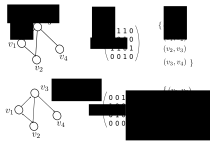
\includegraphics[width=0.7\linewidth]{chapter1/directed_graph.pdf} 
	\caption[Graph, matrix and edge list representations.]{a) Graph representation of undirected (top panel) and directed (bottom panel) network. The same networks are represented with adjacency matrices in column b) and edge list representation in column c).}
	\label{fig:graph_dir}
\end{figure}

The number of edges and nodes are dependent variables. Considering that each node can make $N-1$ connections, the maximum number of the edges in the network is $L_{max}=N(N-1)/2$, as each edge is counted twice. For a directed network, it is possible to draw $L_{max}=N(N-1)$ edges \cite{caldarelli2007scalefree}. When it comes to large networks, they are sparse, meaning that the number of links is $L<<L_{max}$. Consequently, the adjacency matrix is also a sparse structure (has many zeros) that takes a large portion of computer memory \cite{barabasi2016network}. 
It is common to represent the graph as an edge list. In this case, illustrated in Figure \ref{fig:graph_dir}, column c), a graph is described with the list of links that are in the graph, $G = \{ \{v_i,v_j\}\}$. Still, with this representation, we cannot distinguish between directed and undirected graph structures, so the computational algorithm should specify if the edges are symmetric or not.  

Sometimes is essential to include the specific properties of the system in the network representation. For example, to emphasize the frequent interactions between nodes, edges can be assigned with different values; such networks are \textbf{weighted}. In a collaboration network, authors who collaborate more often have stronger interaction. They can be described with an adjacency matrix, whose elements can take any real number $A_{ij}=w_{ij}$ and $w_{ij}>0$. In general, edges may be associated with any categorical variable. Similarly, properties can be added to nodes or the whole network structure. Edges could be characterized by the time when the interaction between nodes happens, which includes the \textbf{temporal} component in the network representation, as in phone calls networks. Finally, if two nodes interact differently, the \textbf{multigraph} is an appropriate configuration where multiple edges are allowed. The transportation network, consisting of roads and railways, could be seen as a multigraph. Figure \ref{fig:multigraph} presents the graphical representation of discussed network representations.


\begin{figure}[h]
	\centering
	\includegraphics[width=0.4\linewidth]{chapter1/multi_graph.pdf} 
	\caption[Different network representations.]{The complex networks may represent different system characteristics. The edges can be directed, weighted or multiply. Also, nodes can be assigned with different weights or any relevant feature.}
	\label{fig:multigraph}
\end{figure}

A \textbf{bipartite network} consists of two types of nodes. The nodes in the same partition are not connected, while links exist only between partitions, Figure \ref{fig:bipartite}. For many real systems, a bipartite graph is a natural representation \cite{barabasi2016network, latora2017complex}. For example, the bipartite network of people and groups has two distinct node partitions, where links indicate the memberships. Another example is a system of customers and products. The user and item link is created when the user bought an item. The bipartite networks find their application in the algorithms for recommender systems, whose goal is to suggest items that may interest the user. They are often used to find the most probable missing links in the network. 

Though the nodes in the same partition of a bipartite network are not directly connected,  we can analyze their connections by projecting the bipartite network to one partition. The primary assumption is that two nodes in one partition could be connected if they point to the same node in the other partition. Figure \ref{fig:bipartite} shows two projections of the bipartite networks. Consider the network of movies and actors. The one-mode projection of movies is an undirected network whose links indicate that two movies share the same actors. On the other hand, another projection is a network of actors. The links exist if two actors appear in the same movie \cite{newman2010, barabasi2016network}.

\begin{figure}[h]
	\centering
	\includegraphics[width=0.7\linewidth]{chapter1/bipartite_graph.pdf} 
	\caption[Bipartite network.]{Bipartite network and two partition projections.}
	\label{fig:bipartite}
\end{figure}

We should be aware that important information is lost when creating a one-mode projection. First, having weighted edges in the network of actors is necessary to know in how many movies two actors appear. From the one-mode projection, we can not reconstruct the original network. Moreover, two different bipartite networks may have the same projected networks. The important consequence of the network projection is the creation of cliques, i.e., subgraphs where all nodes are connected. \\
In general, it is possible to define the k-partite network. The same rules apply as before. There are $k$ distinct node partitions, while the edges exist only between different types of nodes.

\textbf{Temporal networks.}
Studying real systems as static networks can give us a lot of insight into the system's properties. Still, real systems are not static; they evolve not only in the number of elements but also in the number of interactions between them. Some interactions in the system may repeat in different intervals and could be described with complex activity patterns. Including time dimension in the network representation allows us to study the properties of the system closely. The temporal information may matter a lot \cite{holme2012}. For example, if the interaction between nodes $(v_1, v_2)$ happened before in time than  $(v_2, v_3)$, then nodes $v_1, v_3$ might not be connected, as is the case in the static network. 

The temporal network is a collection of timestamped edges; as seen on Figure \ref{fig:temporal} - top panel. Each edge is defined as $(v_i, v_j, t, \Delta t)$, where $v_i$ and $v_j$, are nodes $t$ is time when interaction happen, and $\Delta t$ is event duration \cite{guide_temporal}. The duration of the events may vary, as in the phone-call network. Also, for many systems, the time resolution of the event duration is too small. For example, this parameter may be neglected when people interact on social platforms or email each other because the event time is too short; it scales in seconds.

\begin{figure}[h]
	\centering
	\includegraphics[width=0.7\linewidth]{chapter1/temporal_network.pdf} 
	\caption[Temporal network.]{Top panel represents temporal network as collection of timestamped edges. Bottom panel represents sequence of static networks.}
	\label{fig:temporal}
\end{figure}

The temporal network can be represented as a sequence of static networks that evolve in time, $G = \{ G(t_1), G(t_2), ..., G(t_{max})\}$, as shown in Figure \ref{fig:temporal} - bottom panel. At each time step, we can create the network and analyze the macroscopic properties of the given network snapshot. With this, we can end up with graph snapshots with many disconnected components or empty graphs for some points \cite{holme2015modern}. Sometimes, a better approach is aggregating the links over time windows. Here, we need to specify the time window length $w$. Interactions in the time interval $0\leq t<w$ enter the first snapshot. The following snapshot takes edges $w \leq t <2w$, and so on. The time windows are not overlapping, but generally, it is possible to slide the time window for different periods $ 1 \leq \delta t < w$. The downside of this method is that we can not recover original data points. The larger the time window is, the more information is lost. If the time window is set to $w=t_{max}$, there is only one snapshot, and the temporal data are no more available \cite{krings2012effects, arnold2021moving}. 

\textbf{Multilayer networks} were introduced for studying systems in which different types of interaction exist. This formalism allows one to investigate diverse network systems and combine different data types into one model \cite{porter2018multilayer}. In a multilayer or multiplex network, all nodes are present in each layer, but their interactions among layers differ. Two nodes may be connected in one layer but not in the other. Different online social systems may be an example of a multiplex network when users are connected on one platform but not on the other \cite{aleta2019multilayer}. Another example is the airline transportation network, where each layer represents the flights of different airline companies \cite{kivelamultilayer}.  


\section{Thesis outline}

This thesis uses combined approaches of statistical physics and complex network theory to model and analyze evolving online social systems. These systems consist of many users interacting online and could be represented by complex networks. The main focus of the thesis is to explore the evolution of these complex networks and understand how different dynamical processes shape their structure. We study the growth of various online social networks using data from Meetup, Reddit, and StackExchange platforms and detect important structural changes in these systems, as well as the processes that lead to the creation of groups and factors important for the emergence of sustainable communities.

In chapter \ref{Ch:Method}, we provide the methodology employed for this research. We describe the fundamental measures of complex networks and introduce basic complex network models. We review the most common probability distributions characterizing complex systems' properties and outline distribution fitting methods. Finally, we introduce the multifractality of the time series and dynamical reputation model. 

Chapter \ref{Ch:signals} addresses the difference between network models where the growth in the number of nodes is constant and when it follows a non-trivial growth signal. This research aims to quantify how growth signals influence the structure of complex networks. Using the adapted aging model \cite{hajra2004}, we use computer simulations to generate different kinds of complex networks. For more realistic real-world network simulations, growing signals are time series of new users from online social platforms, MySpace, and Tech group from Meetup. They are described with trends, cycles, and long-range correlations. Often time series have multi-fractal properties. The results of this study are published in \cite{vranic2021growth}, and they show the importance of growth signals in shaping the network structure because the scale-free networks, which represent real systems, are mainly altered. 

As research on social groups mainly focuses on a single group, there are remaining questions about the characteristics of the entire system. For example, the Tech group is only one of the groups around which Meetup users organize; many other groups are created worldwide, so the system constantly grows. In chapter \ref{Ch:Groups}, we will examine how groups on online social platforms grow. The results are summarised in the paper  \cite{vranic2022universal}. This research is based on Reddit and Meetup data. From Meetup, we created two data sets, one with groups created in London and the other with groups created in New York, while for Reddit, we selected groups built before 2012. We are interested in explaining scaling behavior in group size and growth rate distributions and identifying the growth mechanisms present in the system. Using a bipartite complex network model, we can reproduce the universality found in the system.

Even though across complex systems, we find the emergence of universal behavior, for example, the scaling of the degree distribution of two groups is similar, different factors might influence its success. It is well known that many online groups may suddenly fall apart. These questions are the subject of the chapter \ref{Ch:Trust}, which main results are published in the paper \cite{vranic2022sustainability}. Here, we study the question-answer platform Stack Exchange; it has more than 200 different topic-specific sites where people help each other answer questions. What is interesting about this system is that some sites were closed because they did not produce enough activity. For that reason, we selected the sites with the same topic that failed, but later, when someone proposed the site again, it stayed active. We analyze the evolution of user interaction networks; here, we use the temporal network approach and compare active and closed sites. We find that it is essential how the network users are distributed into a core-periphery structure \cite{gallagher2020clarified}. The core must select firmly connected users, but their interaction with the periphery has to be high. In other words, a trustworthy core is needed to hold the community. Introducing the Dynamical Reputation Model (DIBRM) \cite{melnikov2018toward}, based on user interaction sequences, we quantify how much users can be trusted and whether a community has a strong core. We briefly describe the Stack Exchange sites in the appendix \ref{App:SE}. In appendix \ref{App:parameters} and \ref{App:sliding} discuss how we choose parameters for the DIBRM model, while in appendix \ref{App:robust} we discuss the stability of inferred core-periphery structures. 

Finally, in chapter \ref{Ch:Conclussion}, we draw the main findings of this thesis. 

\selectlanguage{english}















\chapter{Methodology} % Main chapter title

\section{Complex networks}

Many real systems are composed of a large number of elements interacting with each other. Due to interactions, without any central force, the system exhibits the emergence of collective behaviour on the macro level. Such a system is called a Complex System and its properties can not be predicted from the behaviour of the one individual. An example of a complex system is the human brain. The structure of the brain network and its properties are fundamental for brain functioning, while an emergent phenomenon is a human intelligence. In societies, people's interactions lead to civilization, economy, formation of social groups. Also, the animal populations show different levels of organization that emerge from the individual's interactions \cite{boccaletti2006complex}. %latorro

The research in complex systems focuses on the structure of the interactions between units. Knowing how branches of the system are connected, we can determine the emergence of the collective behaviour of the system. For the brain network, we can construct representation with neurons and synapses, representing the brain connectivity. Neurons in the same brain area are closely connected \cite{latora2017complex}. Similarly, we can define communication between people. The structure of these interactions gives us insights, for example, how information propagates through the system. The presence of people with many connections can lead to faster information flow. 

Despite the differences between complex systems, they can be studied using complex networks; with sets of nodes (vertices) and links (edges). Elements in the system are nodes, while interactions between them are given as edges. This approximation allows us to treat equally social (graph of actors), biological (network of proteins) or even technological systems (internet, traffic) \cite{costa2007characterization, costa2011analyzing}.  In recent years, complex network theory has application in different fields, and the availability of big data incurs its development.
%Analyzing and Modeling Real-World Phenomena with Complex Networks: A Survey of Applications
%Characterization of Complex Networks: A Survey of measurements

The complex network theory originates from the graph theory in mathematics. %These days, the graph and network are used as equivalent terms. 
The first mathematical problem solved using graph theory was $Konigsberg$ problem of seven bridges. The city $Konigsberg$ had seven bridges connecting the city's parts across the river and the island in the middle. The question was, is it possible to find a walk that crosses all seven bridges only once. Representing the problem as a graph, as in figure \ref{fig:Krgraph}, Euler managed to simplify the problem; the parts of the land are represented as nodes while bridges between them are links. Crossing each bridge only once is possible if each part of the land has an even number of connections. By this it is possible to enter one part of the land from one bridge and leave it by the other. As each node has odd number of connections, in this case it is not possible, see Fig. \ref{fig:Krgraph}.

\begin{figure}[!ht]
	\centering
	\includegraphics[width=0.3\linewidth]{Figures/Konigsberg_bridges.png} \hspace{2cm}
	\includegraphics[width=0.3\linewidth]{Figures/Konigsberg_graph.png}
	\caption{The Kronigsber problem of seven bridges.}
	\label{fig:Krgraph}
\end{figure}

\section{Types of networks}

The graph or network $G$ is defined as $G=(\boldsymbol{V}, \boldsymbol{E})$, where $\boldsymbol{V} = \{ v_1, v_2, ... v_N\}$ is a set of $N$ nodes (vertices), and  $\boldsymbol{E} = \{e_1, .. e_L\}$ is a set of $L$ edges (links). The edge is pair of nodes $e = (v_i, v_j), $ such that $\{v_i,v_j\}\in \boldsymbol{V}$. The most basic network representation considers \textbf{unweighted and undirected} structure. The edges are unweighted, meaning that all interactions in the network are equally important.  Because network is un-directed, edges are symmetric, such that $(v_i, v_j)$ implies $(v_j, v_i)$. In \textbf{directed} networks this simmetry is broken. The interaction between two nodes $v_i$ and $v_j$, can be only in one direction. A typical example is World Wide Web, where webpages are nodes and hyperlinks are directed edges. In biological networks, gene regulation and neural activation can be described as directed network. The first column a) in Figure \ref{fig:graph_dir} shows the graphical representation of two networks with equal number of nodes; the first one is underected and the second one is directed. 

Even though, graphical representation can be useful for describing the network structure, mathematical representation allow us to characterize the statistical properties of the networks. The graph $G$, with $N$ nodes could be represented with \textbf{adjacency matrix} $|A| = N \times N$ \cite{boccaletti2006complex}. The elements of the matrix are positive if there is connection between two nodes $v_i$ and $v_j$. 
\begin{equation}
A_{ij} =
\begin{cases}
1 & \text{ ($v_i$, $v_j$) $\in$ $E$}\\
0 & \text{ ($v_i$, $v_j$) $\notin$ $E$}
\end{cases}       
\end{equation}

The column b) on Figure \ref{fig:graph_dir} shows adjacancy matrix representation of given graphs. By convention diagonal elements $A_{ii}=0$, as self-loops are not allowed. For undirected network adjacency matrix is symmetric $A_{i,j}=A_{ji}$, but in the case of directed network matrix is not symmetric, as edges are drawn in one direction only.  

\begin{figure}[H]
\centering
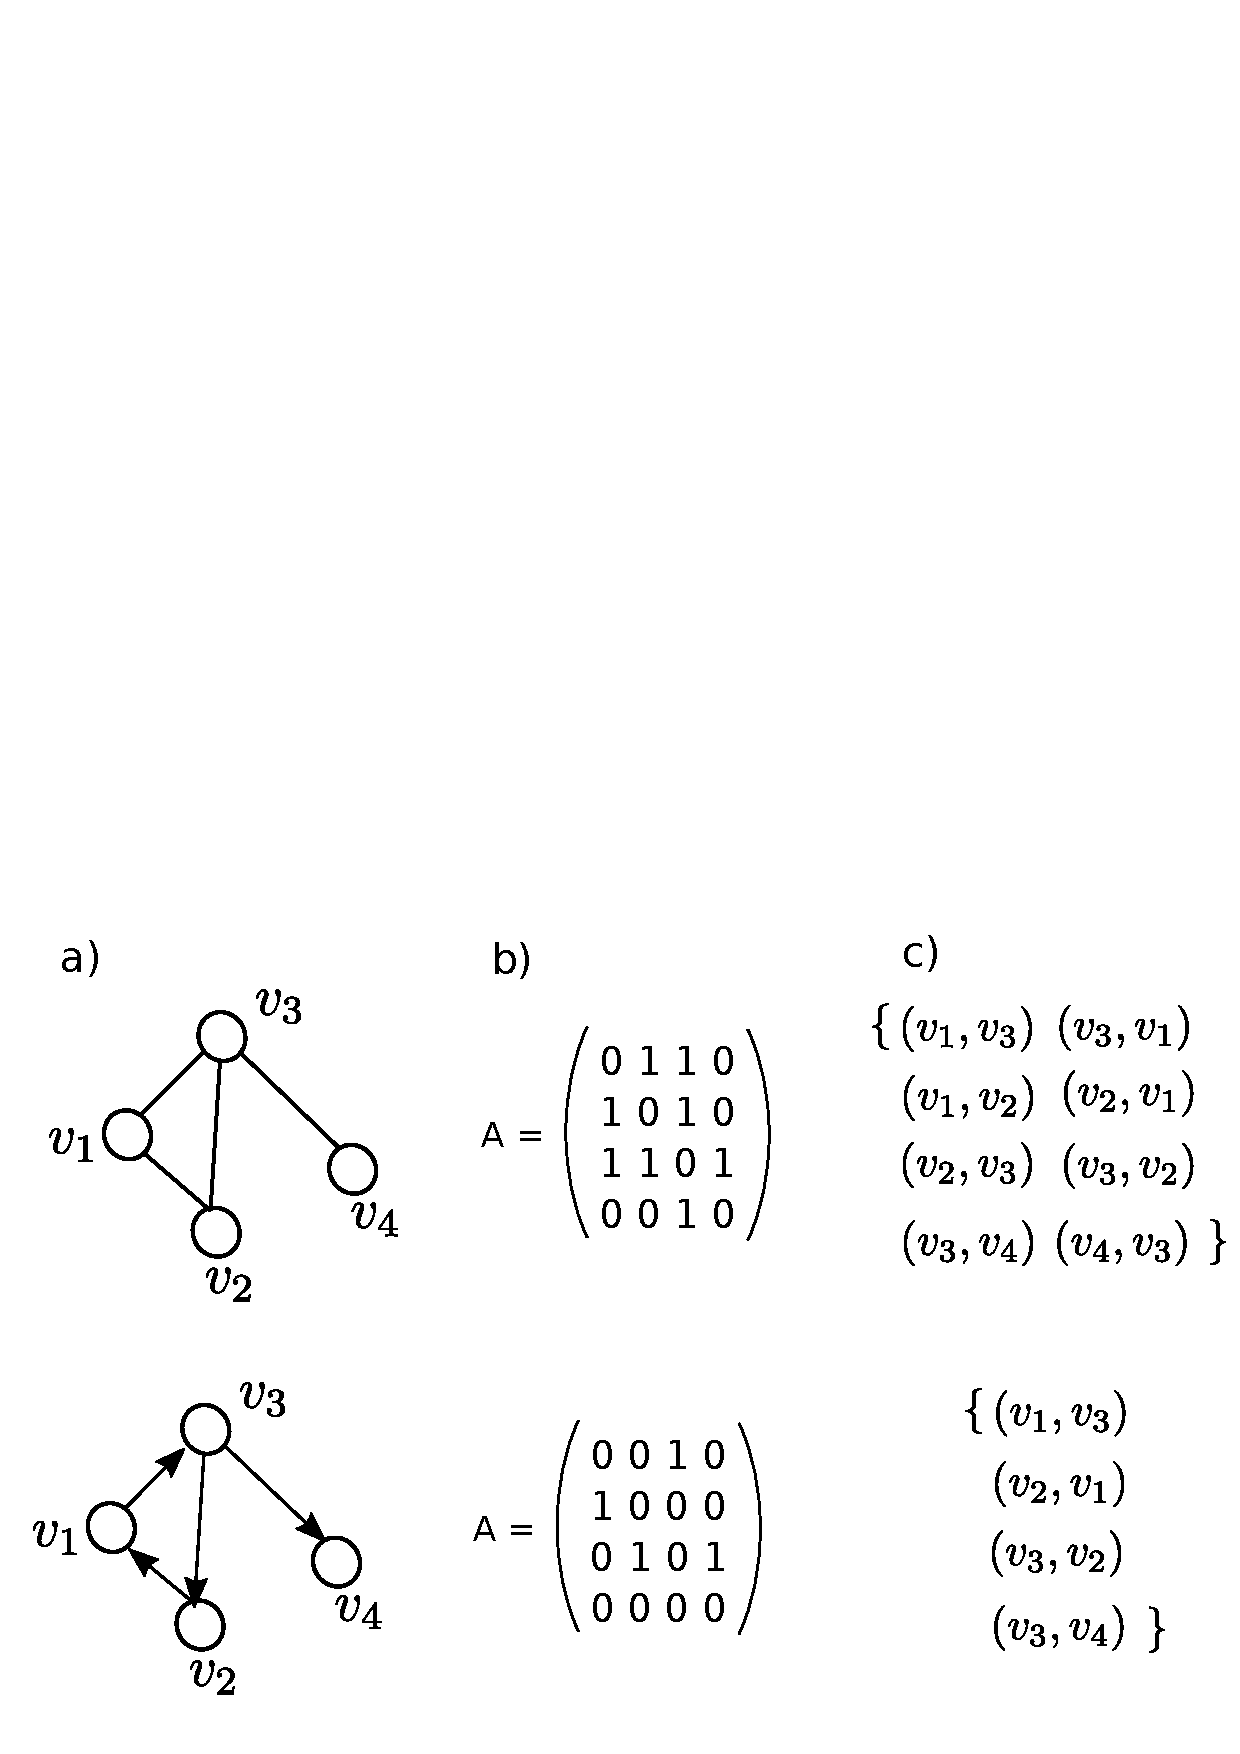
\includegraphics[width=0.7\linewidth]{figures/methodology/directed_graph.pdf} 
\caption{a) Graph representation of undirected (top panel) and directed (bottom panel) network. The same networks are represented with adjacency matrices column b), and edge list representation in column c).}
\label{fig:graph_dir}
\end{figure}

The number of edges and nodes are dependent variables. Considering that each node can make $N-1$ connections, the maximum number of the edges in the network is $L_{max}=N(N-1)/2$, as each edge is counted twice. For directed network it is possible to draw $L_{max}=N(N-1)$ edges \cite{caldarelli2007scalefree}. When it comes to large networks, they are sparse, meaning that the number of links is $L<<L_{max}$. As consequence, the adjacency matrix is also sparse structure (has many zeros) that takes large portion of computer memory \cite{barabasi2016network}. 
It is common to represent the graph as edge list. In this case, illustrated on Figure \ref{fig:graph_dir}, column c), graph is described with the list of links that are in the graph, $G = \{ \{v_i,v_j\}\}$. Still with this representation we are not able to distinguish between directed and undirected graph structures, so in the computational algorithm should be specified if the edges are considered symetric or not.  
%To distinguish between undirected and directed structures, for undirected representation it is possible writing two edges $(v_i, v_j)$ and $(v_j, v_i)$, otherwise in the computational algorithm should be specified if the edges are considered symmetric or not.

\begin{figure}[H]
	\centering
	\includegraphics[width=0.4\linewidth]{figures/methodology/multi_graph.pdf} 
	\caption{The complex networks may represent different characteristics of the system. The edges can be directed, weighted or multiply. Also nodes can be assigned with different weights or any relevant feature.}
	\label{fig:multigraph}
\end{figure}

To create the more realistic models, sometimes is essential to include the specific properties of the system in the network representation. For example, to emphasis the frequent interactions between nodes, edges can be assigned with different values, such networks are \textbf{weighted}. They can be described with adjacency matrix, whose elements can take any real number $A_{ij}=w_{ij}$ and $w_{ij}>0$. In general edges may be associated with any categorical variable. Similarly additional properties can be added to nodes, or even to the whole network structure. To include the \textbf{temporal} component in the network, edges are characterized with the time when the interaction between nodes happen. Finally, if two nodes interact in different ways, the \textbf{multigraph} is appropriate configuration where multiply edges are allowed. The graphical representation of discussed network representations is given on the Figure \ref{fig:multigraph}.

% the network between cities, edges may be different driving paths between them. In neuron cells, multiply synapses are represented as distinct edges. \\ %\cite{barabasi2016network, latora2017complex, newman2010}
A \textbf{bipartite network} consists of two types nodes. The nodes in the same partition are not connected, while links exist only between partitions. For many real systems, a bipartite graph is a natural representation\cite{barabasi2016network, latora2017complex}. For example, the bipartite network of people and groups has two distinct node partitions while links indicate the memberships. Another example is a system of customers and products. The link between user and item is created when the user buys an item. The bipartite networks find their application in the algorithms for recommended systems, whose goal is to recommend items that may interest the user. Actually, to find the most probable missing links in the network. 

In a bipartite network, nodes in one partition are not connected. Still, we can analyse a single node type if we project the bipartite network on one partition. The primary assumption is that two nodes in one partition could be connected if they point to the same node in another partition. Consider the network of movies and actors. The one mode projection of movies is an undirected network whose links indicate that two movies share the same actors. On the other hand, another projection is a network of actors. The links exist if two actors appear in the same movie \cite{newman2010, barabasi2016network}.

\begin{figure}[H]
	\centering
	\includegraphics[width=0.7\linewidth]{figures/methodology/bipartite_graph.pdf} 
	\caption{Bipartite graph and two partition projections.}
	\label{fig:gt2}
\end{figure}

We should be aware that important information is lost when creating a one-mode projection. First of all, without having weighted edges in the network of actors, it is impossible to have information on how many movies two actors appear in. From the one-mode projection, we can not reconstruct the original network. Moreover, two different bipartite networks may have the same projected networks. The important consequence of the network projection is the creation of cliques; subgraphs where all nodes are connected. \\
In general, it is possible to define the k-bipartite network. The same rules apply as before. There are $k$ distinct node partitions, while the edges exist only between different types of nodes.



%The product $B_{ki}$ and $B_{kj}$ is 1 if $i$ and $j$ belong to the same group $k$. Thus the total number of groups to which nodes $i$ and $j$ belong is $P_{ij} = \sum_{k=1}^g B_{ki}B_{kj} = \sum_{k=1}^g B_{ik}^TB_{kj}$. The matrix $P$ is matrix of one-mode projection. The diagonal elements are non-zero, and represent the number of groups node $i$ belongs to.  To derive the weighted adjacency matrix, the diagonal elements are set to 0. The adjacency matrix of unweighted projection, each non-zero element needs to be replaced with $1$. 

\textbf{Temporal networks.}
Studying the real systems as static networks can give us a lot of insight into the system properties. Still, real systems are not static; they evolve not only in the number of elements but also in the number of interactions between them. Some interactions in the system may repeat in different intervals and could be described with complex activity patterns. Including time dimension in the network representation allows us to study the properties of the system closely. The temporal information may matter a lot \cite{holme2012}. For example if interaction between nodes $(v_1, v_2)$ happened before in time than  $(v_2, v_3)$, then nodes $v_1, v_3$ would not be connected, as it is the case in the static network. 

The temporal network is a collection of timestamped edges. Each edge is defined as $(v_i, v_j, t, \Delta t)$, where $v_i$ and $v_j$, are nodes $t$ is time when interaction happen, and $\Delta t$ is event duration \cite{guide_temporal}. The duration of the events may vary, as in the phone-call network. Also, for many systems, the time resolution of event duration is too small. For example, this parameter may be neglected when people interact on social platforms or email each other because the event time is too short, it scales in seconds.

\begin{figure}[H]
	\centering
	\includegraphics[width=0.7\linewidth]{figures/methodology/temporal_network.pdf} 
	\caption{Temporal network. }
	\label{fig:gt3}
\end{figure}

The temporal network can be represented as sequence of static networks that evolve in time, $G = \{ G(t_1), G(t_2), ..., G(t_{max})\}$. At each time step, we can create the network and analyze the macroscopic properties of the given network snapshot. With this, we can end up with graph snapshots with many disconnected components or empty graphs for some points \cite{holme2015modern}. Sometimes, a much better approach is to aggregate the links that over time-windows. Here, we need to specify the time window length $w$. Interactions in the time interval $0\leq t<w$ enter the first snapshot. The next snapshot takes edges $w \leq t <2w$, and so on. The time windows are not overlapping, but generally, it is possible to slide the time window for different periods $ 1 \leq \delta t \geq w$. The downside of this method is that we can not recover original data points. The larger the time window is, the more information is lost. If the time window is set to $w=t_{max}$, there is only one snapshot, and the temporal data are no more available \cite{krings2012effects, arnold2021moving}. 

\textbf{Multilayer networks} were introduced for studying systems in which different types of interaction exist. This formalism allows one to investigate diverse network systems and to combine different types of data into one model \cite{porter2018multilayer}. In a multilayer or multiplex network, all nodes are present in each layer, but their interactions among layers differ. Two nodes may be connected in one layer but not in the other. Different online social systems may be an example of a multiplex network when users are connected on one platform but not on the other \cite{aleta2019multilayer}. Or the airline transportation network, where each layer represents the flights of different airline companies \cite{kivelamultilayer}.   

%Consequently, we can partition the set of links into intralayer links, that is, links that connect nodes set in the same layer, and interlayer or coupling links, which are those links that connect nodes set in different layers. 

%A temporal network is a special kind of multiplex network, where these layers form a temporal (ordered) sequence. Crucially, there can dynamics on each vertex that govern which layer some kind of interaction occurs on, so multiplex networks are not merely a special kind of graph in which different colors or layer numbers annotate edges. %clauset preformulisati


%Spatial networks are a special kind of node-annotated network, in which the annotations represent the node's location in some d-dimensional space. This graph property is most common in transportation networks, e.g., as road and city networks, airport transportation networks, oil and gas distribution networks, shipping networks, etc., but can also appear in social networks. Planar graphs are a special case of spatial networks in which the nodes are embedded on a 2-dimensional surface and edges do not cross. %clauset preformulisati

%Hypergraphs are another type of network, in which edges denote the interaction of more than two vertices, e.g, E in V × V × V . Scientific collaboration graphs can be represented as a hypergraph, in which each "edge" is the set of coauthors on a scientific article. However, collaboration networks are more commonly represented as bipartite graphs, in which scientists and papers form two sets of vertices, and scientist-nodes are connected to all the paper-nodes on which they are authors. %clauset to do

%The canonical network form is an undirected graph, where two nodes are either connected or not. This applies to situations where two nodes are either in a relationship with each other or not, but it cannot be that one is related to the second without the second being related to the …rst. This is generally true of many social and/or economic relationships, such as partnerships, friendships, alliances, acquaintances, etc. This sort of network will be central to most of the chapters that follow. However, there are other situations that we will examine that are better modeled as directed networks, where one node may be connected to a second without the second being connected to the …rst. For instance, a network that keeps track of which authors cite which other authors, or which web pages have links to which others would naturally take the form  of a directed graph.

\section{The structure of complex networks}

%The complex system can be represented by complex network $G=(V, E)$, where the elements of system (atoms, proteins, people) map to set of $N$ nodes $V=\{1, 2, ...,N\}$. The interactions between elements map to $L$ links between nodes, $E = \{ e_1, e_2... e_L\}$. The \textbf{adjacency matrix} ${A} = N \times N$ has value $1$ if there is connection between two nodes, otherwise it is $0$ \cite{boccaletti2006}. 

\subsection{Degree distribution}

The simplest network measure is \textbf{node degree}, $k$. The degree of node $i$ gives the number of nodes attached to node $i$, $k_i = \sum_j A_{ij}$. The density of the network is average degree divided by $N-1$, where $N$ is number of nodes. It is relative fraction of nodes in the network. 

In the case of regular networks, such as grids, each node has an equal degree, meaning that nodes in the network have similar roles. In the general case, the networks have more complicated structure. If degree sequence is skewed, we are able to identify nodes with high degree, hubs. Removing hubs may partition a connected network into several components. Finally, if we are able to test isomorphism between two graphs, the starting point would be to compare their degree sequences are the same. If they are not same, then graphs can not be isomorphic.

To calculate the degree distribution we can consider the fraction of $k$ degree nodes $N_k$, $p(k) = N_k/N$. It is the probability , $P(k)$, that randomly chosen node has degree $k$. Similarly, we can order nodes according to their degree and plot the node degree.

%\begin{figure}[h!]
%	\centering
%	\includegraphics[width=0.7\textwidth]{codes/test1.pdf}
%	%figures/methodology/distributions.png}
%	\caption{Distributions on linear and logarithmic scale.}
%	\label{fig:dist}
%\end{figure}

%If degree distribution is present $P(k)$, and the total number of nodes is fixed to $N$. We can construct a graph with random connections. Label N vertices. To node $j$ of the graph ascribe degrees $k_j$, taken from the distribution $P(k)$. Connect at random ends of pairs of distinct quills belonging to distinct vertices. 

If the nodes of the graph are statistically independent, the degree distribution completely determines the properties of a network. Here we summarize the forms of degree distributions that are mostly found in the complex network theory:
\begin{itemize}
	\item The Poisson distribution. The degree distribution in random network, where all nodes have the same connecting probability, follows Poisson distribution $P(k)= \frac{(Np)^ke^{-Np}}{k!}$, where $k$ is the mean degree distribution. 
	
	\item Exponential distribution. $P(k) = e^{-k/ \- k}$. This is degree distribution of the growing random graph. Even for infinite networks all moments of distributions are finite, and have natural scale of the order of average degree.
	
	\item In many real networks degree distribution follows a power law. $P(k) = k ^ {-\gamma} $, where $\gamma$ is exponent of the distribution. In this distribution there is no natural scale, so they are called scale-free networks. In infinite networks all higher moments diverge. If the average degree of scale-free networks is finite, than $\gamma$ exponent should be $\gamma>2$. Therefore, real networks have a scale-free structure with the emergence of the hubs \cite{newman2010}. 
	%In finite size networks, fat-tailed degree distributions have natural cut-offs. 
\end{itemize}

When plotting the degree distribution, it is common to use scaling of the axis. As many nodes have  low degree, like for power-law or exponential distribution it is more useful to use logarithmic scale. Now it is more easily notices that data-points follow straight line, meaning that degree distribution is some kind of exponential function. 

%On the logarithmic scale the distance between two points is proportional to the logarithm of distance between two points, meaning that distance on logarithm scale is same between points 10 and 100, and 100 and 1000.  

\subsection{Degree correlations}

Correlation is defined through a correlation coefficient r. If x and y are two stochastic variables, for which we have a series of observation pairs $(x_1, y_1), (x_2, y_2), ... (x_n, y_n)$. The correlation coefficient $r(x, y)$ between $x$ and $y$ is defined as:

\begin{equation}
r(x, y) = \frac{\frac{1}{n}\sum_{i=1}^{n}((x_i - \bar{x} ) (y_i - \bar{y}) )}{\sqrt{\frac{1}{n}\sum_{i=1}^{n}(x_i - \bar{x})^2} \sqrt{\frac{1}{n}\sum_{i=1}^{n}(y_i - \bar{y})^2} }
\end{equation}

where $\bar{x} = \frac{1}{n}\sum_{i=1}^{n}x_i$, is the average over variable $x$.

Taking the definition of correlation coefficient we can define it for vertex degrees. For simple graph G with vertex set $V(G) = \{v_1, ..v_n\}$, $\boldsymbol{A}[i,j] = 1$ if there is a link between nodes $v_i$ and $v_j$. If G is a simple graph with adjacency matrix $\boldsymbol{A}$ and degree sequence $\boldsymbol{d} = [d_1, ..., d_n]$

\begin{equation}
r_{deg}(G) = \frac{\sum_{i=1}^{n}\sum_{i=1+1}^{n}((d_i - \bar{d}) (d_i - \bar{d}) \boldsymbol{A}[i,j] )}{\sum_{i=1}^{n}(d_i - \bar{d})^2}
\end{equation}

Using adjacency matrix, allow us to calculate the correlations between neighboring nodes. If two nodes are not connected $A[i,j]=0$, the degree correlation between them does not have contribution to the $r$.

The \textbf{degree-degree correlations} in the network are measured by \textbf{assortativity}. If correlations are positive, networks are assortative; there is a tendency that connections exist between similar degree nodes. The negative correlations indicate that large degree nodes have preference to connect nodes with small degree; dissasortative networks. The average first neighbor degree $k_{nn}$ can be calculated as $k_{nn} = \sum_{k^{'}}k^{'}P(k^{'}|{k})$. The $P$ is conditional probability that an edge of degree $k$ points to node with degree $k$. The norm is $\sum_{k^{'}}P(k^{'}|k)=1$, and detailed balance conditions \cite{boccaletti2006complex},  $kP(k^{'}|k)P(k) = k^{'}P(k|k^{'})P(k^{'})$ \cite{boccaletti2006complex}. If the node degrees are uncorrelated, $k_{nn}$ does not depend on the degree, otherwise increasing/decreasing function indicates on positive/negative correlations in the network.

The Newman defined the assortativity index $r$ in slightly different way:

\begin{equation}
r = \sum_{kl}kl(e_{kl} - q_lq_k) / \sigma_q^2
\end{equation}

where $e_{kl}$ is the probability that randomly selected link connect nodes with degrees $k$ and $l$, $q_k$ is probability that randomly choosen node is connected to node $k$ and equals $q_k = kp_k / \langle k \rangle$, while $\sigma_q$ is variance of the distribution $q_k$. 

\subsection{Clustering coefficient}



%A common way toward spreading information is simply having a node update its neighbors. In turn, neighbors can inform their neighbors, and so on. There are many variations to this model, such as having a node select only one or a few of its neighbors, or deciding to stop spreading updates when it notices that a selected neighbor already has the information. Informally, this type of dissemination is often described in the form of gossiping models, also known as epidemic dissemination [Eugster et al., 2004]. The model is very general: instead of information we can also consider spreading of diseases, but also viruses over the Internet. Another example is that of forming of opinions, which often depends on what the majority of your community thinks. We shall return to these issues in more detail when discussing peer- to-peer networks in Chapter 8.

%When considering real-world networks, we often see that they are organized as a collection of interconnected groups. In terms of social networks, this means that we can often clearly distinguish communities of nodes with many links between its members, yet relatively few links between nodes that belong to different communities. Actually indicating which nodes belong to which communities may not be easy at all. Also, nodes generally belong to more than one community. However, we can express the existence of communities by means of a clustering coefficient. As shown by Xu and Liu [2008], it turns out that there is a clear relationship between the speed by which information is disseminated in social networks and the clustering coefficient: the higher the degree of clustering, the slower the dissemination. To a certain extent, this result may seem quite obvious, but from a formal (i.e., mathematical) point of view, it turns out to be not so trivial. What this means is that if we want to design a dissemination protocol, we may need to take special measures in highly clustered networks in order to guarantee a certain performance regarding the dissemination speed. This alone has been enough reason for researchers to define and measure the clustering coefficient of a network. Besides this reason, measuring the clustering coefficient obviously alows us to simply compare different networks, without necessarily wanting to make use of the actual values of the respective coefficients. In this sense, clustering coefficients can help in classifying networks.

The \textbf{clustering coefficient} is a measure describing the neighbourhood's structure. In networks exist tendency to form triangles or clusters. This is common in friendship networks where two friends of one person have a high probability of being friends. The clustering can be measured by computing the number of links between neighbours of one node,
\begin{equation}
c_i=2e_i/(k_i(k_i-1))
\end{equation}

Averaging it over all network nodes, we can calculate the mean clustering coefficient. It ranges from  $\langle c \rangle = 0$ where connections between neighbouring nodes do not exist, network has the structure of three. On the other hand, $\langle c \rangle = 1$ indicates a fully connected network. 

Newman proposed the alternative definition for the clustering coefficient based on the number of triples and triangles in a graph. A triangle at node $v$ is complete subgraph with 3 nodes, including $v$. A triple on the node v is a subgraph of exactly three nodes and two edges, where v is incident with two edges. The network transitivity is defined as the ratio of number of triangles in the network over the number of triples. The network transitivity is seen as global clustering, as it considers the whole network.  


%n the network literature we ocassionally encounter the global cluster- ing coefficient, which measures the total number of closed triangles in a network. Indeed, L i in (2.15) is the number of triangles that node i partic-ipates in, as each link between two neighbors of node i closes a triangle (Figure 2.17). Hence the degree of a network’s global clustering can be also captured by the global clustering coefficient, defined as 

%where a connected triplet is an ordered set of three nodes ABC such that A connects to B and B connects to C. For example, an A, B, C triangle is made of three triplets, ABC, BCA and CAB. In contrast a chain of connected nodes A, B, C, in which B connects to A and C, but A does not link to C, forms a single open triplet ABC. The factor three in the numerator of (2.17) is due to the fact that each triangle is counted three times in the triplet count. The roots of the global clustering coefficient go back to the social network literature of the 1940s [17, 18], where C Δ is often called the ratio of transitive triplets.

\subsection{Network paths}
In the network structure, the interacting nodes are directly connected with the edge. In this representation we can say that distance between them is $d_{v_i, v_j}=1$. Distance defined like this does not have any physical meaning. Its purpose is to describe how the position of nodes in the network structure influences the other distant nodes. 

The \textbf{path} between two nodes, $v_i$ and $v_j$ is a sequence of edges $\{(v_1, v_2),  (v_2, v_3), ...(v_k, v_{k+1})\\,... (v_{n-1}, v_n)\}$, where $v_1=v_i$, $v_n=v_j$. In the path, the nodes are distinct. Otherwise, the sequence is called a \textbf{walk}, where each node can be visited many times. Also, it is possible to define a \textbf{cycle}, a path that starts and ends on the same node while other nodes in the cycle are distinct. The length of the path, walk or cycle is the number of links in the sequence. Using the adjacency matrix we can easily calculate the number of walks between two nodes. The $A^2$ gives us walks of length $2$, the $A^3$, number of walks of length 3, and so on. 

The network is connected if it is possible to define the path between every two nodes in the network. When it is not the case, the network is disconnected into two or more connected components. Note that the component can be an isolated node. Also, in directed networks may happen that node $v_i$ is reachable from node $v_j$, but if we start from $v_j$ we can not find the path to the $v_i$. Such a graph is connected but is called a weakly connected component. 

We can find different paths between two nodes in the network, but the most important one is the \textbf{shortest path}. The distance between two nodes $d(v_i, v_j)$ is defined as the shortest path length between two nodes. 
In the case of weighted networks, it is the path with minimal weight, and the length of such path does not have to be minimal. Distances on the network can give us insight into how similar networks are and indicate the node's relative importance in the network. 

%The node's eccentricity shows how far the farthest vertex is positioned in the network. 
The \textbf{radius} is the minimum overall eccentricity values, while the \textbf{diameter} defines the largest distance between nodes in the network. These definitions apply to directed and undirected graphs. 

If G is a connected graph with vertex set V and $\bar{d}(u)$ is the average length of the shortest paths from node u, to any other node v in network G.

\begin{equation}
\bar{d}(u) = \frac{1}{|V|-1} \sum_{v\in V, v \notin u} d(u,v)  
\end{equation}

From there, the \textbf{average path length} is mean value over $\bar{d}(u)$.

\begin{equation}
\bar{d}(G) = \frac{1}{|V|}\sum_{u \in V} \bar{d}(u)
\end{equation}

while the \textbf{characteristic path} length of G is median over all $\bar{d}(u)$.

%Eulerian tours and Hamiltonian cycles

%A walk is said to be closed if it starts and ends at the same node. It is clear that in
%order to have a closed walk that involves every link of a network exactly once it must
%be that each node in the network has an even degree. 39 This follows since each time a
%node is “entered” by one link on the walk it must be “exited”by a di¤erent link, and
%each time the node is visited, it must be by a link that has not appeared previously on
%the walk. Euler’s [?] simple but remarkable theorem is that this condition is necessary
%and su¢ cient for there to exist such a closed walk.

%A connected network g has a closed walk that involves each link ex-%actly once if and only if the degree of each node is even.


%One can ask a related question for nodes rather than links: when is it possible to
%…nd a closed walk that involves each node in the network exactly once? Such a closed
%walk must be a cycle, and is referred to as a Hamilton Cycle or a Hamiltonian. A
%related question is whether there exists a “Hamilton path”that hits each node exactly
%once. Clearly a network that has a Hamilton cycle has a Hamilton path, while the
%converse is not true (consider a line).
%Discovering whether or not a network has a Hamilton cycle is a much more chal-
%lenging question than whether it has a Euler tour; and this has been an active area
%of research in graph theory for some time. It has direct applications to the “traveling
%salesman problem,”where a salesman must visit each city on a trip exactly once, cities
%are nodes on a network, and the path must follow the links.
%The seminal theorem on Hamilton cycles is due to Dirac [?]. Stronger theorems
%have since been developed, as we shall shortly see, but it is worth stating on its own,
%as it has an intuitive proof that helps one see the paths to proving some of the later.




%The diameter gives us helpful information, it may not be powerful enough to discriminate among graphs. An important metric is considering path length distribution, and the average distance between nodes is helpful for network description.




%There are a few particular network structures that are commonly referred to.
%A tree is a connected network that has no cycles.
%A forest is a network such that each component is a tree. Thus any network that
%has no cycles is a forest, as in the example pictured in Figure 2.1.6.
%A particularly prominent forest network is a star. A star is a network such that
%there exists some node i such that every link in the network involves node i. In this
%case i is referred to as the center of the star.
%There are a few facts about trees that are easy to derive (see Exercise 2.2) and
%worth mentioning.
%A connected network is a tree if and only if it has n
%1 links.
%A tree has at least two leaves, where leaves are nodes that have exactly one link.
%In a tree, there is a unique path between any two nodes.
%The complete network is one where all possible links are present, so one where
%where g ij = 1 for all i 6 = j.



\subsection{D-measure}

%Between two nodes in the network, we can define different paths, but the most important one are the shortest paths, $d_{ij}$. Diameter defines the largest shortest path found in the network. 

For each node $i$ we can define the distribution of the shortest paths between node $i$ and all others nodes in the network, $P_{i}=\{p_{i}(j)\}$, where $p_{i}(j)$ is percent of nodes at distance $j$ from node $i$. The connectivity patterns can efficiently describe difference between two networks.    
To specify how much $G$ and $G^{'}$ are similar we use D-measure \cite{tiago2}
\begin{equation}
D(G, G^{'}) = \omega \left| \sqrt{\frac{J(P_1,..P_N)}{log(d)}}-\sqrt{\frac{J(P_1^{'},..P_N^{'})}{log(d^{'})}} \right| + (1-\omega) \sqrt{\frac{J(\mu_{G},\mu_{G^{'}})}{log2}}
\label{eq:dmeasure}
\end{equation}

D-measure calculates Jensen-Shannon divergence between $N$ shortest path distributions,

\begin{equation}
J(P_1,.., P_N)) = \sum_{i,j}p_i(j)log(\frac{p_i(j)}{\mu_j})
\end{equation}

where  $\mu_j = (\sum_{i=1}^N p_i(j))/N$ is mean shortest path distribution.

%TEMPORAL NETWORKS JENSEN SHANNON AND 

The first term in equation \ref{eq:dmeasure} compares local differences between two networks, and Jensen-Shannon divergence between $N$ shortest path distributions $J(P_{1},...,P_{N})$ is normed with network diameter $d(G)$. The second part determines global differences, computing  ${J(\mu_{G},\mu_{G^{'}})}$ between mean shortest path distributions. 
%We consider equally important local and global properties of the networks, and parameter $\omega$ is set to $0.5$. 
The D-measure ranges from $0$ to $1$. The lower D-measure is, networks are more similar and for D-measure $D = 0$, structures are isomorphic.

%OVDE mozda neka slika d-mere da bude intuitivnije kako radi
%\subsection{Real-world networks}
%Real-world networks share similar properties. The mean distance between nodes is smaller than the number of nodes in the network $l << N$, called small-world phenomena. This cause the fast spread of information or even diseases in the complex systems. In small-world networks number of vertices grow exponentially with distance; thus $l$ increase as $log(n)$ or slower. Logarithmic scaling can be proved from various network models; also, it is observed in real-world complex systems. The clustering coefficient in real-world networks is usually high. Real-world networks have one important feature; power-law degree distribution; such networks are called scale-free networks.

\subsection{Community structure}

Nodes can be organized into groups, called communities. Identifying these hidden blocks can lead to interesting insights into the network. The communities are expected in social networks, as people tend to organize into different groups.  

However, the community detection problem does not give a precise definition of what a community is. A common definition of a community is that it is densely connected subgraph \cite{userguide}, \cite{martin}.  In community detection the number of communities is not predefined. The number of possible communities in the network could be large number and we can not analyse all combinations, so we need algorithms to help us to identify potential communities in the network. 

\textbf{Modularity}. Comparing the link density of the community by the link density obtained for the same group of nodes randomly connected we could conclude if the community corresponds to the dense subgraph or the structure is created completely random. The modularity is function that measures the randomness of the each partition. With modularity we can compare the communities and decide which one is better. 

For the network with $N$ nodes and $L$ links that partitions into $n_c$ communities. Each community has $N_c$ nodes and $L_c$ links. If number of links is larger than the expected number of links between $N_c$ nodes given in the expected node sequence than these nodes may form the community. We calculate the difference between real network connectivity $A_{ij}$ and the expected number of links between nodes if the network is randomly connected, $p_{ij}$. The $p_{ij}$ can be obtained by randomizing the original network, but keeping the expected degree of each node unchanged, so $p_{ij}= \frac{k_ik_j}{2L}$.

\begin{equation}
M_c = \frac{1}{2L}\sum(A_{ij}-p_{ij})
\end{equation}

If modularity is positive, the selected nodes may be community as their connectivity is far from random. If $M_c$ is zero, then the connectivity between nodes is random, and if $M_c$ is negative the nodes do not form the community. 

The same idea can be generalized to the whole network: The modularity of network partitioned into $n_c$ communities is then defined as:
\begin{equation}
M=\sum_{c=1}^{n} [\frac{L_c}{L} - (\frac{k_c}{2L})^2]
\end{equation}

The higher modularity indicates that nodes are partitioned in better communities. When we put all nodes into only one community $M=0$, otherwise if each node is community itself $L_c=0$ and the sum is negative. 

Maximum network modularity indicates the best partions. As there are too many partitions, it is not possible to construct all possible partitions and calculate their modularity. For that we need algorithm that could identify the the best partition. 

The first algorithm that was proposed for modularity optimization was greedy algorithm. First it assign each node to community, and start with N communities. Then, we try to merge each pair of communities and calculate the moddularity difference $\Delta M$. Then indentify the community pair for which the difference is largest and merge those two communities. This is repeated untill all nodes merge into single community. The best partition is one with largest $M$. 

\textbf{Louvain algorithm} is optimization algorithm with better scalability than gready algorithm, so it can operate on very large networks. Initially each node is assigned to different community, and similar as before we calculate the difference in the modularity if we move the community of one of its neighbours. Then we move the node i to the community such that modularity becomes larger. This is applyed to all nodes untill no further improvement could be made. In the second step we create weighter network whose nodes are communities identified during first step. The weight of the link between communities is the sum of the weights between the links in the communities, and the number of links inside the community is given as weighted self-loop. Then the first and secound steps are repeated, until there is no more change in the modularity, otherwise until we find the maximum, optimal modularity. 

\textbf{Core-periphery} structure describes a network whose nodes are divided into two community, densely connected core and less connected periphery. If we consider the average probabilities of edges within each group as $p_{11}$ and $p_{22}$, and between groups $p_{12}$, instead of traditionaly assortative or dissasortative structure we can define core-periphery structure $p_{11}> p_{12} > p_{22}$. In the principle core-periphery structure does not have to be limited to only two groups, and we can define layered, onion, structure. The network can have more cores, that are not directly connected to each other. 

The simple method for finding core-periphery structure is to assume that nodes in core have higher degree in the core than in the periphery. Another simple method is to construct k-cores. K core is group of nodes that each has connection to at least k other members of the group. K-cores form a nested set, and become denser with higher k. The core-periphery structure can be detected optimizing the measure similar to modularity, as defined by Borgatti and Everett. Their goal is to find the division that minimizes the number of edges in the periphery. So they define the score function that is equal to number of edges in the periphery minus the expected number of such edges placed at random. $\rho = \frac{1}{2}\sum_{ij}(A_{ij}-p)g_ig_j$.

The another way to detect core-periphery structure is to use the inference method based on fits to a stochastic block model. In this method we fit observed network to a block model with two groups, such that edge-probabilities have form $p_{11}> p_{12} > p_{22}$.

\textbf{Stochastic Block Model} is model where each node, in given network G,  belongs to one of $B$ blocks. Vector $\theta_i = r$ indicates that node $i$ is in block $r$, while SBM matrix $\{p\}_{BxB}$, specify the probability $p_{rs}$ that nodes from group $r$ are connected to nodes in group $s$. The SBM model is looking for the most probable model that can reproduce a given network G. Probability of having model parameters $\theta, p$ given network $G$ is proportional to likelihood of generating network $G$, prior of SBM matrix and prior on block assignments:

\begin{equation}
P(\theta, p| G) = P(G | \theta , p) P(p) P(\theta) 
\end{equation}

\begin{equation}
P(G | \theta , p) = \prod_{i<j} p_{r_is_j}^{A_{ij}}(1-p_{r_is_j})^{1-A_{ij}}  
\end{equation}

where $A_{ij}$ is number of edges between nodes $i$ and $j$. 

Prior on p is modified for core-periphery model such that $P(p) = 3!I_{0<p_{22}<p_{12}<p_{11}<1}$, while prior on $\theta $ consists of three parts: probability of having $l$ blocks; given the number of layers probability $P(n|l)$ of having groups of sizes ${n_1..n_l}$ and the probability $P(\theta|n)$ of having particular assignments of nodes to blocks. 

For fitting model in the work \cite{gallagher2020clarified} authors use Metropolis-within-Gibbs algorithm.
The likelihood of SBM model increase with number of blocks and model itself does not define optimal number of communities. Inferring minimum description length (MDL)
of the model is one approach to decide which model is more likely.      

%Another type of networks is the bipartite network that has two disjoint sets of nodes. The edges exist only between nodes from different sets. Networks of this class can appear in real-world data, such as users-movies preference, collaboration network for scientists and papers, etc. Application of density-based approach requires to first project bipartite network to one of its partitions and then find communities in that projection. With this, some information is lost. On the other hand, the method that is directly applicable to bipartite networks is Stochastic Block model, from which the models considered in this paper are derived.  

\section{Network models}

\subsection{Random network model}

The random graph model was introduced by mathematicians Paul Erdős and Alfred R\' {e}nyi in 1959. In this model, connections between nodes are chosen randomly, and every link has the same probability of existing. The graph is characterized only by a number of the nodes $N$ and the linking probability $p$, so Erdős-R\' {e}nyi graph is written as $G(n, p)$. 

The creation of ER random network consists of the following steps:
\begin{itemize}
	\item we start with $N$ isolated nodes
	\item between each $N(N-1)/2$ pair of nodes we create link with probability $p$; sampling random number $r \in (0,1)$, we create link if $r \leq p$    
\end{itemize}


\begin{figure}[H]
	\centering
	\includegraphics[width=0.9\linewidth]{figures/methodology/ERgraph}
	\caption{ER graph with $N=100$ nodes and different linking probabilities $p$.}
	\label{fig:erp}
\end{figure}

We should note that this process is stochastic. The networks $G(N, p)$ with the same parameters do not need to have the same structure; i.e. they differ in the number of links. Therefore, the single random graph is only one graph from all the possible realizations in the statistical ensemble. 

Two simple quantities that could be estimated are the average number of links and the average degree. For complete graph with $N$ nodes, number of edges is $N(N-1)/2$. As the probability of drawing every edge is $p$, the \textbf{average number of links} is simply given as 

\begin{equation}
\langle L \rangle = \frac{N(N-1)}{2}p
\end{equation}

From there, we conclude that the network's density is equal to probability $p$.
The \textbf{average degree} is approximated as: $\langle k \rangle = 2 \langle L \rangle / N $, leading to:

\begin{equation}
\langle k \rangle = (N-1)p 
\end{equation}

The \textbf{degree distribution} of ER random graph follows the binomial distribution. 

\begin{equation}
P(k) = \binom{N-1}{k}p^k(1-p)^{N-1-k}
\end{equation}

The probability that the node has degree $k$ is given with the second term $p^k$, while the probability that other N-1-k links are not created is given with the third part of the equation. Finally, there are  $\binom{N-1}{k}$ combinations for one node, to have $k$ links from $N-1$ possible links. 

The binomial distribution describes very well small networks. For larger networks, we find that they are sparse and that the average degree is much smaller than a number of nodes $\langle k \rangle << N$. In this limit, binomial distribution becomes the Poisson, which now depends only on one parameter $\langle k \rangle$

\begin{equation}
p(k) = \frac{1}{k!}e^{-\langle k \rangle}\langle k \rangle^{k}
\end{equation}

\begin{figure}[H]
	\centering
	\includegraphics[width=0.9\linewidth]{figures/methodology/ER_dist}
	\caption{Degree distribution of ER graph. Degree distribution of small networks follow binominal. Larger networks are better approximated with Poison distribution, and degree distribution for fixed average degree $<k>$ becomes independent of the network size.}
	\label{fig:erdist}
\end{figure}

The random graph has a very small \textbf{average path length}, it is given as $\langle l \rangle = \frac{ln N}{ln(pN)}$ that is characteristic of many large networks. The clustering coefficient is proportional to linking probability, $\langle C \rangle = p$, so in large random networks, we find a small clustering coefficient, contrary to real-world networks.  %about small networks Barabasi chapter3, page 22

The figure \ref{fig:erp} shows how the network becomes more connected by increasing the linking probability $p$. When $p=0$, all nodes are disconnected. In the other limit, $p=1$, the network is fully connected. Between those two probabilities exists critical probability, where the giant component appears. The giant component is a sub-graph, which size is proportional to the network size. In other words, the network does not have disconnected components. Such change in the network is a phase transition in network connectivity and is related to percolation theory. 

The phase transition occurs when average degree is $ \langle k  \rangle = 1$, which gives us: $p_c = \frac{1}{N-1}$, meaning that all nodes have degree larger than 1. When the $ \langle k  \rangle < 1$, the network is in the sub-critical regime where all components are small. In the critical regime, the size of the giant component is proportional to the $N^{2/3}$. In the supercritical regime, $ \langle k  \rangle > 1$, the probability of a giant component appearing is 1.

\subsection{Small-world networks}

Inspired by the idea that real-world networks are highly clustered and the average distance is small, Watts and Strogatz proposed the "small-world" model. The model starts from the regular lattice, and with rewiring links, the network starts to resemble small-world property. The procedure is the following:

\begin{itemize}
	\item At the beginning, nodes are placed on the ring lattice, and each node is connected to $k/2$ first neighbours on the left and the right side. Initially, the clustering coefficient is high, $c=3/4$. 
	\item For each link in the network, with probability $p$, we choose a random node to rewire the link. This makes long-distance nodes connect, decreasing the network's average path length. 
\end{itemize}

The model interpolates between the regular graph when the probability is $p=0$ and the random graph with $p=1$ when all links are randomly rewired. Short distances and high clustering are present in the network for the critical probabilities.

\begin{figure}[H]
	\centering
	\includegraphics[width=0.9\linewidth]{figures/methodology/ws_graph}
	\caption{Watts and Strogatz graph model creation}
	\label{fig:wsgraph}
\end{figure}

Even though the small-world network model lacks the power-law degree distribution found in the real-world networks, it is an important model that motivated the research on random graphs. 

\subsection{Barab\' {a}si-Albert model}

The ER random graph model and WS small-world model are static models, where the number of nodes is fixed. It is one of the reasons why they can not fully explain the properties of real systems. The size of real systems does not remain constant; real networks grow. For the network, the growth means that at each time step, new nodes are added to the network. The simplest model that produces the scale-free networks is Barabasi-Albert model.

\begin{itemize}
	\item The model starts from the small number, $n_0$ randomly connected nodes, with $m_0$ links.
	\item At each time step, new node with $m$ links joins to the network. New node creates links with the nodes already present in the network, following the linking rules; i this case rules of preferential attachment. 
\end{itemize}
 
The preferential attachment is important ingredient for generating system with scale-free properties. In the real-system the linking between nodes is not random process, there exists the preference toward specific types of nodes. For example the popular web-pages can easily get more visits or it is common that already popular papers will get more citations. This effect is also called rich-get-richer or preferential attachment.

The simplest formulation of the preferential attachment model is that new nodes tend to connect with high degree nodes. The linking probability $\Pi$ is then proportional to node degree $k$:  

\begin{equation}
\Pi(k_i) = \frac{k_i}{\sum_jk_j} 
\end{equation} 

As at each time step one node arrive, we can estimate the number of nodes at the time step t, $N(t) = n_0+t$, with links $L(t) =m_0+ mt$. 

First we can calculate the evolution of network degree in time.
\begin{equation}
\frac{dk_i}{dt} = m\Pi(k_i) = m\frac{k_i}{\sum_jk_j} = m\frac{k_i}{m_0 + 2mt}
\end{equation}

Note that new node, that arrived at time point $t_i$ has degree $m$, as it links to $m$ old nodes. Solving the equation we get that at $t>t_i$, has degree that grows as square root of time, also it shows that younger nodes easily acquire larger degree. 
\begin{equation}
k_i(t) = m \left(\frac{t}{t_i}\right)^{\frac{1}{2}}
\end{equation}


Degree distribution follows power-law, and for large k is aproximated with $P(k) = k^{-\gamma}$, such that $\gamma=3$. More precisely, the degree distribution has form:

\begin{equation}
P(k) = \frac{2m(m+1)}{k(k+1)(k+2)}
\end{equation}

For large $k$ it is exactly power-law. It is also independent of the time and size of the system, meaning the emergence of stationary scale-free state. Distributions do not depend on the N. If we vary $m$ the slope of distributions is the same, but they are parallel. After re-scaling $p(k)/m^2$, they fall on the same line. 

%stationary degree dsitribution, does not depend on the system parameters, so different systems have similar behavior

As network grows nodes with larger degree becomes bigger, so we end up with few nodes with many links, called hubs. The \textbf{network diameter}, represents the maximum distance in network, $d \sim \frac{lnN}{lnlnN}$. The diameter grows slower than $lnN$, making the distances in BA model smaller than in random graph. The difference is found for large N. Knowing that BA network has hubs, that shorten the path between less connected nodes. Also, if hubs are removed from the network, network easily partition in several components, loosing its  properties. The \textbf{clustering coefficient} of the BA model follows $C \sim \frac{ln N^2}{N}$. It is different from clustering found in random networks, and BA networks are in general more clustered. 

The combination of the growth and preferential attachment linking is crucial for getting scale free networks. For example, eliminating the preferential attachment; in growing network with random linking, degree distribution is stationary, but it follows exponential. In contrast, the absence of growth leads to the non-stationary degree distribution. When number of nodes is fixed, while the network grows only in number of links, such that randomly chosen node $i$ connects to node $j$ according to probability $\Pi$. At the beginning, the degree distribution follows the power-law, same as in BA model. As more links are added to the network, the distribution changes it's shape, first the peak appears, while at the end network becomes complete graph, where all nodes have the same degree.  

%Absence of the preference or growth
%In summary, the absence of preferential attachment leads to a growing network with a stationary but exponential degree distribution. In contrast the absence of growth leads to the loss of stationarity, forcing the network to converge to a complete graph. This failure of Models A and B to reproduce the empirically observed scale-free distribution indicates that growth and preferential attachment are simultaneously needed for the emergence of the scale-free property.

%The BA model postulates the presence of preferential attachment. Yet, we can build models that generate scale free networks without preferential attachment. The link selection model offers the simplest mechanism that generates a scale-free network. At each time step we add new nodes to the network, we select link at random and connect the new node to one of the two nodes at the end. The higher is degree of the node, the higher is chance that node is located at the end of chosen link. The more k-degree nodes are there, the more likely is that k node is at the end of chosen link. Probability that node at the end of randomly choosen link has degree k is $q_k = Ckp_k$. The fact that bias is linear with k indicates that the link selection model builds scale-free networks. 
%Copying model can also generate scale-free networks. In each time step a new node is added to the network. To decide where it connects we randomly select node u. Then with probability $p$ new node links to $u$, otherwise with probability $1-p$ we randomly choose an outgoing link of node $u$ and link the new node to its target. The likelihood that new node connects to degree-k node is $P(k)=\frac{p}{N} + \frac{1-p}{2L}k$, the second part is equivalent in selecting a node to randomly selected link. The popularity of the copying model lies in its relevance in real systems. It is common in social networks, citation networks or even protein interactions.  in optimization, when new nodes balance conflicting criteria as they decide where to connect

%TODO \subsubsection{degree distribution derivation}
% u realnim mrezama koeficijent varira od 2 do 3

\subsection{Nonlinear preferential attachment model}

In the nonlinear preferential attachment model linking probability also depends on the node degree. The dependence is not linear and has the following a form:

\begin{equation}
\Pi(k_i) = {k_i}^{\beta}
\end{equation} 

The probability that newly added node attaches to node $i$ depends on the existing i-th node degree $k_i$, and the parameter $\beta$. When $\beta=1$, the model is BA model, where degree distribution follows the power-law. When $\beta=0$, linking probability becomes uniform; i.e. it corresponds to random network model, and degree distribution is Poisson; there is exponential decay. 

For $\beta>1$, the effects of preferential attachment are increased, leading to emergence of super-hubs. The hub-and-spoke network appear in this regime, where almost all nodes are connected to few high-degree nodes. %OVDE CITIRATI kRAPIVSKY REDNER RADOVE

On the other hand, if $\beta<1$, the model is in so called sub-linear preferential attachment regime. The linking probability is not random so degree distribution does not follow Poisson; but also the preference toward high degree nodes is too week for having the pure power-law. Instead degree distribution converge to stretched exponential.

 %While in many systems we do observe such a linear dependence, in others, like the scientific collaboration network and the actor network, preferen- tial attachment is sublinear. This nonlinear $P(k)$ is one reason the degree distribution of real networks deviates from a pure power-law. Hence for systems with sublinear  the stretched exponential (5.23) should offer a better fit to the degree distribution.


\subsection{Ageing model}

To understand how aging can impact the network structure we look into probability dependent on two parameters, nodes degree $k$ and age of node $i$ at the time point $t$ $\tau_i=(t-t_i)$, where $t_i$ is the time when node $i$ is added to the network. 
\begin{equation}
\Pi_{i}(t)\sim k_{i}\tau_{i}^{\alpha} 
\label{eq:aging}
\end{equation}

The parameter $\alpha$ controls the linking probability dependence on the nodes' age if $\alpha=0$, the ageing of nodes is disregarded. 

If $\alpha>0$ is positive, the older nodes are more likely to create connections. In this regime, the preferential attachment stays present, and the high-degree and older nodes are preferred. For very high $\alpha$, each node is connected to the oldest node in the network. The scale-free properties are present; the power-law exponent $\gamma$ deviates from $\gamma=3$. It is found that $\gamma$ ranges between $2$ and $3$. 

When $\alpha$ is negative, ageing overcomes the role of preferential attachment, and scale-free properties are lost. For significant negative $\alpha$ network becomes a chain; the youngest nodes are those who get connected. 

\begin{figure}[H]
	\centering
	\includegraphics[width=1\linewidth]{figures/aging_nets.png}
	\caption{Aging model}
	\label{fig:aging}
\end{figure}

In the general ageing model, the non-linearity on the node degree is introduced, so this model has two tunable parameters $\alpha $ and $\beta$. The probability that a link is created between the new node and the existing node is defined as

\begin{equation}
\Pi_{i}(t)\sim k_{i}(t)^{\beta}\tau_{i}^{\alpha} 
\label{eq:1}
\end{equation}

As before, depending on model parameters network evolves to different structures \cite{hajra2004}.  
\begin{itemize}
	\item For example if we fix $\beta=1$ and $\alpha=0$ generated networks are scale-free; degree distribution is $P(k) \sim k^{-\gamma}$ with $\gamma=3$.
	\item In the case of nonlinear preferential attachment $\beta \neq 1$ and $\alpha=0$ scale-free properties disappear. 
	\item Scale-free property can be produced along the critical line $\beta(\alpha^{*})$ in the $\alpha-\beta$ phase diagram, see Figure \ref{fig:diagram}.
	
	\item For $\alpha>\alpha^{*}$ networks have \textbf{gel-like small world} behavior.
	
	\item For $\alpha<\alpha^{*}$ and near critical line $\beta(\alpha^{*})$ degree distribution has \textbf{stretched exponential} shape
	
\end{itemize}

\begin{figure}[H]
	\centering
	\includegraphics[width=0.6\linewidth]{Figures/diagram.png}
	\caption{Phase diagram of aging network model}
	\label{fig:diagram}
\end{figure}

\subsection{Stochastic block model}


Stochastic block model (SBM) is based on connection probabilities between nodes. It is a generative model which includes existence of communities. Parameters that describe SBM for network G with N nodes are:

\begin{itemize}
	\item k: number of groups
	\item group assignment vector, g: $g_i \in\{1,2..k\}$, gives the group index of node $i$.
	\item SBM matrix, $p_{k \times k}$, whose elements $p_{ij}$ are the probabilities that edges between groups $g_i$ and $g_j$ exist.
\end{itemize}

Note that nodes within one group have the same connection probabilities.

SBM can generate and describe different types of network structures. Figure \ref{fig:SBM} \cite{userguide} shows how the model matrix corresponds to resulting networks with two communities. First, for the assortative network (\ref{fig:SBM} a), diagonal elements of the matrix have higher probabilities. This indicates dense connections inside the group, just like in classic community structures. In disassortative structure, (\ref{fig:SBM} b), more connections exist between two partitions than inside them, i.e. off-diagonal elements have higher probabilities. Bipartite networks can be represented like this. 

Figure (\ref{fig:SBM} c) shows how the model represents core-periphery networks. Nodes of one block (core) are well connected with itself and with other partition (periphery). From the last case, we can note that SBM with one group is the Erdos Renyi random graph (\ref{fig:SBM} d) because all probabilities inside and between groups are equal.

\begin{figure}[H]
	\centering
	\includegraphics[width=0.8\textwidth]{Figures/structures.png}
	\caption{Stochastic Block model for different networks structures. (a) assortative. (b) dissortative. (c) core-periphery. (d) Erdos Renyi random graph.}
	\label{fig:SBM}
\end{figure}

The benefit of this model is that we can generate many networks with similar group structure. The model can fit real data, which results in finding network communities. For the given network $G$ and number of groups $k$, the best nodes partition $g$ is found by maximizing the likelihood function. Beside inferring communities, SBM has application in prediction of missing links. This simply formulated model has many variants, motivated by specific properties of real data. For example, for networks which are degree heterogeneous, there is degree corrected SBM. In some social networks, users can belong to more than one group, and this can be modelled with mixed membership SBM. Other extensions include application to bipartite, weighted network, hierarchical model, etc. Also, several algorithms for optimization of likelihood function are proposed. The overview of these versions and methods are given in \cite{comparison}. 


\section{The probability distributions}

The shape of degree distribution is important for getting the first insight into the characteristics of the complex network. When nodes are generated at random and any two nodes are linked with the same probability $p$,  we expect the binomial distribution, or for larger networks it is Poisson distribution $P(k) = \frac{1}{k!}e^{-\langle k \rangle}\langle k \rangle^{k}$, where $\langle k \rangle = Np$. A different approach is to add one node and connect it randomly to the network at each time step. The obtained network then has the exponential degree distribution $P(k)=e^{-\lambda k}$. These are exponentially bounded distributions, meaning they decay exponentially or faster for the large values. 

On the other hand, heavy-tailed distributions decay slower than exponential, and the events for large values are rare but still possible. For example, in the preferential attachment model, degree distribution emerges to the power law. Also, many empirical data exhibit the heavy-tailed distribution. Even if they look like a power law, after statistical analysis, it may be concluded that the data deviate from the power law and could be equally good or even better fitted with some other distribution. Commonly used alternative distributions are log-normal distribution, stretched-exponential or power-law with an exponential cutoff. 

This section gives an overview of relevant distributions and methods for fitting data and testing the quality of the performed fit. 

\subsection{The properties of distributions}

\textbf{Power-law} The power-law distribution is defined as 

\begin{equation}
p(k) = C k^{-\gamma}
\end{equation}
where parameter $\gamma$ is an exponent of the power-law distribution while the C is the normalizing constant. 

The distribution can take discrete and continuous values, and it is defined for positive values $k>0$, so there is a lower bound to the power-law function $k_{min}$. For the discrete case $C=1/\zeta(\gamma, k_{min})$, while in the continuous case $C=(\gamma-1)k_{min}^{\gamma-1}$. 

%The likelihood function for continuous data set is defined as 
%\begin{equation}
%l(k) = \prod p(k) = \prod \frac{\gamma - 1}{ k_{min}}(\frac{k_i}{k_{min}})^{-\gamma}
%\end{equation}

%Minimizing the loglikelihood function, exponent is calculated as $\gamma = 1+n[\sum ln \frac{k_i}{k_{min}} ]^{-1}$. 
%For discrete distribution the log-likelihood is $log(l) = ln\prod \frac{k_i^{-\gamma}}{\zeta(\gamma, k_{min})}$. The analytical solution does not exist for this equation, but it can be numerically optimized.

The power-law distribution is called scale-free distribution. If we scale the value $k$ for the factor $2$ the ratio of $p(x)/p(2x)$ is constant and does not depend on the $k$. We'll find that these criteria are not satisfied by any other distribution. 
\begin{equation}
\frac{p(k)}{p(2k)} = \frac{Ak^{-\gamma}}{A(2k)^{-\gamma}} = 2^{\gamma}
\end{equation}

The scale-free function is defined as $p(bx) = g(b)p(x)$. The solution of this equation is $p(x)=p(1)x^{-\gamma}$, where  $\gamma=-p(1)/p^{'}(1)$ lead us to conclusion that if function is self-similar it has to be power-law.

\textbf{Lognormal distribution}. The variable $x$ has the lognormal distribution if the random variable $y=ln(x)$ is distributed as normal distribution. 

\begin{equation}
f(y) = \frac{1}{2\pi\sigma}e^{-(y-\mu)^2/2\sigma^2}
\end{equation}
where $\mu$ is the mean, and $\sigma$ is the standard deviation. The density distribution of the log-normal distribution is defined as
\begin{equation}
f(x) = \frac{1}{x \sigma \sqrt{2\pi}}e^{-(log(x)-\mu)^2 /2\sigma^2} 
\end{equation}

The lognormal distribution has finite mean $e^{\mu+1/2\sigma^2}$, and the variance $e^{2\mu+\sigma^2}(e^{\sigma^2 -1})$.  \cite{mitzenmacher2004brief}. Despite the finite moments, the log-normal distribution can be similar to the power-law distribution. If the variance is large, then the probability function on the log-log plot appears linear for a large range of values. 

%The normal distribution has the property that the sum of two independent normal random variables is a normal random variable with mean $\mu_1+\mu_2$, and variance $\sigma_1^2+ \sigma_2^2$. It follows that two log-normally distributed random variables also have a log-normal distribution. \cite{mitzenmacher2004brief}. 
%A log-normal distribution has finite mean and variance. .

Using the \textbf{multiplicative processes}, we can generate the log-normal distribution. The log-normal distribution is generated by processes that economist Gibrat called the law of proportionate effect. If we start from the organism of size $S_0$. At each time step, the organism may grow or shrink according to the random variable $\epsilon$, 
\begin{equation}
S_t = \epsilon_t S_{t-1}
\end{equation}

When the system's state at time t is proportional to the state at the previous time step, we have the multiplicative process. The $\epsilon$ is a proportionality constant that can change over time. The current state depends only on the initial size $S_0$ and the $\epsilon$ variables.:
\begin{equation}
S_t = \epsilon_t S_{t-1} = \epsilon_t \epsilon_{t-1}... \epsilon_2 \epsilon_1 S_{0}
\end{equation}

If $\epsilon_t$ is drawn from the log-normal distribution, then $S_t$ also follows log-normal, as the product of log-normal distributions is again log-normal. Still, the $\epsilon$ distribution does not determine the distribution of the $S_t$. Taking the logarithm of the equation:
\begin{equation}
ln(S_t) = ln(S_0) + \sum_{i=0}^{t} ln(\epsilon_i)
\end{equation}

The sum of the logarithms of the $\epsilon_t$, according to the Central Limit Theorem (CLT), follows the normal distribution. The CLT states that the sum of identically distributed random variables with finite variance converges to the normal distribution. If $ln(S_t)$ is normally distributed, then $S_t$ follows the log-normal distribution.   

The multiplicative processes generate the log-normal distribution. Introducing threshold in the multiplicative process leads to the power law. For example, in the Champernowne model, individuals are divided into classes according to their income. The minimum income is m. People between incomes m and $\gamma m$ are in the first class, in the second class are people with incomes between $\gamma m$ and $\gamma^2 m $. The individuals can change their class, so it is described as a multiplicative process, but with a threshold, as income can not be lower than m. If we fix $\gamma=2$, and consider that with probability $p_{i,i-1}=2/3$ the change is from higher to lower class. In contrast, with probability, $p_{i, i+1}=1/3$ individual goes to higher class. In this process, the distribution of incomes emerges to the power-law distribution.

\textbf{Power law with exponential cut-off}. The density function has following form
\begin{equation}
p(k) = C k^{-\gamma}e^{-\lambda k}
\end{equation}
where $k>0$ and $\gamma>0$. This function combines the power-law and exponential terms responsible for an exponentially bounded tail. Taking the logarithm $ln(p(k)) = lnC - \gamma lnk - \lambda k$, when $k<<1/\lambda$ the second term dominates, so distribution follows te power-law, with exponent $\gamma$. Otherwise, the $\lambda x$ term dominates, resulting in an exponential cutoff for high values. 

\textbf{Streched exponential} The stretched exponential distribution is defined as:
\begin{equation}
p(k) = c k^{\beta - 1}e^{-(\lambda k)^{\beta}}
\end{equation}
the parameter $\beta$ is stretching exponent determining the properties of the function $p(k)$. For $\beta=1$, the function is exponential. For $\beta<1$ it is hard to distinguish the distribution from the power law. We have a compressed exponential function for $\beta>1$, so $k$ varies in the narrow range. 

\subsection{Plotting the distributions}

The first step in analysing the empirical data is to create the frequency plot or histogram. Data are binned in equal intervals, and the number of data points within the interval are plotted. When plotting heavy-tailed distributions, it is hard to determine whether the distribution is exponential or power law. If data are from power law distribution on the double logarithmic scale, they will look linear:
\begin{equation}
log p(k) = \gamma log(k) + c
\end{equation}  
On the log-log scale, we can notice that in the tail of the distribution data are noise. As the size of the bins is constant, the bins' density for large values also becomes large. To avoid the fluctuations in the tail, we can use logarithmic binning. The noise is reduced by dividing the $x$ axis into $n$ bins $b_n = c^n$, so the following bin is wider than the previous one. For the base $c$ we can choose any value $c>1$. Similarly, the binning can take the following form $b_n = k_0\exp{(cn)}$, where $k_0$ is the minimum data point, while the $c$ is the arbitrary base. All data points between values $[b_n, b_{n+1})$ are represented with one point $p(k_n) = N_n/b_n$, where $N_n$ is number of nodes found in the bin $b_n$ and $k_n = \sum_i k_i / N_n$ is average degree of the nodes in the bin $b_n$. By averaging over bins in the tail, noise in the tail of the distribution is reduced. Still, no matter how bin size is chosen, the information about original data points is lost, especially in the distribution tail where bins are larger and include more samples. Figure \ref{fig:distributions} shows how different distributions look like on linear (first column) and log-log scale (second column).

\begin{figure}[!h]
	\centering
	\includegraphics[width=0.75\textwidth]{figures/methodology/Distributions_plots.pdf}
	\caption{Probability distributions on linear and double logarithmic scale.}
	\label{fig:distributions}
\end{figure}

Instead of plotting the probability distribution it is possible to calculate the cumulative distribution, defined as $P(k) = \int_{k}^{\infty} p(k^{'}) dk^{'}$ for continuous function or as $P(k)=\sum_{k^{'}=1}^{k}p(k^{'})$ for the discrete function. For example the CDF function for power law is also power-law function but with exponent $\gamma -1$: $P(k)= k^{-(\gamma-1)}$. Note that for cumulative distribution, it is not necessary to use log-binning.

\subsection{Estimating the distribution parameters}

The maximum likelihood estimation(MLE) is a method where we consider that data comes from a particular distribution, so we want to maximize the likelihood of the data to find the distribution parameters. For given set of i.i.d. observations $x_1, x_2, ...x_n$, sampled from the distribution $p(x)$ we can define the likelihood function  \cite{nair2022fundamentals}. The likelihood function tells us how likely it is to have the given data if the distribution parameters are $\theta$. 

\begin{equation}
L (\theta| x_1, ... x_n) = \prod_{i=1}^{i=n} p(x_i | \theta)
\end{equation}

The parameter that maximize the likelihood function is $\theta_{max} \in arg max L(\theta| x_1,... x_n)$.

We can solve the equation and derive the expression for maximum likelihood parameters. The parameters can be obtained with numerical optimization for distributions where an analytical solution is unavailable. In practice is much easier to work with logarithm of the likelihood, $log(L) = \sum_{i=1}^{i=N} p(\theta| x_i)$, as the product changes to summation. For the power-law distribution, the exponent is calculated as  
$\gamma = 1+n[\sum ln \frac{k_i}{k_{min}} ]^{-1}$. For discrete distribution solution may be obtained optimizing the log-likelihood function $log(L) = log\prod_{i=1}^{n} \frac{k_i^{-\gamma}}{\zeta(\gamma, k_{min})}$.

We can use the MLE method to fit any distribution to the data. Even if obtained distribution looks like a power law, and some parameters are estimated, it does not have to be that data are truly from the power-law distribution. With the MLE method alone, it is impossible to distinguish between different distributions, and we do not know how accurate the obtained results are. To determine the quality of the fit, we need to use another statistical method called the \textbf{goodness-of-the-fit} test. The main idea is based on calculating the distance between distributions of empirical data and the model using Kolmogorov-Smirnov statistics. The Kolmogorov Smirnov statistics is the maximum distance between the CDF of the data and the fitted model.  
\begin{equation}
D = max |S(x) - P(x)|
\end{equation}

First, we fit empirical data to get model parameters and calculate the KS statistics of this fit. Then, many synthetic data sets are generated with model optimized model parameters. Then each synthetic data set is fitted, and KS statistics are obtained relative to its model. From there, we can calculate \textbf{p-value}, the fraction of times that KS-statistics in synthetic distributions is larger than in empirical data. 




%The basic approach is to sample many synthetic data sets from a tru power-law and measure how they fluctuate from power-law form and compare results on empirical data. If empirical data are much further from power-law than syntetic one, the power-law is not plausible fit to the data. 


%A standard aproach to answering this kind of questions is to use goodness-of-fit test which generate the p-value that quantifies the plausibility of the hypothesis. Measuring the distance between distributions of empirical data and the model. p-value is defined to be fraction of synthetic distances that are larger than the empirical distance.   

%Whenever we encounter fat-tailed distributions, discussions ask which distribution offers the best fit for the data. In many systems, empirical data is not sufficient to distinguish between distributions. 

%Minimizing the loglikelihood of function for given data, allow us to analitically or even numerically fit distributions and estimate fit parameters. Still, it does not tell us how good the fit is. 

%The likelihood function for continuous data set is defined as 
%\begin{equation}
%l(k) = \prod p(k) = \prod \frac{\gamma - 1}{ k_{min}}(\frac{k_i}{k_{min}})^{-\gamma}
%\end{equation}
%The figure shows the distributions of three small datasets, drawn from power-law with $\gamma=2.5$, lognormal $\mu=0.3, \sigma=2$ and exponential with $\lambda=0.125$. The distributions look as straight line on the log-log plot, we could try to fit them to the power law distribution and obviosly, some model parameters could be estimated. It is not straightforward to say weather particular data really follows given distribution. Even if data follow powe-law, their observed distributions are not likely to exactly follow power-lawl there are some deviations because of the random nature of sampling procedure. 
%For measuring the distance between distributions we can use the Kolmogorov-Smirnov statistics, but in general other goodness of fit measures could be used.

%Then simply we count the fraction when the KS statistics of syntetic distributions is larger than in empirical data, that represents the p-value. 

If $p-value<0.1$, we reject the hypothesis that this distribution describes the empirical data. Otherwise, the model can not be rejected. Failing to reject the hypothesis does not mean the model is a correct distribution for the data. Other distributions might fit the data equally good or even better. To have an accurate p-value, we need a large sample. For a small number of synthetic distributions, it is possible to have a high p-value, even if the distribution is the wrong model for the data. Finally, we need to be confident in obtained results. The same procedure can be repeated for different distributions. If the p-value for the power law is high, while for alternative distribution, it is low, we can conclude that the power law is a more probable fit. 

Another method, the \textbf{likelihood ratio test}, allows us to compare two distributions directly. The distribution with a higher likelihood under empirical data is a better fit. We can calculate the likelihood ratio, or it is easier to obtain the likelihood ratio's logarithm because its sign determines which distribution is a better fit. For given two distributions $p_1(x)$and $p_2(x)$. 

The likelihoods are defined as $L_1=\prod_{i=1}^{n}p_1(x)$ and $L_2=\prod_{i=1}^{n}p_2(x)$, or the ratio of likelihoods as $R=\frac{L_1}{L_2} = \prod_{i=1}^{n} \frac{p_1(x)}{p_2(x)}$. Taking the logarithm, we obtain the log-likelihood ratio

\begin{equation}
\mathcal{R} = \sum_{i=1}^{n} \left[log p_1(x_i) - log p_2(x_i)\right]
\end{equation}

As data $x_i$ are independent, by central limit theorem, their sum $\mathcal{R}$ becomes normally distributed, with expected variance $\sigma^2$. We can approximate the variance as 

$$\sigma^2 = \frac{1}{n}\sum_{1}^{n}[(l_i - l_i) - (<l>^{(1)}- <l>^{(2)})]$$

When $R>0$ the first distribution is a better fit to data, and when $R<0$, the other one should be chosen. When $R=0$, it is not possible to distinguish between two distributions. The sign of $R$ is not enough criteria to conclude which distribution is a better fit, and it is a random variable subject to statistical fluctuations. We need a log-likelihood ratio that is sufficiently positive or negative to ensure that its sign does not result from fluctuations.

If we are suspected that the expectation value of the log-likelihood ratio is zero, the observed sign of $\mathcal {} $ is simply the product of fluctuations and can not be trusted. The probability that the measured log-likelihood ratio has a magnitude as large or larger than the observed value R is given as

\begin{equation}
p = \frac{1}{\sqrt{2\pi n \sigma^2}} \int_{-\infty}^{-|\mathcal{R}|}e^{-x^2/2n\sigma^2}dx + \int_{|\mathcal{R}|}^{\infty}e^{-x^2/2n\sigma^2}dx
\end{equation}

Here we use the standard two-tail hypothesis test, assuming that the null hypothesis is  $R= 0$. If the p-value is larger than a threshold, the R sign is unreliable, and the test does not favour any distribution. If p is small, $p<0.1$ then it is unlikely that the observed sign is obtained by chance, so we reject the null hypothesis that $R=0$. 

\section{Fractal analysis}

Approach to study complex systems is detecting time-series of selected variables. Some systems are characterised by periodic ot nearly periodic behaviour. In complex systems this periodic behaviour is not limited to one or two characteristic frequencies. They extend over wide spectrum and fluctuations on many time scales as well as well as broad distributions. In these cases dynamics of the system is characterized by scaling laws, which are valid over a wide range of time scales or frequencies. If dynamic of the system can be described with one scaling exponent system is monofractal, otherwise we deal with multifractal time-series.

Rescaling of time $t$ by a factor $a$ may require rescaling of the time-series values $x(t)$ by factor $a^H$, then we have the self-similarity.
$$x(t) = a^Hx(at)$$
The Hurst exponent characterize the type of self-affinity. 

Many records do not exhibit a simple mono fractal scaling behaviour. The scaling behaviour may be more complicated , and different scaling exponents can be found for many interwoven fractal subsets of the time series. In this case the multifractal analysis must be applied. 

Two general types of multifractality exist. The multifractality due to a broad probability distribution for values of the time series, the multifractality can not be destroyed. Multifractality due to different long-term correlations of the small and large fluctuations. In this case the probability density function of the values can be regular distribution with finite moments, and the corresponding shuffled series will exhibit non-multifractal scaling as correlations are destroyed with shuffling procedure. If both kinds of multifractality are present, the shuffled series will show weaker multifractality than the original series. Multifractal analysis will reveal higher order correlations, multifractal scaling can be observed if the scaling behaviour of small and large fluctuations is different. Extreme events might be more or less correlated than typical events.  

\subsection{Long and Short-term correlations}
The time-series are presistent such that a large value is usually followed by large values and small values. Considering the increments $\delta x_i = x_i - x_{i-1}$, of self-affine series $i = 1,..,N$, with N values measured equidistant in time, so $\delta x_i$ can be either persistent, independent or anti-persistent. For the random walk with $H=0.5$ the increments are independent of each other. Persistent and anti-persistent increments, where a positive increment is likely to be followed by another positive or negative increment. 

For stationary data with constant mean and standard deviation the auto-covariance function can determine the degree of persistence. 

$$C(s) = \langle \Delta x_i \Delta x_{i+s} \rangle = \frac{1}{N-s} \sum_{i=1}^{N-s}\Delta x_i \Delta x_{i+s} $$ 

If the data are uncorrelated the $C(s)=0$. Short range correlations are described by $C(s)$ declining exponentially

$$C(s) = exp(-s/t_c)$$

such behaviour is typical for increments generated by an auto-regresive process 

$$ \Delta x_i = c\Delta x_{i-1} + \epsilon_i $$

with random uncorrelated offsets $\epsilon_i$ and $c = exp(-1/t_c)$.

For long-range correlations $\int C(s)$ diverges in the limit for long series. In practive this means that caracteristic time can not be defined because it increaseas with N. Contrary to short-range correlations, the correlation function decline as power-law 
$$C(s) = s^{-\gamma}$$
This type of behavior can be modeled by Fourier filtering techniques. Long-term correlated, behavior of $\Delta x_i$ leads to self-affine scalling beahviout characterized by Hurst exponent $H=1-\gamma/2$. 

A direct calculation of the $C(s)$ is difficult due to present noise in the data and non-stationarity. Non-stationarities make the definition of $C(s)$ probalematic, because the its average is not well defined, also $C(s)$ fluctuates around zero on large scales s, so it is not possible to obtain the correct correlation exponent $\gamma$. Instead calculating $C(s)$ we can calculate the Hurst exponent $H$.

\subsection{Rescaled range analysis} 

Hurst proposed method called the \textbf{rescaled range analysis} $R/S$. It begins with splitting the time series $x_i$ into non overlaping segments $\nu$ of the size s, having $N_s = int(N/s)$ segments. Then is calculated the profile in each segment. 

$$Y_\nu(j) = \sum_{i=1}^{j} (x_{\nu s +i} - \langle x_{\nu s + i } \rangle _s)$$

Substracting the averages, constant trends in the data are eliminated. The differences between minimum and maximum value and the standardan deviation in each segment are calculated as: $R_{\nu}(s) = max Y_\nu(j) - min Y_{\nu}(j)$, $S_{\nu}(s) = \sqrt{\frac{1}{s}\sum Y^2_{\nu}(j)}$

Finally, the rescaled range is averged over all segments to obtain the fluctuation function F(s).

$$F_{RS}(s) = \frac{1}{N_s}\sum \frac{R_{\nu}(s)}{S_{\nu}(s)} \sim s^H$$

where the H is Hurst exponent. The values of H that can be obtained by Hurst rescaled analysis are $0<H<2$. Values $H<1/2$ indicate long-term anti-correlated data while $H>1/2$ long-term positively correlated data. 

\subsection{Fluctuation analysis}

On the other hand the standard \textbf{fluctuation analysis} is based on the random walk theory. For given time series $\{x_i\}$ with length N, first we define global profile in the form of cumulative sum, equation \ref{eq:cumsum}, where $\langle x\rangle $ represents average of the time series. 	Subtracting the mean of the time series is supposed to eliminate global trends.

%and then study how fluctuations of the profile, in a given time window of size s increase with s. 
\begin{equation}
Y(j) = \sum_{i=0} ^j (x_i - \langle x\rangle), \quad j=1, ..., N
\label{eq:cumsum}
\end{equation}


\begin{figure}[!h]
	\centering
	\includegraphics[width=0.75\textwidth]{figures/hurst_signals.pdf}
	\caption{Multifractal, monofractal and whitenoise signals.}
	\label{fig:hurst_signals}
\end{figure}

The profile of the signal Y is divided into $N_s = int (N/s)$ non overlapping segments of length $s$. If $N$ is not divisible with s the last segment will be shorter. This is handled by doing the same division from the opposite side of time series which gives us $2N_s$ segments. Then we calculate the fluctuations in the each segment $F^2(\nu, s)$ and finally averaging over all subsequences we obtain the mean fluctuation and from the scaling of function we can determine the Hurst exponent. 

\begin{equation}
F_2(s) = [\frac{1}{2N_s} \sum F^2(\nu,s)]^{1/2}  \sim s^H
\end{equation} 

The several methods are proposed for calculating the fluctuating function $F^2(\nu, s)$:
\begin{itemize}
	\item The simplest way to calculate the fluctuations, is to consider difference of the values at endpoints of each segment. This is same as eliminating the linear trend from each segment.  
	
	$$ F^2(\nu, s) = [Y(\nu s) - Y((\nu +1)s)]^2$$ 
	
	\item The trends present in the time-series does not have to be linear. To deal with non-stationary time-series it is necessary to eliminate the polynomial trend, within each segment by least-square fitting and subtracting this trend from the original profile. The method is called detrended fluctuation analysis (DFA). From each segment $\nu$, local trend $p^m_{\nu, s}$ - polynomial of order m - should be eliminated, and the variance $F^2(\nu, s)$ of detrended signal is calculated as in equation
	
%	The degree of the polinomial can be varied in order to eliminate constant m=0, linear m=1, quadratic m-2, or higher order trends of the profile function. The variance of the detrended profile in each segment gives us mean-square fluctuations
	
	
	%$$F^2(\nu  s) = \frac{1}{s} \sum Y_s^2(j)$$\\
	\begin{equation}
	F^2(\nu, s) = \frac{1}{s}\sum_{j=1}^s \left[Y(j) - p^m_{\nu, s}(j)\right]^2
	\label{eq:var}
	\end{equation}
\end{itemize}






%The fluctuation exponent is indentical with Hurst exponent for monofractal data. 

%DFA was introduced by Peng et al. and represents an important method for describing the non-stationary time series. As before methods it is also base on random walk theory, and the FA analysis is special case with linear detrending. 

%Like in FA method first one calculates the global profile of the time series. DFA deaks with monotonous trends in a detrending procedure. This is done by establishing a polynomial trend within each segment by least-square fitting and subtracting this trend from the original profile, detrending. 
\begin{figure}[!h]
	\centering
	\includegraphics[width=\textwidth]{figures/hurst_detrending.pdf}
	\caption{Detrending the signal, for the segments of length $s=1000$.}
	\label{fig:hurst_signals}
\end{figure}





\subsection{Multifractality of the signals}

Multifractal detrended fluctuation analysis (MFDFA) \cite{kantelhardt2002, ihlen2012} to estimate multifractal Hurst exponent H(q). 

%For given time series $\{x_i\}$ with length N, first we define global profile in the form of cumulative sum, equation \ref{eq:cumsum}, where where $\langle x\rangle $ represents average of the time series:
%\begin{equation}
%Y(j) = \sum_{i=0} ^j (x_i - \langle x\rangle), \quad j=1, ..., N
%\label{eq:cumsum}
%\end{equation}

%Subtracting the mean of the time series is supposed to eliminate global trends. The profile of the signal Y is divided into $N_s = int (N/s)$ non overlapping segments of length s. If $N$ is not divisible with s the last segment will be shorter. This is handled by doing the same division from the opposite side of time series which gives us $2N_s$ segments. From each segment $\nu$, local trend $p^m_{\nu, s}$ - polynomial of order m - should be eliminated, and the variance $F^2(\nu, s)$ of detrended signal is calculated as in equation \ref{eq:var}:
%\begin{equation}
%F^2(\nu, s) = \frac{1}{s}\sum_{j=1}^s \left[Y(j) - p^m_{\nu, s}(j)\right]^2
%\label{eq:var}
%\end{equation}
%Then the q-th order fluctuating function is: 

\begin{equation}
F_q(s) = \left\{\frac{1}{2N_s}\sum_{\nu}^{2N_s}\left[F^2(\nu, s)\right]^{\frac{q}{2}}\right\}^{\frac{1}{q}},  q \neq 0 \nonumber
\end{equation}

The MFDFA for $q=2$ is equivalent DFA method. The value of $H(0)$, which corresponds to the limit $H(q), q-0$, cannot be determined directly because of the exponent diverge. Instead logarithmic averaging procedure has to be considered. 
\begin{equation}
F_0(s) = \exp \left\{\frac{1}{4N_s}\sum_{\nu}^{2N_s}ln \left[F^2(\nu, s)\right]\right\}, q=0
\end{equation}



The fluctuating function scales as power-law $F_q(s) \sim s^{H(q)}$ and the analysis of log-log plots $F_q(s)$ gives us an estimate of multifractal Hurst exponent $H(q)$.

\begin{figure}[!h]
	\centering
	\includegraphics[width=0.8\textwidth]{figures/hurst_mfdfa.pdf}
	\caption{Multifractal, monofractal and whitenoise signals.}
	\label{fig:hurst_mfdfa}
\end{figure}

For the monofractal time series, H(q) is independent of q, meaning that scaling is indentical for all segments, and averaging fluctuations gives indentical scaling for all values of q. If small and large fluctuations scale differently, there will be dependence of h(q) on q. Positive values of q, segments with large variance are dominant in the Fq(s), so positive q describes segments with large fluctuations. The negative values of q, H(q) describes the scaling of the segments with small fluctuations. 

Also, large fluctuations are characterized by smaller scaling exponent. 

Multifractal signal has different scaling properties over scales while monofractal is independent of the scale, i.e., H(q) is constant. 
\newpage
\section{Dynamical reputation model}

Any dynamical trust or reputation model has to take into account distinct social and psychological attributes of these phenomena in order to estimate the value of any given trust metric \cite{duma2005dynamic}. First of all, the dynamics of trust is asymmetric, meaning that trust is easier to lose than to gain. As part of asymmetric dynamics, in order to make trust easier to loose the trust metric has to be sensitive to new experiences (recent activity or the absence of the activity of the agent), while still maintaining nontrivial influence of old behavior. The impact of new experiences has to be independent of
the total number of recorded or accumulated past interactions, making high levels of trust easy to lose. 
Finally, the trust metric has to detect and penalize both the sudden misbehavior and the possibly long term oscillatory behavior which deviates from community norms.

We estimate dynamic reputation of the Stack Exchange users using Dynamic Interaction Based Reputation Model (DIBRM) \cite{melnikovDynamicInteractionBasedReputation2018}. This model is based on the idea of dynamic reputation, which means that the reputation of users within the community changes continuously through time: it should rapidly decrease when there is no registered activity from the specific user in the community (reputation decay), and it should grow when frequent, constant interactions
and contributions to the community are detected. The highest growth of user's reputation is found through bursts of activity followed by short period of inactivity. 

In our implementation of the model, we do not distinguish between positive and negative interactions in the Stack Exchange communities. Therefore, we treat any interaction in the community (question, answer or comment) as potentially valuable contribution. In fact, evaluation criteria for Stack Exchange websites going through beta testing, described in SI, do not distinguish between positive and negative interactions.
The percentage of negative interactions in the communities we investigated was below 5\%, see Table 1 in SI. Filtering positive interactions would also require filtering out comments because they are not rated by the community, and that would eliminate a large portion of
direct interactions between the users of a community, which is essential for estimating their reputation.

In DIBRM, reputation value for each user of the community is estimated combining three different factors: 1) \textit{reputation growth} - the cumulative factor which represents the importance of users' activities; 2) \textit{reputation decay} - the forgetting factor which represents the continuous decrease of reputation due to inactivity; \textit{the activity period factor} - measuring the length of the period of time in which the change of reputation happened. In case of Stack Exchange communities, the forgetting factor has a literal meaning, as we can assume that past contributions provided by a user are being forgotten by active users as their attention is captured by more recent content.

In line with the the basic dichotomy of reputation dynamics, which revolves around the varying influence of past and recent behavior, DIBRM has two components: \textit{cumulative factor} - estimating the contribution of the most recent activities to the overall reputation of the user; \textit{forgetting factor} - estimating the weight of past behavior. Estimating the value of recent behavior starts with the definition of the parameter storing the basic value of a single interaction $I_{b_{n}}$. Cumulative factor $I_{c_{n}}$ then captures the additive effect of recent successive interactions. The reputational contribution $I_n$ of most recent interaction $n$ of any given user is estimated in the following way:

\begin{equation}\label{eq:ibn}
I_n = I_{b_{n}} + I_{c_{n}} = I_{b_{n}} (1+  \alpha  (1-\frac{1}{A_{n}+1}))
\end{equation}

Here, $\alpha$ is the weight of the cumulative part and $A_{n}$ is the number of sequential activities. If there is no interaction at $t_n$, this part of interactions has a value of 0. Important property of this component of dynamic reputation is the notion of sequential activities. Two successive interactions made by a user are considered sequential if the time between those two activities is less or equal to the time parameter $t_{a}$ which represents the time window of interaction. This time window represents maximum time spent by the user to make a meaningful contribution (post a question or answer or leave a comment).

\begin{equation}\label{eq:deltan}
\Delta_{n}=\frac{t_{n}-t_{n-1}}{t_{a}}
\end{equation}

If $\Delta_{n} < 1$ is less than one the number of sequential activities $A_{n}$ will increase by one, which means that the user is continuing to communicate frequently. On the other hand, large values $\Delta_{n}$ greatly increase the effect of the forgetting factor. This factor plays a major role in updating the total dynamic reputation of a user in each time step (after every recorded interaction):

\begin{equation}\label{eq:tn}
T_{n}=T_{n-1} \beta^{\Delta_{n}}+I_{n}
\end{equation}

Here, $\beta$ is the forgetting factor. In our implementation of the model, the trust is updated each day for every user irrespective of their activity status. Therefore, the decay itself is a combination of $\beta$ and $\Delta_n$: the more days pass without recorded interaction from a specific user, the more their reputation decays. Lower values of beta lead to faster decay of trust as shown on figure. %\ref{fig:paper_summary}.

















%% Chapter 1

\chapter{Driving signals} % Main chapter title

\label{Chapter2} % For referencing the chapter elsewhere, use \ref{Chapter1} 

% Define some commands to keep the formatting separated from the content 

%----------------------------------------------------------------------------------------

% Define some commands to keep the formatting separated from the content 

The complex networks grow through the addition of new nodes, and growing networks models consider that growth is constant over time. This approximation is sufficient for explaining how properties of complex networks can emerge; for example, in the Barabasi-Albert model such as in real systems, we find scaling of degree distribution. Models mostly focus on linking rules and their influence on the topology of complex networks. 

Still, the growth of real systems changes over time. In online social networks, new users join on daily basis and the users' activity might have bursty nature. We can consider a co-authorship network, where links are created between scientists when they publish a paper. The dynamic of real networks can be complex and highly influenced by non-linear signals. The growth signal; the number of new nodes in each time step; has cycles and trends. Circadian cycles are directly reflected into growth signals and we also find long-range correlations and multifractal properties. 

In this chapter, we explain the properties of growth signals, both real and computer-generated. We analyze networks created with a growing network model where the interplay between ageing and preferential attachment shape their structure. We are interested to incorporate non-constant growth signals into the model and measure their impact on the complex networks. Differences between networks with the same number of nodes and links can be observed through connectivity patterns. Figure \ref{fig:ciljevi} describe used model. 
   

\begin{figure}[!ht]
	\centering
	\includegraphics[width=0.6\linewidth]{Figures/ciljevi3.png}
	\caption{Growing network model schema.}
	\label{fig:ciljevi}
\end{figure}

\section{Growing signals}

\subsection{Long range correlated signals}

The main characteristic of long-range correlated time series is power law decay of autocorrelaction function, $C(s)= <x_i x_{i+1}> = s ^ {-\delta}$. Instead of using correlation function to directly determine type correlations in the signal, in practice is more common to calculate Hurst exponent.  

Hurst exponent is used for estimating self-similarity of the time series described with relation $x(ct)=cHx(t)$. Hurst exponent and autocorrelation coefficient $\delta$ are connected  as  $H = 1- \frac{\delta}{2}$. When $H=0.5$ signal has short range correlations and is considered to be white noise, while for $H=1.0$ signal is pink noise. Between this limits $0.5<H<1.0$, signal has long range correlations.

Monofractal signals can be generated using Fourier transform method \cite{makse1996method}:
\begin{itemize}
	\item first generate one-dimensional sequence of uncorrelated random numbers $u_i$ from Gaussian distribution with $\sigma=1$
	\item calculate the Fourier transform of the generated sequence, $u_q$
	\item filter signal $x_q = u_q s$, where $s$ is Fourier transform of autocorrelation function $C(s)$ 
	\item the inverse Fourier transform $x_i$ is signal with specific long range correlations 
\end{itemize}     

\begin{figure}[h!]
	\centering
	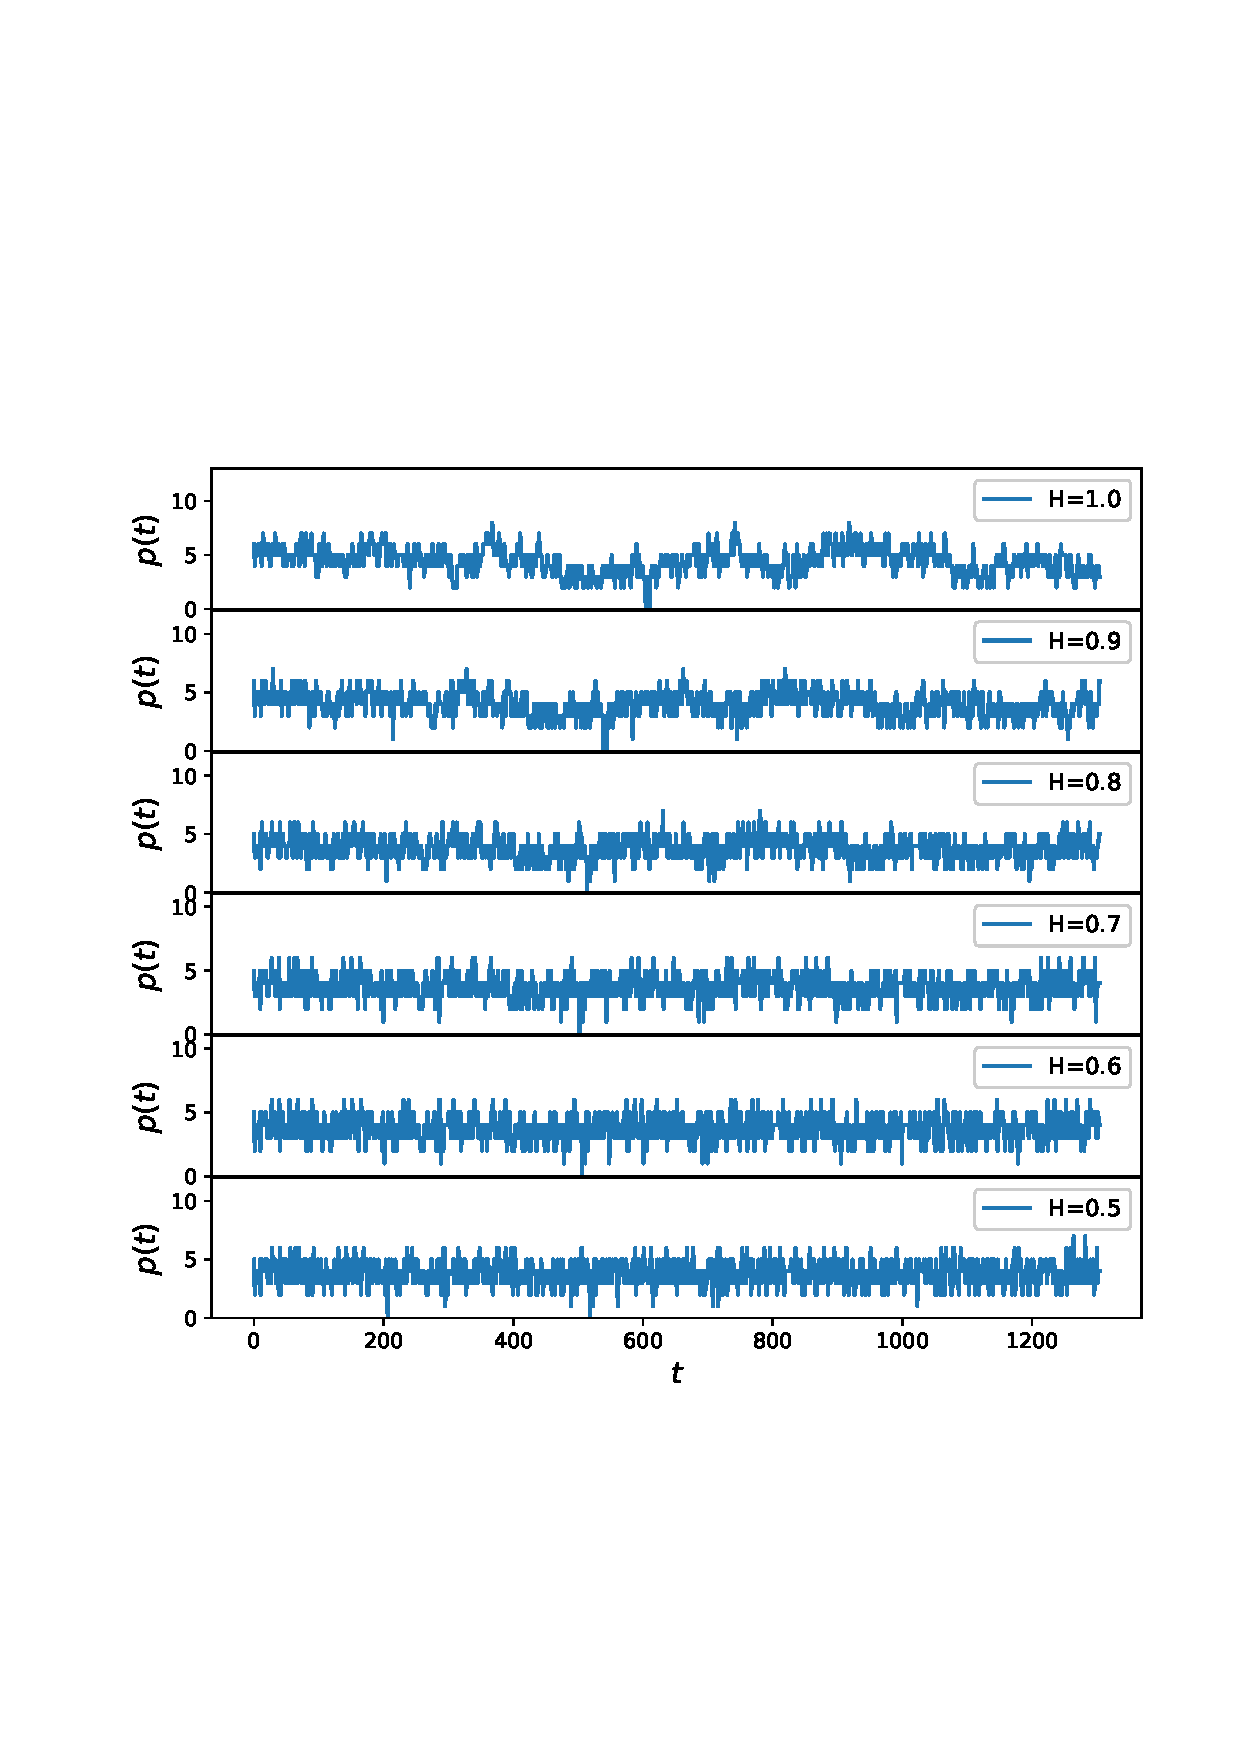
\includegraphics[width=0.7\linewidth]{Figures/monofractals.png}
	
	\caption{Monofractal signals}\label{fig:monofractals}
\end{figure}

Figure \ref{fig:monofractals} shows artificial signals generated using Fourier transform method for different values of Hurst exponents. The obtained signals are round to integers, as in real time series integer values are present. The mean values of signals are close to $4$.

For estimation of Hurst exponent from non-stationary signal can be used detrended fluctuation analasys (DFA) \cite{kantelhardt2001} \cite{peng1994}. This method removes trends and cycles from the signal, while Hurst exponent is estimated based on residual fluctuations. Signals from real world have usually  multifractal structure and can not be described with only one value of Hurst exponent \cite{kantelhardt2002}

\subsection{Multifractal analysis}

Multifractal detrended fluctuation analysis (MFDFA) \cite{kantelhardt2002, ihlen2012} to estimate multifractal Hurst exponent H(q). For given time series $\{x_i\}$ with length N, first we define global profile in the form of cumulative sum, equation \ref{eq:cumsum}, where where $\langle x\rangle $ represents average of the time series:
\begin{equation}
Y(j) = \sum_{i=0} ^j (x_i - \langle x\rangle), \quad j=1, ..., N
\label{eq:cumsum}
\end{equation}

Subtracting the mean of the time series is supposed to eliminate global trends. The profile of the signal Y is divided into $N_s = int (N/s)$ non overlapping segments of length s. If $N$ is not divisible with s the last segment will be shorter. This is handled by doing the same division from the opposite side of time series which gives us $2N_s$ segments. From each segment $\nu$, local trend $p^m_{\nu, s}$ - polynomial of order m - should be eliminated, and the variance $F^2(\nu, s)$ of detrended signal is calculated as in equation \ref{eq:var}:
\begin{equation}
F^2(\nu, s) = \frac{1}{s}\sum_{j=1}^s \left[Y(j) - p^m_{\nu, s}(j)\right]^2
\label{eq:var}
\end{equation}
Then the q-th order fluctuating function is: 
\begin{equation}
F_q(s) = \left\{\frac{1}{2N_s}\sum_{\nu}^{2N_s}\left[F^2(\nu, s)\right]^{\frac{q}{2}}\right\}^{\frac{1}{q}},  q \neq 0 \nonumber
\end{equation}
\begin{equation}
F_0(s) = \exp \left\{\frac{1}{4N_s}\sum_{\nu}^{2N_s}ln \left[F^2(\nu, s)\right]\right\}, q=0
\end{equation}

The fluctuating function scales as power-law $F_q(s) \sim s^{H(q)}$ and the analysis of log-log plots $F_q(s)$ gives us an estimate of multifractal Hurst exponent $H(q)$. Multifractal signal has different scaling properties over scales while monofractal is independent of the scale, i.e., H(q) is constant. 

\subsection{Real signals}

In this work, we use two different growth signals from real systems figure 1: (a) the
data set from TECH community from Meetup social website [36] and (b) two months
dataset of MySpace social network [37]. TECH is an event-based community where
members organize offline events through the Meetup site [36]. The time unit for TECH
is event since links are created only during offline group meetings. The growth signal
is the number of people that attend the group’s meetings for the first time. MySpace
signal shows the number of new members occurring for the first time in the dataset [37]
with a time resolution of one minute. The number of newly added nodes for the TECH
signal is N = 3217, and the length of the signal is T = 3162 steps. We have shortened
the MySpace signal to T = 20221 time steps to obtain the network with N = 10000
nodes.
\begin{figure}[!ht]
	\centering
	\includegraphics[width=\linewidth]{Figures/signals.pdf}
	\caption{Growth signals for TECH (a) and MySpace (b) social groups, their randomized counterparts, and random signal drawn from Poasonian distribution with mean $1$. The cumulative signals are shown in insets.}
	\label{fig:signals}
\end{figure}

\begin{figure}[!ht]
	\centering
	\includegraphics[width=0.6\linewidth]{Figures/hurst.pdf}
	\caption{Dependence of Hurst exponent on parameter $q$ for all five signals shown in figure \ref{fig:signals} obtained with MFDFA. }
	\label{fig:mfdfa}
\end{figure}
Real growth signals have long-range correlations, trends and cycles [37, 27, 25]. We
also generate networks using randomized signals and one computer-generated white-
noise signal to explore the influence of these signal’s features on the structure of
evolving networks. We randomize real signals using reshuffling procedure and keep their
length and mean value, the number of added nodes, and probability density function
of fluctuations intact, but destroy cycles, trends, and long-range correlations. Besides,
we generate a white-noise signal from a Poissonian probability distribution with a mean
equal to 1. The length of the signal is T = 3246, and the number of added nodes in the
final network is the same as for the TECH signal.

Figures \ref{fig:signals} (a) and \ref{fig:mfdfa} show that the TECH signal has long trends and a broad probability density function of fluctuations. The trends are erased from the randomized TECH signal, but the broad distribution of the signal and average value remain intact. MFDFA analysis shows that real signals have long-range correlations with Hurst exponent approximately $0.6$ for $q=2$, figure \ref{fig:mfdfa}. The TECH signal is multifractal, the consequence of both broad probability distribution for the values of time series and different long-range correlations of the intervals with small and large fluctuations. Shuffling of the time series does not destroy the broad distribution of values, the reason for the persistent multifractality of the TECH randomized signal, figure \ref{fig:mfdfa}.

MySpace signal has a long trend with additional cycles that are a consequence of human circadian rhythm, figure \ref{fig:signals}(b). It is multifractal for $q<0$, and has constant value of $H(q)$ for $q>0$, figure \ref{fig:mfdfa}. In MFDFA, with negative values of $q$, we put more emphasis on segments with smaller fluctuations, while for positive $q$ emphasis is more on segments with larger fluctuations \cite{ihlen2012}. Segments with smaller fluctuations have more persistent long-range correlations in both real signals, see figure \ref{fig:mfdfa}. Randomized MySpace signal and Poissonian signal are monofractal and have short-range with $H=0.5$ correlations typically for white noise.    


\section{Growing network model with aging nodes}

%The model starts with small number of nodes randomly connected. Further, at each time step new node arrives in the network and makes connection with one old node, already present in the network.
%The way in which new nodes are linked is governed by various mechanisms. They can have preference to nodes with high degree (preferential attachment), or preference to nodes with specific age. In the network model with aging nodes the probability that link is created between two nodes depends on the node degree and age \cite{hajra2004}:
%\begin{equation}
%\Pi_{i}(t)\sim k_{i}(t)^{\beta}\tau_{i}^{\alpha} 
%\label{eq:1}
%\end{equation}
%where $k_{i}(t)$ is a degree of a node $i$ at time $t$, and $\tau_{i}$ is age difference between node $i$ and newly added node. 

%The values of model parameters $\beta$ and $\alpha$ control the topology of networks.  For example if we fix $\beta=1$ and $\alpha=0$ generated networks are scale-free; degree distribution is $P(k) \sim k^{-\gamma}$ with $\gamma=3$, while in the case of nonlinear preferential attachment $\beta \neq 1$ and $\alpha=0$ scale-free properties disappear. Scale-free property can be produced along the critical line $\beta(\alpha^{*})$ in the $\alpha-\beta$ phase diagram, see Figure \ref{fig:diagram}. For $\alpha>\alpha^{*}$ networks have gel-like small world behavior, while for $\alpha<\alpha^{*}$ but close to line $\beta(\alpha^{*})$ networks have stretched exponential shape of degree distribution \cite{hajra2004}.  

%\begin{figure}[!ht]
%	\centering
%	\includegraphics[width=0.5\linewidth]{Figures/diagram.png}
%	\caption{Phase diagram of aging network model}
%	\label{fig:diagram}
%\end{figure}


The networks generated with constant growth signal are uncorrelated trees. 

To enable formation of clusters in the network new nodes need to create more than one link. We adapt the original model such that at each time step we add $M\geq1$ new nodes that make $L\geq1$ links with existing nodes in the network corresponding to probability \ref{eq:1}. 
The master equation for $N_k$, $k$ degree nodes can be written as:

\begin{equation}
\partial_{t}N_{k}=\sum^{M(t)}_{j=1}r_{k-j\longrightarrow k}N_{k-j}-\sum^{M(t)}_{j=1}r_{k\longrightarrow k+j}N_{k}+M(t)\delta_{k,L} . \label{eq:aging_master}  
\end{equation}

At each time step we add $M(t)$ nodes with $L$ links. As multiply links between two nodes are not allowed, we'll get $M(t)$ new nodes with degree $L$, that describes third term in the equation. Old nodes can increase their degree from 1 to $M(t)$, as same node can be chosen by different new nodes. The first term in the equation describes nodes with degree $k\in\{k-M(t),\ldots, k-1\}$ that getting degree $k$, while in second term nodes with degree $k$ entering degree  $k\in\{k+1,\ldots, k+M(t)\}$. The quantities $r_{k-j\longrightarrow k}$ and $r_{k\longrightarrow k+j}$ are the rates that express the transitions of a node from class with degree $k-j$ to one with degree $k$ and from class with degree $k$ to class with degree $k+j$ respectively. 

The equation \ref{eq:aging_master} is not solvable in a general case. It was solved for the case $M(t)=1$ and specific values of parameters $\alpha$ and $\beta$ using continuous approach \cite{dorogovtsev2001b}. In this work, we use numerical simulations to explore the case when $M(t)$ is a correlated time-varying function and study how these properties influence the structure of generated networks for different values of parameter $-\infty<\alpha\leq-1$ and $\beta\geq1$ and constant $L$.


\section{Structural differences between networks }

%\subsection{D-measure}

%Between two nodes in the network, we can define different paths, but the most important one are the shortest paths, $d_{ij}$. Diameter defines the largest shortest path found in the network. For each node $i$ we can define the distribution of the shortest paths between node $i$ and all others nodes in the network, $P_{i}=\{p_{i}(j)\}$, where $p_{i}(j)$ is percent of nodes at distance $j$ from node $i$. The connectivity patterns can efficiently describe difference between two networks.    
%To specify how much $G$ and $G^{'}$ are similar we use D-measure \cite{tiago2}

%\begin{equation} 
%\label{eq:dmeasure}
%D(G,G') = \omega \left| \sqrt{\frac{J(P_1,..P_N)}{log(d)}}-\sqrt{\frac{J(P_1^{'},..P_N^{'})}{log(d^{'})}} \right| \nonumber +  (1-\omega) \sqrt{\frac{J(\mu_{G},\mu_{G^{'}})}{log2}}.
%\end{equation}

%D-measure calculates Jensen-Shannon divergence between $N$ shortest path distributions, $J(P_1,.., P_N)) = \sum_{i,j}p_i(j)log(\frac{p_i(j)}{\mu_j})$, where  $\mu_j = (\sum_{i=1}^N p_i(j))/N$ is mean shortest path distribution. The first term in equation \ref{eq:dmeasure} compares local differences between two networks, and Jensen-Shannon divergence between $N$ shortest path distributions $J(P_{1},...,P_{N})$ is normed with network diameter $d$. The second part determines global differences, computing  ${J(\mu_{G},\mu_{G^{'}})}$ between mean shortest path distributions. We consider equally important local and global properties of the networks, and parameter $\omega$ is set to $0.5$. The D-measure ranges from $0$ to $1$. The lower D-measure is, networks are more similar and for D-measure $D = 0$, structures are isomorphic.

The advantage this measure has is that it can distinguish between networks generated with the same model parameters. To examine how different growth signals influence the network structure, we use D-measure and compare networks generated with the same model parameters $\alpha$, $\beta$ and fixed number of links per new node $L$, but different growth signals. The growth of first network is driven by fluctuating signal $M_1 = {M(t)}$, while the other one grows by constant rate $M_2=<M(t)> = const$. 

We focus on the region of model phase diagram with negative $\alpha$ and positive $\beta$ as there is found the transition line from stretched-exponential across scale-free to the small world- gel networks. We take range of parameters  $-3\leq\alpha\leq-0.5$ and $1\leq\beta\leq3$ with steps $0.5$ and we also vary the the number of links each new node can create $L\in{1, 2, 3}$. For each combination of $(\alpha, \beta, L)$ we generate the sample of $100$ networks, and compare the structure of network grown with fluctuating and the constant signal. The results represented by D-measure are obtained averaging the D-measure between all possible pairs of generated networks.     

\begin{figure}[h!]
	\centering
	\includegraphics[width=0.5\textwidth]{Figures/Ddist_M4_w10.5_w20.5.png}
	\caption{D-distance between networks generated with different long-range correlated signals with fixed value of Hurst exponent and networks generated with constant signal M=4.}
	\label{fig:Ddist_m}
\end{figure}

First, we explore how monofractal signals, see Figure \ref{fig:monofractals} shape the structure of complex networks. The D-measure between networks grown with monofractal signal, with $H \in \{0.5, 0.6, 0.7, 0.8, 0.9, 1.0\}$ and constant signal $M=4$ are shown in figure \ref{fig:Ddist_m}. The higher values of D-measure are found in the region of critical line $\beta(\alpha^{*})$. The most considerable influence is on networks with scale-free distribution. Comparing D-distance in only one point of  phase diagram, for example $L=1, \alpha = -2.5, \beta = 2.5$, we find correlations in the signal (Hurst exponent is larger), make bigger impact on the network structure. D-measure between networks grown with signal with Hurst exponent $H=1.0$ and constant signal is $D(H=1.0, M=4) = 0.405$, while between networks grown with signal with $H=0.8$ and constant signal is $D(H=0.8, M=4) = 0.316$. For $\alpha>\alpha^{*}$ networks have similar structural properties and D-measure is close to 0. In the region of networks with stretched exponential degree distribution $\alpha<\alpha^{*}$  differences are small.  

For signals from real communities we find non-zero values of D-measure \ref{fig:dmeasure}. The largest difference between networks is as before along critical line $\beta(\alpha^{*})$, for scale free network. For values $\beta<\beta(\alpha^{*})$ the structural differences exist, but they become smaller. In the region of gel small world networks $\alpha>\alpha^{*}$ structural differences are small and close to zero. In the region around critical line we find that D-measure depends on the properties of the signal. Multifractal signals TECH has the largest impact on network structure; the maximum obtained value of D-measure is $D_{max}=0.552$. Similar behavior we discover for other multifractal signals, random TECH and MySpace. For networks generated with uncorelated signals, random mySpace and Poisson, difference exists but it is much smaller and comparable with monofractal signals.  


\begin{figure}[h!]
	\centering
	\includegraphics[width=0.5\linewidth]{Figures/Ddistance.pdf}
	\caption{The comparison of networks grown with growth signals shown in figure \ref{fig:signals} versus ones grown with constant signal $M=1$, for value of parameter $\alpha\in[-3,-1]$ and $\beta\in[1,3]$. $M(t)$ is the number of new nodes, and $L$ is the number of links added to the network in each time step. The compared networks are of the same size.}
	\label{fig:dmeasure}
\end{figure}

The position of the critical line slightly moves toward larger $\beta$ with higher link density $L$. The addition of more than one node does not influence its position. Although, for fixed network density, we find a critical line independent of the growth signal's properties as can be seen in Figures \ref{fig:dmeasure}, \ref{fig:Ddist_m}. 

We can note that D-measure rises for lower $\alpha$. In the case of constant signal, number of nodes added to the network is equal for each time step, so at time interval $T$ the network has $MT$ nodes. In fluctuating signal the number of nodes  added during time interval $T$ vary with time. In signals, such as TECH, where are present peaks in the number of new users, emergence of hubs happens faster. As we decrease the parameter $\alpha$, fluctuations present in the signal become more important and emergence of the hubs happens even for uncorrelated signals. The trends present in the real signals further promote the emergence of hubs in the network.    

\subsection{The assortativity and clustering}

We further explore the assortativity index and clustering coefficient of networks generated with monofractal signals with different values of Hurst exponent. We show results for several ageing model parameters to show the difference between network this model can produce, \ref{fig:aindex}. All networks are disassortative, with a negative degree-degree correlation index. For the values of parameters below critical line, $\alpha=-2.5, \beta=1.5$ $r$ does not depend on the Hurst exponent. Above the critical line are small-world networks, and they are disassortative with a minimum value of assortativity index $r =-1$, for $L=1$, indicating the presence of a hub that connects to many nodes. The assortativity index slightly grows with link density. 

In the region of critical parameters, the assortativity index depends on the value of the Hurst exponent. The larger influence on the assortativity index have correlated signals, with Hurst exponent $H>0.8$, so networks become more disassortative, see line for parameters $L=1, \alpha=-2.5, \beta=2.5$ in Figure \ref{fig:aindex}. The long-range correlations have a stronger effect on the evolution of networks with lower density. 

We calculate the mean clustering coefficient, Figure \ref{fig:aindex}. For $L=1$ networks are uncorrelated trees, with clustering coefficient $0$. For network density $L>1$, nodes are organized into clusters. Under the critical line, for parameter  $L=3, \alpha=-2.5, \beta=1.5 $, clustering coefficient is constant and low. Similar values are obtained for clustering coefficient for critical parameters $L=3, \alpha=-1.5, \beta=2.0$, but for Hurst exponent $H>0.8$ clustering coefficient increase. Small world networks,  $L=3, \alpha=-1.5, \beta=2.5$ are clustered, the value of $<c>$ is high.  The value of clustering for networks created with the constant signal is 0.8. Networks grown with white noise signal and signal with H=0.6 have higher values of the clustering, while networks grown with signals that have Hurst exponent larger than 0.6 have the same value of clustering, which is below 0.8. 
 
\begin{figure}[h!]
	\centering
	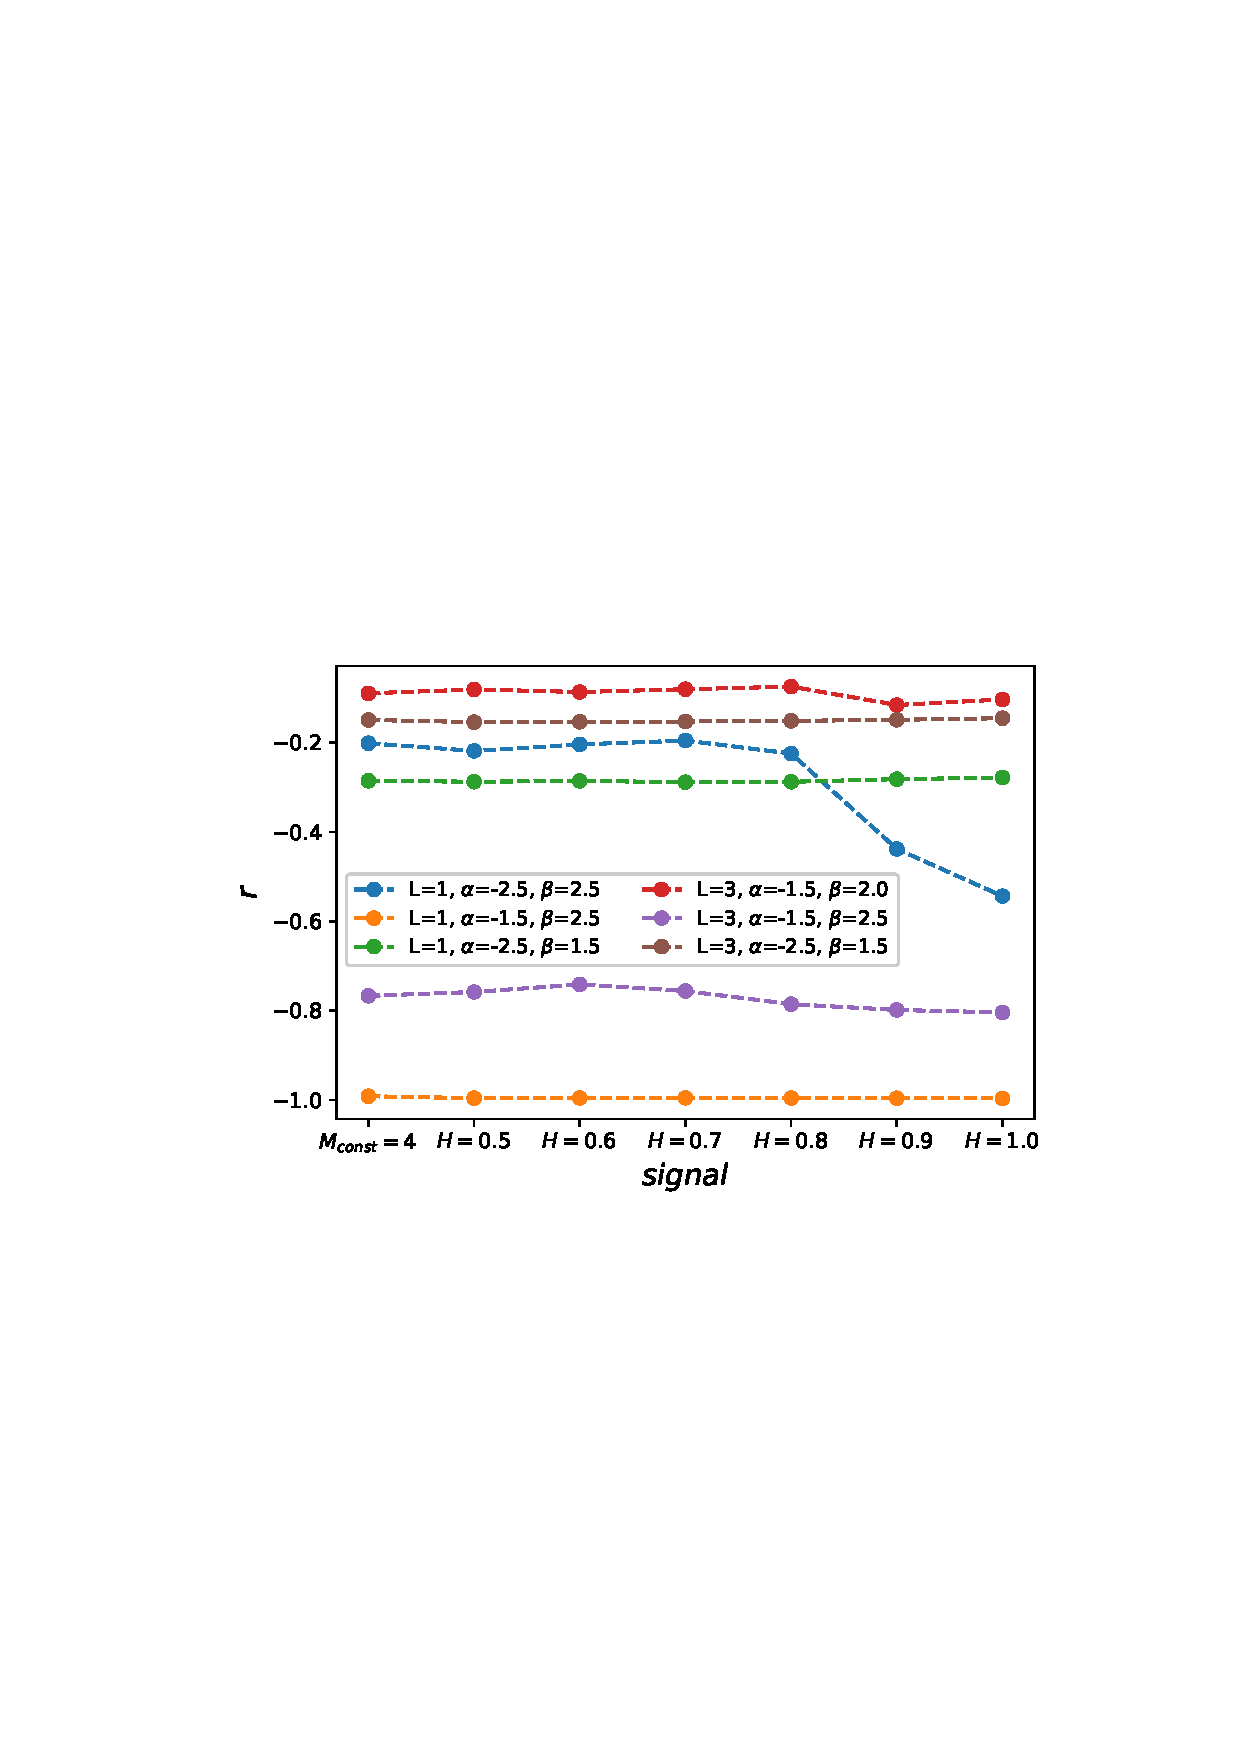
\includegraphics[width=0.45\textwidth]{Figures/aindex.png}
	\includegraphics[width=0.45\textwidth]{Figures/clustering.png}
	\caption{Aindex}
	\label{fig:aindex}
\end{figure} 

We examine degree distribution, degree correlations and clustering coefficient of networks generated by real signals, as researchers has shown that these measures provide the sufficient set for discribing structure of complex network. D-measure showed that multifractals have larger influence on networks than monofractals, especially on scale-free networks. 

Figure \ref{fig:properties_sf} shows properties of networks generated with model parameters $L=2$, $\alpha=-1.0$, $\beta=1.5$, that lies on critical line.  The degree distributions $P(k)$ of networks generated with real signals TECH and MySpace have emergence of super-hubs. Degree distributions generated with randomized signals and white noise signal do not differ from degree distribution of networks generated with constant signal. Networks generated with real signals average neighbouring degree $\langle k\rangle_{nn}(k)$ and clustering coefficient $c(k)$ depend on node degree, while in networks generated with constant and randomized signals they weakly depend on the degree $k$.

\begin{figure}[h!]
	\centering
	\includegraphics[width=0.7\textwidth]{Figures/b1.pdf}
	\caption{Degree distribution, the dependence of average first neighbor degree on node degree, dependence of node clustering on node degree for networks grown with different time-varying and constant signals. Model parameters have value $\alpha=-1.0$, $\beta=1.5$  and $L=2$ for all networks. The networks are from scale-free class.}
	\label{fig:properties_sf}
\end{figure}

We also find structural differences between networks, obtained with model parameters under the critical line $\alpha<\alpha^{*}$, see Figure \ref{fig:properties_se}. The difference is mostly found for TECH signal. Degree distribution $P(k)$ shows emergence of hubs in networks grown with TECH signal, while the randomized and Poisson signal are more similar to networks grown with constant signal. MySpace signal; whose generalized Hurst exponent $H(q)$ weakly depends on scale parameter $q$ and whose long-range correlations and trends are easily destroyed; do not influence the structure of networks more than constant or randomized signal.   

\begin{figure}[h!]
	\centering
	\includegraphics[width=0.7\textwidth]{Figures/b3.pdf}
	\caption{Degree distribution, the dependence of average first neighbor degree on node degree, dependence of node clustering on node degree for networks grown with different time-varying and constant signals. Model parameters have value $L=2, \alpha=-1.5$, $\beta=1.5$. The networks have stretched exponential degree distribution.}
	\label{fig:properties_se}
\end{figure}

The properties of time-varying signal do not influence the topological properties of small-world gel networks, Figure \ref{fig:properties_sw}. Here model promote existence of hubs. As this is mechanism through which the fluctuations alter the structure of evolving networks, the properties of the signal are not relevant.  


\begin{figure}[h!]
	\centering
	\includegraphics[width=0.7\textwidth]{Figures/b2.pdf}
	\caption{Degree distribution, the dependence of average first neighbor degree on node degree, dependence of node clustering on node degree for networks grown with different time-varying and constant signals. Model parameters have value $ L=2, \alpha=-1.0$, $\beta=2.0$. Generated networks have scale-free properties.}
	\label{fig:properties_sw}
\end{figure}


\newpage 
\section{Conclusions}

We demonstrate that the resulting networks' structure depends on the features of the time-varying signal that drives their growth. The previous research \cite{mitrovic2012,mitrovic2015} indicated the possible influence of temporal fluctuations on network properties. Our results show that the temporal properties of growth signals generate networks with power-law degree distribution, non-trivial degree-degree correlations, and clustering coefficient even though the local linking rules, combined with constant growth, produce uncorrelated networks for the same values of model parameters \cite{hajra2004}. 

We observe the most substantial dissimilarity in network structure along the critical line, the values of model parameters for which we generate networks with broad degree distribution. Figure \ref{fig:dmeasure} shows that dissimilarity between networks grown with time-varying signals and ones grown with constant signals always exists along this line regardless of the features of growth signal. However, the magnitude of this dissimilarity strongly depends on these features. We observe the largest structural difference between networks grown with multifractal TECH signal and networks that evolve by adding one node in each time step. The identified value of D-measure is similar to one calculated in the comparison between sub-critical and super-critical Erd\"{o}s–R\'{e}nyi graphs \cite{tiago2} indicating the considerable structural difference between these networks. Our findings are further confirmed in figure \ref{fig:properties}(b). The networks generated with signals that have trends and long-range temporal correlations differ the most from those grown with the constant signal. Our results show that even white-noise type signals can generate networks significantly different from ones created with constant signal for low values of $\alpha^{*}$.

The value of D-measure declines fast as we move away from the critical line, figure \ref{fig:dmeasure}. The main mechanism through which the fluctuations influence the structure of evolved networks is the emergence of hubs and super hubs. For values of $\alpha<<\alpha^{*}$, the nodes attache to their immediate predecessors creating regular networks without hubs. For $\alpha \sim \alpha^{*}$ graphs have stretched exponential degree distribution with low potential for the emergence of hubs. Still, multifractal signal TECH enables the emergence of hub even for the values of parameters for which we observe networks with stretched-exponential degree distribution in the case of constant growth figure \ref{fig:properties}(a). By definition, small-world gels generated for $\alpha>\alpha^{*}$ have super-hubs \cite{hajra2004} regardless of the growth signal, and therefore the effects that fluctuations produce in the growth of networks do not come to the fore for values of model parameters in this region of $\alpha-\beta$ plane.

Evolving network models are an essential tool for understanding the evolution of social, biological, and technological networks and mechanisms that drive it \cite{boccaletti2006}. The most common assumption is that these networks evolve by adding a fixed number of nodes in each time step \cite{boccaletti2006}. So far, the focus on developing growing network models was on linking rules and how different rules lead to networks of various structural properties \cite{boccaletti2006}. Growth signals of real systems are not constant \cite{mitrovic2015,mitrovic2012}. They are multifractal, characterised with long-range correlations \cite{mitrovic2015}, trends and cycles \cite{suvakov2013}. Research on temporal networks has shown that temporal properties of edge activation in networks and their properties can affect the dynamics of the complex system \cite{holme2012}. Our results imply that modeling of social and technological networks should also include non-constant growth and that its combination with local linking rules can significantly alter the structure of generated networks.

%----------------------------------------------------------------------------------------



%% Chapter 1

\chapter{Groups growth model} % Main chapter title


Social groups, informal or formal, are mesoscopic building elements of every socio-economic system that direct its emergence, evolution, and disappearance \cite{}. The examples span from countries, economies and science to society in general. Settlements, villages, towns and cities are formal and highly structured social groups of countries. Their organisation and growth determine the functioning and sustainability of every society \cite{barthelemy2016structure}. Companies are the building blocks of an economic system and their dynamics are important indicators of the level of its development \cite{hidalgo2009building}. Scientific conferences, as scientific groups, enable fast dissemination of the latest results, exchange and evaluation of ideas as well as a knowledge extension, and thus are an integral part of science \cite{smiljanic2016theoretical}. The membership of individuals in various social groups, online and offline, can be essential when it comes to the quality of their life \cite{montazeri2001anxiety, davison2000talks, cho2012tea}. Therefore, it is not surprising that the social group emergence and evolution are at the center of the attention of many researchers \cite{aral2012identifying,gonzalez2013broadcasters, torok2013opinions, yasseri2012dynamics}.

%Thanks to big data availability, we have more information to understand the behavior of social systems. 
Along with massive data sets comes the need to develop methods and tools for their analysis and modeling. Methods and paradigms from statistical physics have proven to be very useful in studying the structure and dynamics of social systems \cite{castellano2009statistical}. The main argument for using statistical physics to study social systems is that they consist of many interacting individuals. Due to this, they exhibit different patterns in their structure and dynamics, commonly known as \textit{collective behavior}. While building units of a social systems can be characterized by many different properties, only few of them enforce collective behavior in the systems. The phenomenon is known as \textit{universality} in physics and is commonly observed in social systems such as in voting behavior \cite{chatterjee2013universality}, or scientific citations \cite{radicchi2008universality}. It indicates the existence of the universal mechanisms that govern the dynamics of the system \cite{}.


The availability of large-scale and long-term data on various online social groups has enabled the detailed empirical study of their dynamics. The focus was mainly on the individual groups and how structural features of social interaction influence whether individuals will join the group \cite{backstrom2006group} and remain its active members \cite{smiljanic2016theoretical, smiljanic2017associative}. The study on LiveJournal \cite{backstrom2006group} groups has shown that decision of an individual to join a social group is greatly influenced by the number of her friends in the group and the structure of their interactions. The conference attendance of scientists is mainly influenced by their connections with other scientists and their sense of belonging \cite{smiljanic2016theoretical}. The sense of belonging of an individual in social groups is achieved through two main mechanisms \cite{smiljanic2017associative}: expanding of the social circle at the beginning of joining the group and strengthening of the existing connections in the later phase. The dynamics of social groups depend on their size \cite{}. Analysis of the evolution of large-scale social networks has shown that edge locality plays a critical role in the evolution of social networks \cite{leskovec2008microscopic}. Small groups are more cohesive with continued membership, while large groups tend to change their active members constantly \cite{PNAS}. These findings help us understand the growth of a single group, the evolution of its social network, and the influence of the network structure on the group growth. However, how the growth mechanisms influence the distribution of members of one social system among groups is still anecdotal.

Furthermore, it is not clear whether the growth mechanisms of social groups are universal or system-specific. The size distribution of social groups has not been extensively studied. Rare empirical evidence of the size distribution of social groups indicates that it follows power-law behavior \cite{zheleva2009co}. However, the distribution of company sizes follows log-normal behavior and remains stable over decades \cite{amaral1997scaling, stanley1996scaling}. Analysis of the sizes of the cities shows that the distribution of all cities also follows a log-normal distribution. In contrast, the distribution of the largest cities resembles Zipf's distribution \cite{fazio2015pareto}.

A related question that should be addressed is whether we can create a unique yet relatively simple microscopic model that reproduces the distribution of members between groups and explains the differences observed between social systems. French economist Gibrat proposed a simple growth model to reproduce the observed log-normal size distribution of companies and cities. However, the analysis of the growth rate of the companies \cite{amaral1997scaling} has shown that growth mechanisms are different from ones assumed by Gibrat. In addition, the analysis of the growth of three online social networks showed that population growth is not determined by the population size and spatial factors, and it deviates from Gibrat's law \cite{zhu2014online}. Other mechanisms, for instance, growth through diffusion, have been used for modeling and prediction of rapid group growth \cite{kairam2012life}. However, the growth mechanisms of various social groups and the source of the scaling observed in socio-economic systems remain hidden.

Here we analyze the size distribution of formal social groups in two different systems: Meetup online platform and subreddits on Reddit. We are interested in the scaling behavior of size distributions and the distribution of growth rates. Empirical analysis of the dependence of growth rates, shown in this work, indicates that growth cannot be explained through Gibrat's model. Here we contribute with a simple microscopic model that incorporates some of the findings of previous research \cite{backstrom2006group, zheleva2009co}. We show that the model can reproduce size distributions and growth rate distributions for both studied systems. Moreover, the model is flexible and can produce a broad set of size distributions depending on the value of model parameters.

The paper is organized as follows: in Section \ref{sec:data} we describe the data, while in Section \ref{sec:emp} we present our empirical results. In Section \ref{sec:model} we introduce model parameter and rules. In section \ref{sec:results} we demonstrate that model can reproduce the growth of social groups in both systems and show the results for different values of model parameters. Finally, in Section \ref{sec:con}, we present concluding remarks and discuss our results. 

\section{Data \label{sec:data}}
We analyse the growth of social groups from two widely used online platforms: Reddit and Meetup. Reddit \footnote{https://www.reddit.com/} enables sharing diverse web content and members of this platform interact exclusively online through posts and comments. The Meetup \footnote{www.meetup.com} allows people to use online tools to organize offline meetings. The building elements of the Meetup system are topic-focused groups, such as food lovers or ICT and data science professionals. Due to their specific activity patterns - events where members meet face-to-face - Meetup groups are geographically localised. 

%Reddit \footnote{https://www.reddit.com/} enables sharing diverse web content, while Meetup \footnote{www.meetup.com} allows people to use online tools to organize offline meetings. Reddit s interact exclusively online through posts and comments. The building elements of the Meetup system are topic-focused groups, such as food lovers or ICT and data science professionals. Due to their specific activity patterns - events where members meet face-to-face - Meetup groups are geographically localised. 


We compiled the Reddit data from https://pushshift.io/. This site collects data daily and, for each month, publishes merged comments and submissions in the form of JSON files. 
Specifically, we focus on subreddits - social groups of Reddit members interested in a specific topic. 
We select subreddits active in 2017 and follow their growth from their beginning until $2011-12$. The considered dataset contains 17073 subreddits with $2 195 677$ active members, with the oldest originating from 2006 and the youngest being from 2011. For each post under a subreddit, we extracted the information about the member-id of the post owner, subreddit-id, and timestamp. As we are interested in the subreddits growth in the number of members, for each subreddit and member-id we selected timestamp when member made a post for the first time. Finally, in the dataset we include only subreddits active at least two months.  

%We compiled the Reddit data from https://pushshift.io/. This site collects data daily and, for each month, publishes merged comments and submissions in the form of JSON files. Specifically, we focus on subreddits - social groups of Reddit members interested in a specific topic. 
%We select all subreddits active in 2017 and follow their growth from their beginning until 2011. The considered dataset contains 17000 subreddits, with the oldest originating from 2006 and the youngest being from 2011.\\
%%We select all subreddits active in 2012 and follow their growth from their beginning until 2017. The considered dataset contains 17000 subreddits, with the oldest originating from 2003 and the youngest being from 2017.\\
%For each post under a subreddit, we extracted the information about the user-id of the post owner, subreddit-id, and timestamp. We observed the data from $2006$ to the $2017$ year, and for each subreddit and user-id, we selected timestamp when a user made a post for the first time. For our analysis, we chose subreddits still active in $2017$ while removing small subreddits active for less than a month. The resulting dataset contains $304 007$ subreddits and  $36 595 134$ users.

%For simulation, we extracted data until $2011-12$ and removed all subreddits, active less than one month. 
%with a small amount of activity.
%This reduced the dataset significantly - we obtained only $17 073$ subreddits with $2 195 677$ active users. \\

The Meetup data were downloaded in $2018$ using public API. The Meetup platform was launched in 2003, and at the moment we accessed the data, there were more than 240 000 active groups. For each group, we extracted information about the date it had been founded, its location, and the total number of members. We focused on the groups founded from $2003$ until $2017$ in big cities London and New York, where Meetup platform achieved considerable popularity. We considered groups active at least two months. There were 4673 groups with 831685 members in London and 4752 groups with 1059632 members in New York. In addition, we extracted the id of each member in the group and the information about organised events. This allowed us to obtain the date when a member joined a group, which is the first time she attended group event. 

In both systems, we approximated the timestamp when the member joined the group. Based on this information, we can calculate the number of new members per month $N_{i}(t)$, the group size $S_{i}(t)$ at each time step, and the growth rate for the group in both systems. The time step for both systems is one month. The size of the group $i$ at time step $t$ is the number of members that joined that group ending with the month, i.e., $S_{i}(t)=\sum^{k=t}_{k=t_{i0}}N_{i}(t)$, where $t_{i0}$ is the time step in which the group $i$ was created. We do not consider when a member leaves a group or subreddit since this kind of information is not available to us. For these reasons, the size of considered groups is a non-decreasing function. The growth rate $R_i(t)$ at step $i$ is obtained as logarithm of successive sizes $R = log(S_{i}(t)/S_{i}(t-1))$. 

While the forms of communication between members and activities that members engage in differ in those two systems, some common properties exist between them. Members can form a new groups and join existing ones in both systems. Furthermore, each member can belong to an unlimited number of groups. For these reasons, we can use the same methods to study and compare the formation of groups in Reddit and Meetup. 


%From collected data, for each group, we calculate the number of new members per month $N_{i}(t)$, the group size $S_{i}(t)$ at each time step, and the growth rate for group in both systems. Time step for both systems is one month. The size of the group $i$ at time step $t$ is the number of members that joined that group ending with the month, i.e., $S_{i}(t)=\sum^{k=t}_{k=t_{i0}}N_{i}(t)$, where $t_{i0}$ is the time step in which the group $i$ was created. The growth rate $R_i(t)$ at step $i$ is obtained as logarithm of successive sizes $R = log(S_{i}(t)/S_{i}(t-1))$. 

%While these two systems differ in means of communication between their members and activities their members engage in, there are certain common properties that enable us to use same methods to study the growth of groups in these systems and make a comparative analysis of this growth. In both systems, members can create new groups and join existing ones. One member can belong to unlimited number of groups/subreddits at the same time. The number of groups in the systems is also unlimited. For each meetup group we have an information on when member has attended first group event. Based on this information we can infere the size of each group for each month. For a subreddit we have a detailed information about members' activity and thus we have an information when a user made a first post in specific subreddit. This moment is considered as the moment when the member has joined the subreddit and became an active member. In our case we do not take into account when a member leaves a group or subreddit, since this kind of information is not available to us. For these reasons, the size of considered groups is non-decreasing function. 

\section{Empirical analysis of social group growth \label{sec:emp}}
\begin{figure}[h!]
	\centering
	\includegraphics[width=0.8\linewidth]{Figures/figures/Fig2.png}
	\caption{The number of groups over time, normalized sizes distribution, normalized log-rates distribution and dependence of log-rates and group sizes for Meetup groups created in London from 08-2002 until 07-2017 that were active in 2017 and subreddits created in the period from 01-2006 to the  12-2011 that were active in 2017. }
	\label{fig:data1}
\end{figure}

Figure \ref{fig:data1} summarize properties of the groups in Meetup and Reddit systems. The number of groups grows exponentially over time. Nevertheless, we notice that Reddit has substantially larger number of groups than Meetup. The Reddit groups are prone to engage more members in a shorter period of time. Size of the Meetup groups is in the range from several members up to several tens of thousands of members, while sizes of subreddits are between a few tens of members up to several millions.
The distributions of group sizes follows the lognormal distribution
\begin{equation}
P(S)=\frac{1}{S\sigma\sqrt{2\pi}}exp(-\frac{(\ln(S)-\mu)^{2}}{2\sigma^{2}})
\label{eq:log} \ ,
\end{equation}
where $S$ is the group size and $\mu$ and $\sigma$ are parameters of the distribution. We used package \cite{powerlaw} to fit Eq. \ref{eq:log} to Reddit and Meetup data and found that distribution of groups sizes for Meetup groups in London and New York follow similar distributions with the values of parameters $\mu= -0.93$, $\sigma = 1.38$ and $\mu=-0.99$ and $\sigma=1.49$ for London and New York respectively. The distribution of sizes of subreddits also has the log-normal shape with parameters $\mu= -5.41$ and $\sigma = 3.07$. Even though these distributions are from the same class, for subreddits we find broader distribution that may resemble power-law distribution. Our analysis shown in Supportive Information (SI) confirms that the distribution exhibits a log-normal behavior, see SI-Table 1 and SI-Fig. 1.  



The log-normal distributions can be generated by multiplicative processes \cite{mitzenmacher2004brief}. If there is a quantity with size $S_i(t)$ at time step $t$, it will grow so after time period $\delta$ the size of the quantity is $S(t+\Delta t) = S(t) r$, where $r$ represents a random process. The Gibrat law states that growth rates $r$ are uncorrelated and do not depend on the current size. In order to describe the growth of social groups, we calculate the logarithmic growth rates defined as $R = log\frac{S_t}{S_{t-\Delta t}}$. According to Gibrat law, the distribution of sizes follow log-normal distribution. For logarithmic growth rates expected distribution is normal, or as it is shown in many studies it is better explained with Laplacian (“tent  shaped“) distribution \cite{mondani2014fat}, \cite{fu2005growth}. In figure \ref{fig:data1} we calculate distributions of log-rates. For both systems, log-rates are very well approximated with log-normal distribution. The Fig. \ref{fig:data1} shows that log-rates depend on the groups size, especially for the smaller and medium size groups. Our empirical analysis implies that the growth of Meetup and Reddit groups violates the basic assumptions of the Gibrat's law \cite{frasco2014spatially, qian2014origin}, and thus, this growth can not be explained as a simple multiplicative process.\\

We are considering a relatively large time period for online groups. The fast expansion of Information Communications Technology (ICT) led to change of how members access online systems. With the use of smartphones the online systems became more available, which led to exponential growth of ICTs systems, figure \ref{fig:data1} and potential change in the mechanisms that influence growth of social groups in them. For these reasons we aggregate groups according to year they were founded for each of the three data sets and look at the distributions of these sizes in the year 2017 for Meetup groups and 2011 for Reddit. For each year and each of the three data sets we calculate the average size of the groups that were created in a year $y$ $<S^{y}>$. We normalize the size of the groups created in year $y$ with corresponding average size $s^{y}_{i}=S^{y}_{i}/<S^{y}>$ and calculate the distribution of the normalized sizes for each year. The distribution of normalized sizes for all years and all data sets is shown in figure \ref{fig:scale}. All distributions exhibit log-normal behavior. Furthermore, the distributions for the same data set and different years follow a universal curve with same value of parameters $\mu$ and $\sigma$. The universal behavior is observed for distribution of normalized log-rates as well, see Fig. \ref{fig:scale} (bottom panel). These results indicate that growth of the social groups did not change due to increased growth of members in systems. Furthermore, it implies that the growth is independent of the size of the whole data set.   

\begin{figure}[!h]
	\centering
	\includegraphics[width=0.8\linewidth]{Figures/figures/Fig1.png}
	\caption{The figure shows the groups' sizes distributions and log-rates distributions. Each distribution collects groups founded in the same year and is normalized with its mean value. The group sizes are at the end of 2017 for meetups and 2011 for subreddits. }
	\label{fig:scale}
\end{figure}

%\newpage

%\subsection{Meetup data processing}

%\subsection{Reddit data processing}



%\\
%(1) We use reddit database publicly available from https://pushshift.io/ \\
%(2) The database includes submissions and comments posted on different subreddits. For each post, we have information about who posted it (user-id), when (timestamp) and on what subreddit (subreddit-id). \\
%(3) First, for each subreddit, in each month, we filtered number of users who posted for the first time in the community. Excluding subreddits with activity less than month, we end up with 483872 different subreddits. \\
%(4) Next we filtered subreddits that had activity in 2017 (by activity we mean, newcomers activity)\\
%(5) For simulations we selected data until 2012.

\section{Model \label{sec:model}}
Growth of social groups can not be explained with the simple rules of Gibrat's law. Previous research on group growth and longevity has shown that social connections with members of a group influence individual's choice to join that group \cite{kairam2012life, zheleva2009co}. Moreover, individual's interests and the need to discover new content or activity also influence diffusion of individuals between groups. Furthermore, social systems constantly grow since new members join every minute. The properties of the growth signal that describes the arrival of new members influence both dynamics of the system \cite{mitrovic2011quantitative, dankulov2015dynamics} and the structure of social interactions \cite{vranic2021growth}. Furthermore, number of social groups in the social systems is not constant. They are constantly created and destroyed.

In Ref. \cite{zheleva2009co} authors propose the co-evolution model of the growth of social networks. In this model, authors assume that social system evolves trough co-evolution of two networks: network of social contacts between members and network of members' affiliations with groups. This model addresses the problem of growth of social networks that includes both linking between members and social group formation. In this model, a member of a social system selects to join a group either through random selection or according to her social contacts. In the case of random selection, there is a selection preference toward larger groups. If member chooses to select a group according to her social contacts, the group is selected randomly from the list of groups with which her friends are already affiliated.

While the co-evolution model \cite{zheleva2009co} was not created with the intent of studying the growth and size distribution of social groups, authors show that their model is able to reproduce distribution of group sizes for several online social networks that follow power-law distribution. Our empirical analysis, shown in Sec. \ref{sec:emp} shows that distribution of group sizes is not always power-law, indicating that certain mechanisms proposed in co-evolution model are not universal for all social systems. To fill the gap in understanding how social groups in social system grow, we propose a model of group growth that combines random and social diffusion between groups but following different rules than co-evolution model \cite{zheleva2009co}.\\

\begin{figure}[h!]
	%%% OVO JE MOZDA PREVISE PA AKO MISLITE MOZEMO I DA IZBACIMO ili ostavimo samo ovaj donji panel.
	\centering
	\includegraphics[scale=0.5]{Figures/figures/test.png}
	\caption{The top panel shows bipartite (member-group) and social (member-member) network. Filled nodes are active members, while thick lines are new links in this time step. In the social network dashed lines show that members are friends but still do not share same groups. The lower panel shows model schema. \textbf{Example:} member $u_6$ is a new member. First it will make random link  with node $u_4$, and then with probability $p_g$ makes new group $g_5$. With probability $p_a$ member $u_3$ is active, while others stay inactive for this time step. Member $u_3$ will with probability $1-p_g$ choose to join one of old groups and with probability $p_{aff}$ linking is chosen to be social. As its friend $u_2$ is member of group $g_1$, member $u_3$ will also join group $g_1$. Joining group $g_1$, member $u_3$ will make more social connections, in this case it is member $u_1$.}
	\label{fig:schema}
\end{figure}

Figure \ref{fig:schema} shows a schematic representation of our model. Similar to co-evolution model \cite{zheleva2009co}, we represent social system with two evolving networks, see Fig. \ref{fig:schema}. One network is bipartite network which describes the affiliation of individuals to social groups $\mathcal{B}(V_{U}, V_{G}, E_{UG})$. This network consists of two partitions, members $V_{U}$ and groups $V_{G}$, and set of links $E_{UG}$, where a link $e(u,g)$ between a member $u$ and a group $g$ represents the member's affiliation with that group. Bipartite network grows through three activities: arrival of new members, creation of new groups, and through members joining groups. By definition, in bipartite networks links only exist between nodes belonging to different partitions. However, as we explained above, social connections affect whether a member will join a certain group or not. In the simplest case, we could assume that all members belonging to a group are connected with each other. However, previous research on this subject \cite{ smiljanic2017associative, backstrom2006group, zheleva2009co} has shown that the existing social connections of members in a social group are only a subset of all possible connections. For these reasons, we introduce another network $\mathcal{G}(V_{U},E_{UU})$ that describes social connections between members. The social network grows through addition of new members to the set $V_{U}$ and creation of new links between them. The member partition in bipartite network $\mathcal{B}(V_{U}, V_{G}, E_{UG})$ and set of nodes in members' network $\mathcal{G}(V_{U}, E_{UU})$ are identical.\\

For convenience, we represent bipartite and member networks with adjacency matrices $B$ and $A$. The element of matrix $B_{ug}$ equals one if member $u$ is affiliated with group $g$, and zero otherwise. In matrix $A$, the element $A_{u_{1}u_{2}}$ equals one if members $u_{1}$ and $u_{2}$ are connected and zero otherwise. The neighbourhood of member $u$ $\mathcal{N}_{u}$ is a set off groups that member is affiliated with. On the other hand, the neighbourhood of group $g$ $\mathcal{N}_{g}$ is a set of members affiliated to that group. The size of set $\mathcal{N}_g$ equals to the size of the group $g$ $S_{g}$.\\

In our model, the time is discrete and networks evolve through several simple rules. In each time step we add $N_{U}(t)$ new members and increase the size of the set $V_{U}$. For each newly added member we create the link to a randomly chosen old member in the social network $G$. This condition allows each member to perform social diffusion \cite{kairam2012life}, i.e., to choose a group according to her social contacts. 
Not all members from set $V_{U}$ are active in each time step. Only a subset of existing members is active in one time step. Activity of old members is a stochastic process and is determined by parameter $p_{a}$; every old member is activated with probability $p_{a}$. Old members activated in this way and new members make a set of active members $\mathcal{A}_{U}$ at time t.\\ 

The group partition $V_{G}$ grows through creation of new groups. Each active member $u\in \mathcal{A}_{U}$ can decide with probability $p_{g}$ to create a new group, or to join an already existing one with probability $1-p_{g}$. \\

%The group partition $V_{G}$ grows through creation of new groups. A group is created by an active user. Not all users from set $V_{U}$ are active in each time step. Only a subset of existing users is active in one time step. Activity of old users is a stochastic process and is determined by parameter $p_{a}$; every old user is activated with probability $p_{a}$. Old users activated in this way and new users make a set of active users $\mathcal{A}_{U}$ at time t. Each active user $u\in \mathcal{A}_{U}$ can decide with probability $p_{g}$ to create a new group, or to join an already existing group with probability $1-p_{g}$. \\

If the active member $u$ decides that she will join an existing group, she first needs to a choice of this group. A member $u$ with probability $p_{aff}$ decides to select a group based on her social connections. For each active member, we look at how many social contacts she has in each group. The number of social contacts $s_{ug}$ that member $u$ has in group $g$ equals to the overlap of members affiliated with a group $g$ and social contacts of member $u$, and is calculated according to
\begin{equation}
s_{ug}=\sum_{u_{1}\in \mathcal{N}_{g}}
A_{uu_{1}} \label{eq1} \ .
\end{equation}
Member $u$ selects an old group $g$ to join according to probability $P_{ug}$ that is proportional to $s_{ug}$. Member only considers groups with which it has no affiliation. However, if an active member decides to neglect her social contacts in the choice of the social group, she will, with probability $1-p_{aff}$, select a random group from the set $V_{G}$ with which she is not yet affiliated. \\

After selecting the group $g$, a member joins that group and we create a link in bipartite networks between a member $u$ and a group $g$. At the same time, member selects $X$ members of a group $g$ which do not belong to her social circle and creates social connections with them. As a consequence of this action, we create $X$ new links in network $\mathcal{G}$ between member $u$ and $X$ members from group $g$.\\

The evolution of bipartite and social networks, and consequently growth of social groups, is determined by parameters $p_{a}$, $p_{g}$ and $p_{aff}$. Parameter $p_{a}$ determines the activity level of members and takes values between $0$ and $1$. Higher values of $p_{a}$ result in higher number of active members and thus faster growth of number of links in both networks, as well as the size and number of groups. Parameter $p_{g}$ in combination with parameter $p_{a}$ determines the growth of the set $V_{G}$. $p_{g}=1$ means that members only create new groups, and the existing network consists of star-like subgraphs with members being a central nodes and groups as leafs. On the other hand $p_{g}=0$ means that there is no creation of new groups and the bipartite network only grows through addition of new members and creation of new links between members and groups.\\
Parameter $p_{aff}$ is especially important. It determines the importance of social diffusion. $p_{aff}=0$ means that social connections are irrelevant and the choice of group is random. On the other hand, $p_{aff}=1$ means that only social contacts become important for group selection.\\ 
Our model is different from co-evolution model Ref. \cite{zheleva2009co}. In our model $p_{aff}$ is constant and the same for all members. In the co-evolution model this probability depends on members degree. The members are activated in our model with probability $p_{a}$, while in co-evolution model members are constantly active from the moment they are added to a set $V_{U}$ until they become inactive after time $t_{a}$. Time $t_{a}$ differs for every member and is drawn from exponential distribution with rate $\lambda$. In co-evolution model the number of social contacts that member has within the group is irrelevant for the group selection. On the other hand, in our model members tend to choose more often groups in which there is a greater number of their social contacts. While in our model, in the case of random selection of a group, member selects a uniformly at random a group that she is not affiliated with, in the co-evolution model the choice of group is preferential.\\

\section{Results \label{sec:results}}

The differences between our and co-evolution model, described in previous sections, at first glance may appear small. However, they lead to huge differences in the distribution of the size of social groups. The distribution of group sizes in co-evolution model is a power-law. Our model adds flexibility to produce groups with log-normal size distribution. This expands classes of social systems that can be modeled. 
%Our model is more flexible and can produce groups with log-normal size distribution that better describes diverse social systems, including, ones described in the Section \ref{sec:emp}.\\

\subsection{Model description}
First, we explore the properties of size distribution depending on parameters $p_{g}$ and $p_{aff}$, and fixed value of activity parameter $p_{a}$ and constant number of members added in each step $N(t)=30$. The parameter $X$ is set to value $25$ for all simulations presented in this work. Our detailed analysis of the results for different values of parameter $X$ shows that these results are independent of the value of parameter $X$.

\begin{figure}
	\centering
	\includegraphics[scale=0.5]{Figures/figures/Fig5.png}
	\caption{The distribution of sizes for constant growth of members, $N=30$. The probability that members are active is fixed to $p_a = 0.1$, while we vary the probability for the creation of groups $p_g$ and affiliation linking $p_{aff}$}
	\label{fig:n30}
\end{figure}

Figure \ref{fig:n30} shows some of the selected results and their comparison with power-law and log-normal fits. We see that values of both $p_g$ and $p_{aff}$ parameters, influence the type and properties of size distribution. For low values of parameter $p_{g}$, left column in Fig. \ref{fig:n30}, the obtained distribution is log-normal. The width of the distribution depends on $p_{aff}$. Higher values of $p_{aff}$ lead to a broader distribution.\\
As we increase $p_{g}$, right column Fig. \ref{fig:n30}, the size distribution begins to deviate from
log-normal distribution. The higher the value of parameter $p_{g}$, the faster grows the number of groups available to members. For the value of parameter $p_{g}=0.5$, every second active member creates a group in each time step, and the number of groups increases fast. How members are distributed in these groups depends on the value of parameter $p_{aff}$. When $p_{aff}=0$, social connections are irrelevant for the choice of the group and members choose groups at random. The obtained distribution slightly deviates from log-normal, especially for large group sizes. In this case large groups sizes become more probable than in the case of log-normal distribution. The non zero value of parameter $p_{aff}$ means that the choice of group becomes dependent on social connections. When member chooses a group according to her social connections, larger groups have higher probability to be affiliated with social connections of active members, and thus this choice resembles preferential attachment. For these reasons, the obtained size distribution has more broad tail than log-normal distribution, and begins to resemble power-law distribution.\\ 

\subsection{Modeling real systems}

%The examples in Fig. \ref{fig:n30} are for the networks that have constant growth. However, most of 
The social systems do not grow at constant rate. In Ref. \cite{vranic2021growth} authors have shown that features of growth signal influence the  structure of social networks. For these reasons we use the real growth signal from Meetup groups located in London and New York, and Reddit community to simulate the growth of the social groups in these systems. Figure \ref{fig:fig5} top panel shows the time series of the number of new members that join each of the three systems each month. All three systems have relatively low growth at the beginning, and than the growth accelerates as the system becomes more popular.\\ 

\begin{figure}[h!]
	\centering
	\includegraphics[width=0.8\linewidth]{Figures/figures/Fig3.png}
	\caption{The time series of number of new members (top panel), ratio between old members and total members in the system (middle panel), and ratio between new groups and active members(bottom panel) for Meetup groups in London,  Meetup groups in New York, and subreddits. }
	\label{fig:fig5}
\end{figure}
We also use empirical data to estimate $p_{a}$, $p_{g}$ and $p_{aff}$. Probabilities that old members are active $p_a$ and that new groups are created $p_g$ can be approximated directly from the data. Activity parameter $p_{a}$ is the ratio between the number of old members that were active in month $t$ and the total number of members in the system at time $t$. Figure \ref{fig:fig5} middle row shows the variation of parameter $p_{a}$ during the considered time interval for each system. The values of this parameter fluctuates between $0$ and $0.2$ for London and New York based Meetup groups, while its value is between $0$ and $0.15$ for Reddit. To simplify our simulations we assume that $p_{a}$ is constant in time, and estimate its value as its median value during the $170$ months for Meetup systems, and $80$ months of Reddit system. For Meetup groups based in London and New York $p_{a}=0.05$, while Reddit members are more active on average and $p_{a}=0.11$ for this system.\\
Figure \ref{fig:fig5} bottom row shows the evolution of parameter $p_{g}$ for the three considered systems. The $p_{g}$ in month $t$ is estimated as the ratio between the groups created in month $t$ $Ng_{new}(t)$ and the total number of groups that month $Ng_{new}(t)+Ng_{old}(t)$, i.e., $p_{g}(t)=\frac{Ng_{new}(t)}{N_{new}(t)+N_{old}(t)}$. We see from Fig. \ref{fig:fig5} that $p_{g}(t)$ has relatively high values at the beginning of the system's existence. This is not surprising. At the beginning these systems have relatively small number of groups and often cannot meet the needs for content of all their members. As the time passes, the number of groups grows, as well as content offerings within the system, and members no longer have a high need to create new groups. Figure \ref{fig:fig5} shows that $p_{g}$ fluctuates less after the first few months, and thus we again assume that $p_{g}$ is constant in time and set its value to median value during 170 months for Meetup and 80 months for Reddit. For all three systems $p_{g}$ has the value of $0.003$\\ 
The affiliation parameter $p_{aff}$ is not possible to estimate directly from the empirical data. For these reasons, we simulate the growth of social groups each of the three systems with the time series of new members obtained from the real data and estimated values of parameters $p_a$ and $p_g$, while we vary the value of $p_{aff}$. For each of the three systems, we compare the distribution of group sizes obtained from simulations for different values of $p_{aff}$ with ones obtained from empirical analysis using Jensen Shannon (JS) divergence. The JS divergence \cite{jsdivergence} between two distributions $P$ and $Q$ is defined as 
\begin{equation}
JS(P, Q) = H\left(\frac{P+Q}{2}\right) - \frac{1}{2}\left(H(P)+H(Q)\right) \label{eq2}
\end{equation}
where $H(p)$ is Shannon entropy $H(p)=\sum_x p(x)log(p(x)$. The JS divergence is symmetric and if $P$ is identical to $Q$, $JS=0$. The smaller the value of JS divergence, the better is the match between empirical and simulated group size distributions. The Table \ref{tab:table} shows the value of JS divergence for all three systems. We see that for London based Meetup groups the affiliation parameter is $p_{aff}=0.5$, for New York groups $p_{aff}=0.4$, while the affiliation parameter for Reddit $p_{aff}=0.8$. Our results show that social diffusion is important in all three systems. However, Meetup members are more likely to join groups at random, while for the Reddit members their social connections are more important when it comes to choice of the subreddit.  


\begin{table}[]
	\centering
	\begin{tabular}{|c|c|c|c|}
		\hline
		$p_{aff}$ & JS cityLondon   & JS cityNY       & JS reddit2012    \\ \hline
		0.1  & 0.0161          & 0.0097          & 0.00241          \\ \hline
		0.2  & 0.0101          & 0.0053          & 0.00205          \\ \hline
		0.3  & 0.0055          & 0.0026          & 0.00159          \\ \hline
		0.4  & 0.0027          & \textbf{0.0013} & 0.00104          \\ \hline
		0.5  & \textbf{0.0016} & 0.0015          & 0.00074          \\ \hline
		0.6  & 0.0031          & 0.0035          & 0.00048          \\ \hline
		0.7  & 0.0085          & 0.0081          & 0.00039          \\ \hline
		0.8  & 0.0214          & 0.0167          & \textbf{0.00034} \\ \hline
		0.9  & 0.0499          & 0.0331          & 0.00047          \\ \hline
	\end{tabular}
	\caption{Jensen Shannon divergence between group sizes distributions from model
		(in model we vary affiliation parameter paff) and data.}
	\label{tab:table}
\end{table}


Figure \ref{fig:fig6} shows the comparison between the empirical and simulation distribution of group sizes for three considered systems. We see that empirical distributions for Meetup groups based in London and New York are perfectly reproduced by the model and chosen values of parameters. In the case of Reddit, the distribution is very broad, and the tail of distribution is well reproduced by the model.\\
The bottom row of Fig. \ref{fig:fig6} shows the distribution of logarithmic values of growth rates of groups obtained from empirical and simulated data. We see that the tails of empirical distributions for all three systems are well emulated by the ones obtained from the model. However, there are deviations which are the most likely consequence of using median values of parameters $p_{a}$, $p_{g}$, and $p_{aff}$.\\
\begin{figure}[h!]
	\centering
	\includegraphics[width=0.8\linewidth]{Figures/figures/Fig4.png}
	\caption{The comparison between empirical and simulation distribution for group sizes (top panel) and logrates (bottom panel).}
	\label{fig:fig6}
\end{figure}


\section{Discussion and conclusions \label{sec:con}}

The growth of the cities and companies has attracted the attention of researchers in the previous few decades \cite{fazio2015pareto, amaral1997scaling,}. It is not surprising if we keep in mind that their growth determines other processes essential for the functioning of cities and economies. In the cities, economic and innovation growth scale with their size \cite{bettencourt2007growth}. The understanding of growth and segmentation of economic systems are essential for the long-term prediction of their evolution, and risk assessment \cite{}. The growth of social groups and social system segmentation has been slightly overlooked since the focus was mainly on the structure of social networks and their evolution.
%However, several works have studied the growth of social groups and tried to provide some insights into mechanisms that drive the growth and segmentation of social systems \cite{}.  

The results of our empirical analysis and theoretical modeling show that there are universal growth rules that govern the growth of social groups in these systems. Through rigorous empirical analysis of the growth of social groups in three systems, Meetup groups located in London and New York, and Reddit, we show that the distribution of group sizes in these systems has log-normal normal behavior. The empirical distributions of normalized sizes of the groups created in different years fall on top of each other and have the same values of parameters for the same system. Furthermore, the distributions for Meetup groups located in London and New York have similar model parameter values, suggesting that groups' growth in these two systems are similar. Numerical simulations further confirm these findings. By tuning our model's parameters, we can reproduce the distribution of group sizes in all three systems.  

Our results show that while the processes that govern the growth of social groups in studied social systems are the same, their importance varies among systems. The analysed groups grow through two mechanisms \cite{zheleva2009co}: members join a group that is chosen according to their interests or social relations with the group's members.
%The analysed groups grow through two mechanisms \cite{zheleva2009co}: members join a group that is chosen either according to their interests or according to their social relations with members of the group.
The number of members in the system is growing, as well as the number of groups. The empirical distribution of growth rates differs for Meetup and Reddit. The observed differences can be explained by different modalities of interactions between their members. Meetup members need to invest more time and resources to interact with their peers. The events are localised in time and space, and thus the influence of peers in selecting another social group may be limited. On the other hand, Reddit members do not have these limitations. The interactions are online, asynchronous, and thus not limited in time. The influence of peers in choosing new subreddits and topics thus becomes more important. The inspection of numerical simulations confirms these observations. The values of $p_{aff}$ parameters for Meetup and Reddit imply that social connections in diffusion between groups are more critical in Reddit than in Meetup.   

Gibrat's law is the first empirical law used by researchers to describe and explain the growth and segmentation of various socio-economical systems, including cities and firms. The possibility of application of common law to the growth of social groups in different systems indicates the existence of universal growth patterns and mechanisms that govern that growth \cite{}. Detailed and rigorous empirical analysis of the growth of the cities and firms showed that it goes beyond Gibrat's law \cite{}. Our and the work of other researchers \cite{zheleva2009co} confirm that these findings also hold for the growth of social groups. The analysis of monthly growth rates shows that these rates are log-normally distributed and depend on the size of a group. Furthermore, we cannot reduce the model proposed in this work to the law of proportional growth. Although our analysis shows that Gibrat's law does not apply to the growth of social groups, our findings confirm that universal patterns characterise this growth. 

The results presented in this paper contribute to our knowledge of the growth and segmentation of socio-economical systems. Our rigorous analysis shows that the distribution of sizes of groups for studied systems follows a log-normal distribution. The findings of the previous research suggested the power-law behavior of this distribution. A detailed and comprehensive analysis of distributions of group sizes in social systems is needed. These and future results will help us better understand the growth and segmentation of social systems and predict their evolution and sustainability. 
%----------------------------------------------------------------------------------------

\section{Distributions fit}

We compute the log-likelihood ratio $R$, and $p$-value between different distributions and log-normal fit \cite{clauset2009power} to determine the best fit for the group size distributions. Distribution with a higher likelihood is a better fit. The log-likelihood ratio R then has a positive or negative value, indicating which distribution represents a better fit. To choose between two distributions, we need to calculate p-value,  to be sure that R is sufficiently positive or negative and that it is not the result of chance fluctuation from the result that is close to zero. If the p-value is small, $p<0.1$, it is unlikely that the sign of R is the chance of fluctuations, and it is an accurate indicator of which model fits better. \\

Table \ref{tab:fit-data} summarizes the findings for empirical data on group size distributions from Meetup groups in London, Meetup groups in New York and Reddit. Using the maximum likelihood method, we obtain the parameters of the distributions \cite{powerlaw}. The results indicate that log-normal distribution is the best fit for all three systems.  Figure \ref{fig:fitdata} shows the distributions of empirical data as well as log-normal fit on data. For Meetup data, we present fit on stretched exponential distribution, which very well fits a large portion of data. For subreddits, distribution is broad and, potentially, resembles power-law. Still, log-normal distribution is a more suitable fit.

\begin{table}[!h]
	\centering
	\caption{The likelihood ratio R and p-value between different candidates and \textbf{lognormal} distribution for fitting the distribution of \textbf{groups sizes} of Meetup groups in London, New York and in Reddit. According to these statistics, the lognormal distribution represents the best fit for all communities. \\ }
	\begin{tabular}{|c||cc||cc||cc|}
		\hline
		\multirow{2}{*}{\begin{tabular}[c]{@{}c@{}}distribution \end{tabular}} & \multicolumn{2}{c||}{\begin{tabular}[c]{@{}c@{}}Meetup\\ city London\end{tabular}} & \multicolumn{2}{c||}{\begin{tabular}[c]{@{}c@{}}Meetup\\ city NY\end{tabular}} & \multicolumn{2}{c|}{Reddit}                    \\ \cline{2-7} 
		& \multicolumn{1}{c|}{R}                             & p                            & \multicolumn{1}{c|}{R}                           & p                          & \multicolumn{1}{c|}{R}         & p             \\ \hline \hline \hline
		exponential                                                                            & \multicolumn{1}{c|}{-8.64e2
			%-864.86
		}                       & 8.11e-32                     & \multicolumn{1}{c|}{-8.22e2}                     & 6.63e-26                   & \multicolumn{1}{c|}{-3.85e4} & 1.54e-100     \\ \hline
		\begin{tabular}[c]{@{}c@{}}stretched \\ exponential\end{tabular}                       & \multicolumn{1}{c|}{-3.01e2}                       & 1.00e-30                      & \multicolumn{1}{c|}{-1.47e2}                     & 7.78e-8                    & \multicolumn{1}{c|}{-7.97e1}    & 5.94e-30      \\ \hline
		power law                                                                              & \multicolumn{1}{c|}{-4.88e3}                      & 0.00                         & \multicolumn{1}{c|}{-4.57e3}                    & 0.00                       & \multicolumn{1}{c|}{-9.39e2}   & 4.48e-149 \\ \hline
		\begin{tabular}[c]{@{}c@{}}truncated \\ power law\end{tabular}                         & \multicolumn{1}{c|}{-2.39e3}                      & 0.00                         & \multicolumn{1}{c|}{-2.09e3}                    & 0.00                       & \multicolumn{1}{c|}{-5.51e2}   & 2.42e-56      \\ \hline
	\end{tabular}
	\label{tab:fit-data}
\end{table}

\begin{figure}[!h]
	\centering
	\includegraphics[width=\linewidth]{figures/FigA1_data.png}
	\caption{The comparison between log-normal and stretched exponential fit to London and NY data,  and between log-normal and power law for Subreddits. The parameters for log-normal fits are 1) for city London $\mu=-0.93$ and $\sigma = 1.38$, 2) for city NY $\mu=-0.99$ and $\sigma = 1.49$, 3) for Subreddits $\mu=-5.41$ and $\sigma = 3.07$.  }
	\label{fig:fitdata}
\end{figure}

We use the same methods to estimate the fit for simulated group size distributions on Meetup groups in London, New York, and Subreddits. Table \ref{tab:fit_model} shows the results of the log-likelihood ratio R and $p$-value between different distributions. We conclude that log-normal distribution is most suitable for simulated group size distributions. Plotting log-normal and stretched exponential fit on data, Fig. \ref{fig:fit_model} we confirm our observations.  
% Please add the following required packages to your document preamble:
% \usepackage{multirow}
\begin{table}[h]
	\centering
	\caption{The likelihood ratio R and p-value between different candidates and \textbf{lognormal}
		distribution for fitting the distribution of \textbf{simulated group sizes} of Meetup groups in London, New York and Reddit. According to these statistics, the lognormal distribution
		represents the best fit for all communities. \\}
	\begin{tabular}{|c||cc||cc||cc|}
		\hline
		\multirow{2}{*}{\begin{tabular}[c]{@{}c@{}}distribution \end{tabular}} & \multicolumn{2}{c||}{\begin{tabular}[c]{@{}c@{}}Meetup\\ city London\end{tabular}} & \multicolumn{2}{c||}{\begin{tabular}[c]{@{}c@{}}Meetup\\ city NY\end{tabular}} & \multicolumn{2}{c|}{Reddit}                \\ \cline{2-7} 
		& \multicolumn{1}{c|}{R}                              & p                           & \multicolumn{1}{c|}{R}                            & p                         & \multicolumn{1}{c|}{R}         & p         \\ \hline \hline \hline
		exponential                                                                            & \multicolumn{1}{c|}{-6.27e4}                      & 0.00                        & \multicolumn{1}{c|}{-5.11e4}                    & 0.00                      & \multicolumn{1}{c|}{-1.26e5} & 7.31e-125 \\ \hline
		\begin{tabular}[c]{@{}c@{}}stretched\\ exponential\end{tabular}                        & \multicolumn{1}{c|}{-1.01e4}                      & 1.96e-287                    & \multicolumn{1}{c|}{-6.69e3}                     & 1.46e-93                  & \multicolumn{1}{c|}{-1.39e4} & 0.00      \\ \hline
		power law                                                                              & \multicolumn{1}{c|}{-2.29e5}                     & 0.00                        & \multicolumn{1}{c|}{-3.73e5}                   & 0.00                      & \multicolumn{1}{c|}{-4.38e4} & 0.00      \\ \hline
		\begin{tabular}[c]{@{}c@{}}truncated\\ power law\end{tabular}                          & \multicolumn{1}{c|}{-9.28e4}                      & 0.00                        & \multicolumn{1}{c|}{-1.55e5}                   & 0.00                      & \multicolumn{1}{c|}{-9.12e4} & 0.00      \\ \hline
	\end{tabular}
	\label{tab:fit_model}
\end{table}


\begin{figure}[h]
	\centering
	\includegraphics[width=0.8\linewidth]{figures/FigA2-model.png}
	\caption{The comparison between lognormal and stretched exponential fit to simulated group sizes distributions. The parameters for log-normal fits are 1) for city London $\mu=-0.97$ and $\sigma = 1.43$ , 2) for city NY $\mu=-0.84$ and $\sigma = 1.38$ , 3) for Subreddits $\mu=-1.63$ and $\sigma = 1.53$. }
	\label{fig:fit_model}
\end{figure}


\section{The model for social groups growth}
In the groups growth model, at each step, new users join the network, while old users are active with probability $p_a$. Active users can create new group with probability $p_g$. Otherwise, with probability $p_{aff}$, they perform diffusion linking. With probability, $1-p_{aff}$ users join a random group. Figure \ref{fig:model_comp}, top row, shows that group sizes distributions follow log-normal distribution. The affiliation parameter $p_{aff}$ influences the width of distributions, so for larger $p_{aff}$, we find larger groups in the network.   If, instead of random linking, users with probability  $1-p_{aff}$, choose to join to larger groups, group sizes distribution change significantly. Similar to affiliation model \cite{zheleva2009co}, group sizes have power-law distribution, see bottom row on Figure \ref{fig:model_comp}.
\clearpage

\begin{figure}[!h]
	\centering
	\includegraphics[width=\linewidth]{figures/model_N30.png}
	\caption{Groups sizes distributions for groups model, where at each time step the constant number of users arrive, $N=30$ and old users are active with probability $p_a=0.1$. Active users make new groups with probability $p_g=0.1$, while we vary affiliation parameter $p_{aff}$. With probability, $1-p_{aff}$, users choose a group randomly. The group sizes distribution (top row) is described with a log-normal distribution. With higher affiliation parameter, $p_{aff}$, distribution has larger width. The bottom row presents the case where with probability $1-p_{aff}$ users have a preference toward larger groups. For all values of parameter $p_{aff}$, we find the power-law group sizes distribution.}
	\label{fig:model_comp}
\end{figure}


%
\chapter{The role of trust in knowledge based communities} % Main chapter title
\label{ChapterTrust}

Information and communications technologies (ICTs) have enabled faster and easier creation and sharing of knowledge. Furthermore, they have provided access to a large amount of data which enabled a detailed study of their emergence and evolution \cite{dankulov2015dynamics}, as well as user's roles \cite{saxena2021users}, patterns of their activity \cite{santos2019activity, slag2015one, chhabra2020activity}. 
However, relatively small attention was given to sustainability of SE communities. Most of the research was focused on the activity and factors that influence the increase of the users’ activity in these communities. Factors such as need for experts and the quality of their contributions have been thoroughly investigated \cite{dev2018size}. It was shown that growth of communities and mechanisms that drive it may depend on the topic around which the community was created \cite{santos2019self}.

The \textbf{Stack Exchange} is a network of question-answer websites on diverse topics. In the beginning, the focus was on computer programming questions with StackOverflow \footnote{
	More information about StackOverlflow is available at: \url{https://stackoverflow.co/} and broad introduction to StackExchange network is available at: \url{https://stackexchange.com/tour}. 
}  community. Its popularity led to the creation of the Stack Exchange network that these days counts more than 100 communities on different topics. The SE communities are self-moderating, and the questions and answers can be voted, allowing users to earn Stack Exchange reputation and privileges on the site. 

The new site topics are proposed through site Area51 \footnote{Visit \url{https://area51.stackexchange.com/faq} for more details about closed and beta SE communities and the review process.}, and if the community finds them relevant, they are created. Every proposed  StackExchange site needs interested users to commit to the community and contribute by posting questions, answers and comments. After a successful private beta phase site reaches the public beta phase, other members are allowed to join the community. The site can be in the public beta phase for a long time until it meets specific SE evaluation criteria for graduation. Otherwise, it may be closed with a decline in users' activity. 

We focused analysis on four pairs of SE communities with the same topic. Astronomy, Literature and Economics are active communities \footnote{Astronomy, Literature and Economics graduated on December 2021 and during our research, they were still in the public beta phase.} The first time, these communities were unsuccessful and thus closed. We also compare closed Theoretical Physics with the Physics site, considering that those two topics engage similar type of users.

\section{Network properties of Stack Exchange data}

On Stack Exchange sites, the interaction between users happens through posts. As we are interested in examining the characteristics of the users, we map interaction data to the networks. Using complex network theory, we can quantify the properties of obtained networks and compare different SE communities, e.g. alive and closed SE sites. 

In the user interaction network, the link between two nodes, user $i$ and $j$, exists if user $i$ answers or comments on the question posted by user $j$, or user $i$ comments on the answer posted by user $j$. The created network is undirected and unweighted, meaning that we do not consider multiply interactions between users or the direction of the interaction. 

First approach is to aggregate all interactions in the first 180 days, and study the properties of static network. Many local and global network measures are dependent 
\cite{boccaletti2006complex}, and it was shown that degree distribution, degree-degree correlations and clustering coefficient are sufficient for description of the properties of complex networks \cite{orsini2015quantifying}. 
 
 
We calculate the \textbf{degree distribution}, figure \ref{fig:fullnetdeg}, and compare the distributions of active and closed communities of the same topic. Degree distributions between active and closed communities follow similar lines. 
 
 \begin{figure}[h]
 	\centering
 	\includegraphics[width=\linewidth]{figures/stackexchange/degree_distribution_fullnet.pdf}
 	\caption{Degree distribution.}
 	\label{fig:fullnetdeg}
 \end{figure}
 
If we take look into \textbf{neighbor degree} dependece on the node degree $k_{nn}(k)$, figure \ref{fig:fullneighdeg} we find that there are structural differences between networks formed in the active and closed communities. On average $k$-degree users in active communities have neighbors with larger degree than it is case in closed communities. The results are consistent for Physics, Economics and Literature. For Astronomy we find different behavior, where the $k_{nn}(k)$ distributions of closed communities are on the top of distributions of the active one. 

\begin{figure}[h]
	\centering
	\includegraphics[width=\linewidth]{figures/stackexchange/neighdeg_fullnet.pdf}
	\caption{Neighbour degree.}
	\label{fig:fullneighdeg}
\end{figure}

The \textbf{clustering coefficient} of a node quantifies the average connectivity of between its neighbours and cohesion of its neighborhood \cite{boccaletti2006complex}. It is a probability that two neighbours of a node are also neighbours, and is calculated using the following formula:
\begin{equation}
c_{i}=\frac{e_{i}}{\frac{1}{2}k_{i}(k_{1}-1)} \ .
\label{eq:clust}
\end{equation}
Here $e_{i}$ is the number of links between neighbours of the node $i$ in a network, while $\frac{1}{2}k_{i}(k_{i}-1)$ is the maximal possible number of links determined by the node degree $k_{i}$. The clustering coefficient of network $C$ is the value of clustering averaged over all nodes. Study on dynamics of social group growth shows that that links between one's friends that are members of a social group increase the probability that that individual will join the social group \cite{backstrom2006group}. Furthermore, successful social diffusion  typically occur in networks with high value of clustering coefficient \cite{centola2007cascade}. These results suggest that high local cohesion should be a characteristic of sustainable communities. The dependence of the clustering coefficient on the node degree is shown on figure \ref{fig:fullclustering}. As expected we find that active communities are more clustered.

\begin{figure}[h]
	\centering
	\includegraphics[width=\linewidth]{figures/stackexchange/clustering_fullnet.pdf}
	\caption{Clustering coefficient.}
	\label{fig:fullclustering}
\end{figure}

Instead of creating a static network from the data in the first 180 days of community life, we study how network snapshots evolve. At each time step $t$, we create network snapshot $G(t, t+\tau)$, for time window of the length $\tau$. We fix the time window to $\tau=30$ days and slide it by $t=1$ day through time. Discussion of how the length of the sliding window influences the results is given in appendix A. Sliding the time window by one day, we can capture changes in the network structure daily, as two 30 days consecutive networks overlap significantly. 

Here we investigate how clustering coefficient in a SE community is changing with time by calculating its value for all network snapshots. We compare the behavior of clustering for active and closed communities on the same topic in order to better understand how cohesion of these communities is changing over time. Figure \ref{fig:clustering} shows the evolution of mean clustering coefficient for all eight communities. All communities that are still alive are clustered, with the value of mean clustering coefficient higher than 0.1. Physics, the only launched community, has the value of clustering coefficient above 0.2 for the first 180 days.

During larger part of the observed period, the clustering coefficient of an active community is higher compared to the clustering coefficient of its closed pair. If we compare active communities with their closed counterpart, the closed communities have higher value of the mean clustering coefficient in the early phase while later communities that are still active have higher values of clustering coefficient. These results suggest that all communities have relatively high local cohesiveness, and that lower values of clustering coefficient in the later phase of community life may be an indicator of its decline. 

\begin{figure}
	\centering
	\includegraphics[width=\linewidth]{figures/stackexchange/clustering.pdf}%Figures/figures_SE/Fig3.pdf}
	\caption{Mean clustering coefficient.}
	\label{fig:clustering}
\end{figure}

\section{Core-periphery structure}

Previous research on Stack Exchange communities have attempted to explain how different types of users interact. In Question-Answer communities are expected popular and casual users \cite{santos2019activity, santos2019self}. Popular users generate the majority of interactions in the system, they are experts in community and take care on answering questions and engage the discussions through comments. As popular users they considered the $10 \%$ of the most active users, and showed that popular users are highly connected not only among themselves but also with casual users.

We tested this theory on all eight communities. We focused on 30 days sub-networks and showed how the number of links per node among popular users and between popular and casual users, evolve over time, figure \ref{fig:pop_cas_users}. We also compare active and closed communities of the same topic, so links per nodes in active sites are larger than in closed communities.

\begin{figure}[h!]
	\centering
	\includegraphics[width=\linewidth]{figures/stackexchange/popular_casual_users.pdf}
	\caption{Links per node among popular users (top 10\% of users) and between popular and casual users (everyone but popular users).}
	\label{fig:pop_cas_users}
\end{figure} 

Although, we find the difference between active and closed communities, the split according to $10\%$  most active users does not guaranty that all popular users will be considered. Furthermore, the smaller group of frequently active users is similar to the core users in core-periphery structure. This is why we are going to detect the core of the each 30day network. By this, separation is based on the network structure, and is more consistent, as using algorithmic approach we optimize the connectivity inside the core, periphery and among them. Core-periphery structure has core that is densely connected group of nodes, while the periphery has low density \cite{fortunato2010community, gallagher2020clarified}. 

We use Stochastic Block Model (SBM) to infer the core-periphery structure of each 30 days network snapshot and analyses how core structure evolve over time.  The  SBM algorithm is adapted for inferring the core-periphery structure, \cite{gallagher2020clarified}. For each 30 days network we run the sample of 50 iterations and choose the model parameters according to minimum description length. As stochastic models start from the random configuration, they can converge to different states, so we analyzed the stability of the inferred structures. More details are given in the appendix. We found that obtained structures differ, but minimum description length does not fluctuate too much. Also, different similarity measures between inferred core configurations take values higher than 0.9, indicating that core structure is stable. 

Number of users in core of active communities is higher than in closed communities, top panel on figure \ref{fig:core_size}. On the other hand we do not find strong difference between the fraction of core users in the closed and active communities. Furthermore, the fraction of users in core differ from the $10\%$, and it is constantly changing, bottom panel \ref{fig:core_size}. 

\begin{figure}[h!]
	\centering
	\includegraphics[width=\linewidth]{figures/stackexchange/core_users.pdf}
	\caption{Just for reference size of the core (top) and fraction of users in core (bottom). Solid lines - active sites; dashed lines - closed sites.}
	\label{fig:core_size}
\end{figure}

The number of users is constantly changing. To quantify, the stability of the core structure we compute the Jaccard's coefficient between core users in networks at time points $t_1$ and $t_2$. The Jaccard coefficient range from 0 to 1, so the larger values of Jaccard index indicate the more similar cores. 
The highest values are found around diagonal elements where we compare networks closer in time, see figure \ref{fig:jaccard_hm}. The core membership is changing over time, and it is more frequent in the closed communities. 

\begin{figure}[h!]
	\centering
	\includegraphics[width=\linewidth]{figures/stackexchange/jaccard_heatmap.pdf}
	\caption{Jaccard index between core users in  sub-networks at time points $t1$ and $t2$}
	\label{fig:jaccard_hm}
\end{figure}  

The average Jaccard index between cores in networks separated by time interval $t_i-t_j$ with the standard deviation confidence interval are shown in figure \ref{fig:jaccard_mean}. The Jaccard index decreases with relative time difference between networks faster in closed communities. The relatively high overlap between distant networks confirms that active networks have more stable core. 

\begin{figure}[h!]
	\centering
	\includegraphics[width=\linewidth]{figures/stackexchange/jaccard.pdf}
	\caption{Jaccard index between core users in 30days sub-networks for all possible pairs of 30 days sub-networks separated by time interval $|t_i - t_j|$}
	\label{fig:jaccard_mean}
\end{figure}

Finally, we examine how the connectivity of the users in the core and between core and periphery evolve over time. On figure we show the $L/N$ in the core, that is proportional to the average degree of the network $2L/N$. The Physics community has more than twice larger connectivity than closed Theoretical Physics. For Literature we also find higher connectivity, but at the end of observation period the values become, the connectivity in active site drops and becomes similar as in closed one. For Economics and Astronomy the difference between active and closed site is not so clear. At the beginning of the period for the sites on economic topic, connectivity is similar, After 50 days of community life, connectivity in active communities is starting to rise, while in the case of closed economics it is dropping. For Astronomy, the connectivity is higher in closed communities, in the first 50 days, After this, period we find the sudden rise in the connectivity of active astronomy, but again it is dropping and becomes comparable to the connectivity values in closed site. The similar conclusions can be drawn for the connectivity between core and periphery. The largest difference between active and closed site is observed for Physics.  When it comes to active communities that are still in the beta phase, they either have the same core-periphery connectivity as their closed counter part, or as in the case of Astronomy, their periphery is weaker connected to the core during the first 50 days of their life, see Fig. \ref{fig:links_per_node}. 

\begin{figure}[h]
	\centering
	\includegraphics[width=\linewidth]{figures/stackexchange/core_connectivity.pdf}
	\caption{Links per node in core and links per node between core and periphery.}
	\label{fig:links_per_node}
\end{figure}

\section{Dynamical Reputation model}

We further explore the difference between active and closed communities through the dynamical reputation model. With this model we calculate the reputation of each user in the community. The reputation is directly connected with the collective trust in the network. 

\begin{figure}[h]
	\centering
	\includegraphics[width=\linewidth]{figures/stackexchange/reputation.pdf}
	\caption{Dynamic Reputation on the four pairs of Stack Exchange websites: Astronomy, Literature, Economics,  Physics and Theoretical Physics.}
	\label{fig:dr6panel}
\end{figure}



Dynamical reputation model, introduced in section \ref{sec:met_dibrm} has three parameters. We explored different parameter combination, to find the set of parameters the most suitable for given system of Stack Exchange communities. First of all, the basic reputation is set to $I_{bn}=1$. The cumulative factor is $\alpha=2$, as we want to emphasize the frequent interactions. The parameter $\beta$ controls the reputation decay due to user inactivity. After last activity, for some period user has positive reputation still making impact on the other users. We optimized the the number of users with reputation larger than $1$ according to the number of users in the 30 days network, so parameter $\beta=0.96$. The discussion about the parameters choice is in appendix. 

With selected model parameters, we calculated the the reputation of each user. If user has the reputation larger than $1$, it is considered as active, but when the reputation drops below this threshold means that user has not be active long enough and it is not give valuable contribution for the community. The number of active users and their mean reputation for different SE sites are shown in figure \ref{fig:dr6panel}. 

From network properties we found that active communities are more cohesive and have more stable core. Furthermore, we focus our analysis on the dynamical reputation of the core users. The figure \ref{fig:dr_core} shows the evolution of mean user reputation within core. Active communities have larger reputation than closed counterpart. As it is previously suggested, the largest difference is found for Physics community. For other communities, difference is not so striking, still on average the core of active communities has larger reputation than core of closed communities. 

\begin{figure}[h]
	\centering
	\includegraphics[width=\linewidth]{figures/stackexchange/core_reputation.pdf}
	\caption{Dynamical reputation within core.}
	\label{fig:dr_core}
\end{figure}

In the core of the network are very active users and we expect higher dynamical reputation in the core in comparison to the total reputation of users belonging to periphery. The ratio between core and periphery in Physics is always higher than in Theortical Physics. Similar conclusions are observed for literature. For the early days of Economics, we find different pattern, the core-periphery reputation ratio is larger for closed Economics, but later this changes in the favor of active Economics. Astronomy shows different behavior where the closed community where dominantly, closed astronomy had larger core-periphery reputation ratio. 

\begin{figure}[h!]
	\centering
	\includegraphics[width=\linewidth]{figures/stackexchange/core_per_ratio_reputation.pdf}
	\caption{Ratio between the total reputation within network core and periphery. Solid lines active communities, dashed lines closed communities.}
	\label{fig:dr_core_per}
\end{figure}

The distribution of the dynamical reputation of SE communities are skewed. To better express the difference between distribution reputation we calculated the Gini coefficient. This measure quantifies the inequality among users reputation. The gini coefficient is calculated based on reputation values for each day, see figure \ref{fig:dynrep-gini}. The gini coefficient is larger than $0.5$, in the first 180 days. Also, in the active communities showed more reputation inequality and dynamical reputation has larger variation. 

\begin{figure}[h]
	\centering
	\includegraphics[width=1\linewidth]{figures/stackexchange/gini.pdf}
	\caption{Gini index of dynamic reputation within population}
	\label{fig:dynrep-gini}
\end{figure} 

Further, we investigate how properties of user interaction network are correlated with the reputation of user. For example we can use measure the assortativity coefficient among connected users in the network. For each 30 days user interaction network, we calculate the reputation assortativity, using reputation value observed in the last day of the time window in which the network is constructed. With this measure we quantify weather users tend to connect with users with similar reputation or not. Figure \ref{fig:dyn_rep_assort} shows results where for each SE community we compare the active and closed site. In all communities reputation assortativity has small values, not larger than $|0.3|$. In active communities this is mostly negative measure showing expected user behavior, popular users, who often have the high dynamical reputation interact with users with low dynamical reputation. Astronomy is outlier again, during first 100 days active community had positive reputation assortativity and after this period, it started to behave similar as other active communities. 

\begin{figure}[h]
	\centering
	\includegraphics[width=1\linewidth]{figures/stackexchange/reputation_assortativity.pdf}
	\caption{Dynamic Reputation assortativity in the network of interactions (questions, answers, comments, unweighted, undirected network). Solid lines - active sites; dashed lines - closed sites.}
	\label{fig:dyn_rep_assort}
\end{figure}

We continue to investigate whether the user's reputation correlates with typical network centrality measures calculated at user's node in the interaction network. As previously, we compare node's centrality in the 30 day network with the node's dynamic reputation on the last day of the period, repeat the process every day for the first six months. 

Correlation coefficient between dynamic reputation and degree in the network is very high, as expected, as most of the interactions that contributed to user's reputation are also present as links in the network. We show these results in Fig.~\ref{fig:dyn_rep_centrality}(top). However, we again see the distinction between active and closed communities where this correlation is higher in active communities, except in the first month of sliding windows. Astronomy is an exception here as well as we see that the correlations were similar in both closed and still active sites throughout observed period. 


In the bottom panels of Fig.~\ref{fig:dyn_rep_centrality} we present correlation coefficients of dynamic reputation and user's betweenness centrality in the interaction network. These corrlations are also high and most of the time higher in the later networks of active than closed communities. This is particularly interesting due to global nature of betweenness centrality measure and less obvious relation of it to user's dynamic reputation.

\begin{figure}[h!]
	\centering
	\includegraphics[width=\linewidth]{figures/stackexchange/correlations.pdf}
	\caption{Coefficient of correlation between users' Dynamic Reputation and users' network degree (top) and users's betweenness centrality (bottom). Solid lines - active sites; dashed lines - closed sites.}
	\label{fig:dyn_rep_centrality}
\end{figure}





%\chapter{Conclusions} % Main chapter title
\label{Ch:Conclussion}

%%TODO: Uvodni pasus
In this thesis, we studied the complex network models to understand the evolution of online social systems. %Considering the properties of the real communities, the evolving network models could be improved and more realistic representations. 
The complex systems change over time, even though we often find the system's collective behaviour that stays universal. The specific interactions among elements could lead to different kinds of organizational patterns. The research from this thesis tries to understand factors that drive the system's growth, change its structural properties and their sustainability.
%contribute to the growth of the systems, structure properties and their sustainability.
%%TODO factors that drive the growth of the system, change of its structure properties and their sustainability.
The underlying methodology is introduced in chapter \ref{Ch:Method}. The first part explained the most important properties of network structure and the growing network models. The second part describes the statistical methods useful for the empirical analysis of the properties of the complex system.  

In chapter \ref{Ch:signals}, we discussed how nonlinear growth signal shapes the structure of the complex network. 
%The previous models combined linking rules with constant growth, but we added one more parameter, the fluctuating growth signals, in this research. 
%%TODO Ovu recenicu bih malo drugacije: 
The previous models combined linking rules with constant growth; however, empirical analysis of various real systems and agent-based simulation \cite{mitrovic2012, mitrovic2015} have indicated that properties of growth signal influence the dynamics of complex systems, as well as the structure of its interaction network. To investigate the connection between the features of the growth signal and the structure of an evolving network, we added one more parameter in the growth of the aging network model, the fluctuating growth signal, and examined how network properties change with the signal.
The most considerable influence is found on scale-free networks. Many interaction networks from social, technological or biological systems have scale-free structure; they are correlated and clustered. These results suggested that it is important to study growing signals' properties. Signals from natural systems show trends and cycles and are characterized by long-range correlations. The structure of the generated complex networks depends on the signal properties, and it is necessary to quantify these properties as they affect the network's topology differently. For example, the most significant difference between networks generated with fluctuating and constant signals is found for signals with multi-fractal properties. This difference is more negligible for monofractal signals or uncorrelated white noise. Fluctuating signals promote the creation of hubs in the network and shorten the paths between nodes.

Chapter \ref{Ch:Groups} presented the results of the universal characteristics of the growth of online social groups—the growth of the system influence the structure of the interaction network. The distribution of the sizes of the complex systems usually follows some universal curve. In many cases, it is lognormal or power-law. The distribution of the dimensions of the city sizes could be explained with Zipf law \cite{gabaix1999}. The number of citations scales as lognormal distribution \cite{radicchi2008}. In this thesis, we empirically analyzed the growth of online social systems. They consist of groups whose growth is universal. The empirical analyses of Meetup groups and Reddits showed their group size distribution follows universal lognormal distribution, stable over time. This research aimed to examine the structure and dynamics of the interaction network. We proposed the bipartite group model to gain a deeper understanding of the factors that affect the growth of social groups in a complex system. The growth in this model is driven by fluctuating signals, similar to the paper presented in chapter 2: we use a time series of new members from Meetup and Reddit. The number of groups also grows as each user can create a new one; otherwise, the user joins the old group, and different linking rules determine his decision. The lognormal distribution of the group sizes emerges when with probability $p_{aff}$, users prefer groups whose friends are already members, while with probability $1-p_{aff}$, their choice is random. The width of the lognormal distribution depends on the parameter $p_{aff}$. The systems influenced more by social connections have larger $p_{aff}$, and the broader group sizes have lognormal distribution.

In chapter \ref{Ch:Trust}, we focused on the factors that influence the sustainability of evolving complex networks. Specifically, we investigated the sustainability of social groups on the Question-Answers platform Stack Exchange. 
%on the Question-Answers platform Stack Exchange.
%%TODO we focused on the factors influencing the sustainability of evolving complex networks. Specifically, we investigated the sustainability of social groups on the Question-Answers platform Stack Exchange.
Each site goes through several phases before being successful and launched. During that period, the site may be closed. We selected several topics in which sites for the first time were closed, but in the second attempt, they survived and are still active. We provide a detailed analysis of active and closed Stack Exchange sites, compare their properties and identify what is crucial for the community's survival. We map user interactions observed in 30 days onto complex networks. Further, we slide the window by one day and follow the evolution of the network. 

According to the clustering properties of these networks, sustainable communities have a higher value of local cohesiveness. We use the Bayesian stochastic block modelling approach~\cite{gallagher2020clarified} to determine the core-periphery structure of these networks. We find that sustainable communities develop stable, better-connected cores. To analyze the evolution of collective trust in SE communities, we modify the Dynamic InteractionBased Reputation Model~\cite{melnikov2018toward} (DIBR) model. We use the DIBR model to measure the user's reputation based on the frequency of their activity and its evolution during the first 180 days. The trust between core members of active communities develops early and is higher than in closed communities during the first 180 days. The early emergence of a stable, trustworthy core may be a crucial factor in determining a knowledge-sharing community's sustainability. 

%%TODO: Pasus koji opisuje next directions 
The question raised by this study is how trust emerges among users in questions answers communities where the users tend to share knowledge, and their communication is neutral or positive. Some communities started promoting hate speech on different online platforms, resulting in the banning. But, banned users remained in the online world; they moved their communities to alternative platforms without strict policies, such as Voat. Later, Voat users also formed no-hate speech topics, and there is an open question does the emergence of trust differ among different communities? On the other hand, exploring higher-order representations of online communities would be interesting. Threads, where more people reply to one post, could be studied using simplicial complexes to reveal complex network structure patterns. Furthermore, the research that employs agent-based modelling allows us to connect closer the actions of single users with the emergence of collective phenomena and the rise and fall of trust in the system. 

The results from this thesis contribute to the knowledge about complex network structure and dynamics. We explored different factors that influence network growth, structural properties and sustainability. The growth signal impacts the network's structural properties, while social interactions affect group segmentation. The sustainability of evolving networks depends on core-periphery structure, the core's stability and users' ability to form a trustworthy core. Research presented in this thesis confirms that dynamics is linked with the structure of its interaction network, while the structure directly determines the function, organization and sustainability of complex systems.  

%TODO Ovo je OK ako bi teza bila poverenjju. Mozes ostaviti ovaj paragraf, ali nesdotaju jos dve. 

%TODO Prvi paragraf koji sumira sve tri stvari, nesto u skladu sa ovih par recenica:%
%TODO %"In this thessis, we have explored different factors that influence the growth, structure and sustainability of complex networks. Our results show that growth signal critical influence on the structure of evolving networks, while their segmentation into social groups is influenced by social factors. The sustainability of evolving complex networks is influenced both by its core-periphery structure and stability of the core, as well as the ability of users to form cohesive trustworthy core. Research presented in this thesis confirms once more that dynamics of a complex system is inextricably linked with the structure its interaction network, Furthermore, our results show that the the structure of a complex network determines the function, organization and sustainability of a complex system."

%TODO I treba nam dodatni paragraf sa otvorenim pitanjima. Ovo moram da razmislim malo, ali ako ti nesto padne na pamet, slobodno napisi.

Complex network theory is a rapidly growing field, but many open research questions exist. With the increase in the availability of the data of various complex systems, the analysis of complex networks becomes even more popular and shows excellent potential for future work. While we mostly understand how to describe the network's structure, and many methods are adapted to deal with evolving complex networks, we still need insights into how to design networks to control their properties to prevent outbreaks or enhance information diffusion. Developing models incorporating spatial or temporal constraints could provide a more accurate picture of systems evolution. Community detection methods are beneficial for understanding network structure and function, it lacks methods that easily adapt to network changes over time. The current development of machine learning on graphs could fill existing gaps and provide more accurate predictions of complex network systems behavior.

\selectlanguage{serbianc}
\sffamily
\fontencoding{OT2}\fontfamily{Tempora-TLF}\selectfont

\selectlanguage{english}

	
%end{itemize}



\appendix
%\chapter{The choice of the sliding window} % Main chapter title

To study of evolution of Stack Exchange communities we chose to at each time step $t$ analyze the structure of interaction networks created in the period $[t, t+\tau)$. By this we have better insight how network properties evolve. However, it is not defined what value the sliding window should take. The previous studies showed that the value of sliding window determine how much information is saved. If $\tau$ is small, sub-networks are sparse, while for large sliding window important changes in the measures may not be detected \cite{krings2012effects, arnold2021moving}. We analyze how network properties and dynamical reputation depend on the window size. As example we use the Astronomy and compare the active and closed community. Similar conclusions can be observed for other pairs of communities.  The time window of 30 days approximates the one month  

We show the network properties for sub-networks of 10, 30, and 60 days sliding windows. For a sliding window of 10 days, results may be too noisy and we may not observe some important trends in the community. The number of users for beta astronomy seems to fluctuate around some mean value. On the larger scale, 30 days window,  it is more clear that the number of users slightly increase over time. Contrary, for too large an aggregation window (60 days), important information about the time series can be lost, such as the local minimum of the number of users around time step 80 that is observed for the 30-day sliding window. Looking into other network characteristics such as L/N and clustering we conclude that differences between closed and  active sites are more transparent with a larger aggregation window, still, on each scale, beta sites show a higher number of nodes, number of links per node and clustering coefficient.

As before we study the structure of created sub-networks through the lens of core-periphery structure. On small scales, the window of 10 days, there are often few, or even no nodes in the core and it can affect the calculation of other measures of interest. Such behaviour is more typical for closed communities.  With the size of the sliding window number of nodes in the core increases and results of core-periphery measures and dynamical reputation between core users and between core and periphery users become smoother. Finally, the choice of the sliding window does not change conclusions that core users in the beta communities produce more activity and make the strong core. However, our main results are shown for a sliding window of 30 days, as it makes a good compromise between large and small time scales.  

\begin{figure}[h!]
	\centering
	\includegraphics[width=0.9\linewidth]{figures/stackexchange/sliding_window.pdf}
	\caption{Results for different sliding windows. Example is for astronomy, blue solid lines- active, orange dashed lines - closed site. }
	\label{fig:windows}
\end{figure}

%\chapter{Robustness of core-periphery algorithm} % Main chapter title
\label{App:robust}
\textbf{Precision and recall}

Consider the network $G(V, L)$, with a set of nodes $V$ and a set of links between them $L$. The stochastic community detection algorithms may converge to different configurations. To quantify the similarity between the obtained structures and robustness of the algorithm, we run 50 iterations and calculate several similarity measures between pairwise partitions $C$ and $C^{'}$.

The core-periphery structure has two groups so confusion matrix \cite{labatut2012accuracy} can be defined as:

\begin{center}
	
	\begin{tabular}{l|l|c|c|c} 
		
		\multicolumn{2}{c}{}&\multicolumn{2}{c}{partition C}&\\ 
		
		\cline{3-4} 
		\multicolumn{2}{c|}{}&core&periphery&\multicolumn{1}{c}{}\\
		\cline{2-4} 
		partition & core & $n_{TP}$ & $n_{FN}$ & \\ 
		\cline{2-4} $C^{'}$ & periphery & $n_{FP}$ & $n_{TN}$ & \\ 
		\cline{2-4}
	\end{tabular}
\end{center}

The diagonal elements correspond to the number of nodes found in the same class in both node configurations. The number of nodes in the core found in $C$ and $C^{'}$ is denoted as true positive $n_{TP}$, while the number of nodes in the periphery in $C$ and $C^{'}$ is denoted as true negative $n_{TN}$. The off-diagonal elements of the confusion matrix indicate the number of nodes differently classified. We can define the number of nodes found in the first configuration C in the core but in $C^{'}$ in the periphery as a false positive, $n_{FP}$, similarly the number of nodes found in the periphery in the partition $C$, and in the core in partition $C^{'}$ as a false positive, $n_{FP}$. 

From the confusion matrix, we can write the precision $P =n_{TP}/(n_{TP}+n_{FP})$ and recall $R=n_{TN}/(n_{TN}+n_{FN})$. These measures range from 0 to 1. The precision (recall) corresponds to the proportion of instances predicted to belong (not belong) to the considered class and which indeed do (do not) \cite{labatut2012accuracy}. \\~\\

The \textbf{F1 measure} is the harmonic mean of precision and recall \cite{labatut2012accuracy}:
\begin{equation}
F_1 = 2\frac{P \cdot R}{P+R} = \frac{2n_{TP}}{2n_{TP}+n_{FN} + n_{FP}}
\end{equation}
It can be interpreted as a measure of overlap between true and estimated classes; it is 0 for no overlap to 1 if overlap is complete.\\~\\

The \textbf{Jaccard's} coefficient is the ratio of two classes' intersection to their union \cite{labatut2012accuracy}. It can also be expressed in terms of confusion matrix: 
\begin{equation}
J =  \frac{C_{core} \cap C^{'}_{core}}{C_{core} \cup C^{'}_{core}} =   \frac{n_{TP}}{n_{TP}+n_{FP} + n_{FN}}
\end{equation}
\\~\\
\textbf{Normalized mutual information (NMI)} is similarity measure between to partitions $C$ and $C^{'}$  based on information theory \cite{danon2005comparing}:

\begin{equation}
NMI(C, C^{'}) = \frac{MI(C, C^{'})}{(H(C)+H(C^{'})/2}
\end{equation}

where $MI$ is mutual information between sets $C$ and $C^{'}$, while $H(C)$ is entropy of given partition. The entropy is defined as $H(C) = - \sum_{i=1}^{|C|}P(i)log(P(i))$, where $P(i) = |U_i|/N$ is the probability that an object is randomly classified as $i$ (in this special case $i=0$, the node belongs to the core, or $i=1$, the node belongs to the periphery). The mutual information between sets $C$ and $C^{'}$ measures the probability that the randomly chosen node is a member of the same group in both partitions:
\begin{equation}
MI(C, C) = \sum_i\sum_j P(i, j) log(\frac{P(i,j)}{P(i)P^{'}(j)})    
\end{equation}
where $P(i, j)= |U_i \cap U_j|/N$

$NMI$ ranges from 0 when the partitions are independent to 1 if they are identical.   
\\~\\
\textbf{Adjusted rand index.} For the set of nodes $V$, with $n$ nodes, consider all possible combination of pairs $(v_i, v_j)$. We can select the number of the pairs where nodes belong to the same group in both partitions, $C$ and  $C^{'}$, denoted as $a$. Similarly, as $b$, we can define the number of pairs whose nodes belong to different groups in partitions. Then, unadjusted rand index \cite{santos2009use} is given as $RI = \frac{a+b}{\binom{n}{2}}$, where $\binom{n}{2}$ is number of all possible pairs. The RI between two randomly assigned partitions is not close to zero; for that reason, it is common to use the adjusted rand index \cite{hubert1985comparing} , defined as:
\begin{equation}
ARI = \frac{RI - E[RI]}{max(RI)- E[RI]}
\end{equation}
where $E[RI]$ is expected value of RI, and $max(RI)$ is maximum value of $RI$. 

\clearpage
As example we show analysis of inferred sample of  core-periphery structures for 30 days closed Astronomy, Stack Exchange networks, Figure \ref{fig:sample}. We represent the mean minimum description length (MDL) and the mean number of nodes in the core with standard deviation. MDL does not change much between inferred core-periphery structures; the difference between obtained configurations is still notable in the number of nodes in the core.  To investigate in more details similarity between obtained core-periphery configurations in the sample we calculate several measures between pair-wise partitions such as normalized mutual information, adjusted rand index, F1 measure and Jaccard index. These measures are greater than 0.5 and, in most cases, greater than 0.9, indicating stability of the inferred core-periphery structures.


\begin{figure}[h]
	\centering
	\includegraphics[width=0.8\linewidth]{figures/stackexchange/blockmodel_robust.pdf}
	\caption[Stability of the core-periphery structures.]{Minimum description length, number of nodes in core, normalized mutual information, adjusted rand index, F1 measure and Jaccard index, among 50 samples for 30-days sub-networks. Results are given for closed astronomy. }
	\label{fig:sample}
\end{figure}


\backmatter

%References
\bibliographystyle{unsrt}
\bibliography{sample}

%\selectlanguage{english}

\normalsize

\chapter{Biography of the author}

Lorem ipsum dolor sit amet, consectetur adipiscing elit. Quisque ornare pretium eleifend. Quisque dignissim nunc sed metus porttitor consectetur eget non leo. Duis sit amet volutpat erat. Praesent a aliquet est. Nam semper neque semper posuere iaculis. Proin id ipsum sem. Nam suscipit, dolor id eleifend euismod, ante dui pharetra elit, non vulputate enim enim molestie nunc. Etiam malesuada erat neque, ac dapibus est placerat nec. Sed bibendum urna metus, non laoreet metus bibendum at. Aenean viverra massa ut ex mollis iaculis. Nulla id velit eget arcu molestie feugiat quis et urna. Donec laoreet neque sed dapibus sollicitudin. Nulla facilisi. Integer rhoncus nibh at pellentesque viverra.

Vestibulum faucibus dolor nisi, non fermentum lorem tempor at. Vestibulum quis neque libero. Aenean ultricies nulla id risus posuere tristique. Integer interdum vulputate neque, eget aliquam nibh iaculis convallis. Cras eget massa euismod, accumsan sem quis, efficitur ex. Suspendisse commodo mollis lacinia. Proin ut dapibus augue. Vestibulum at maximus diam, at gravida est. Phasellus sagittis, nisi in maximus tristique, tortor massa tristique nisi, vel lobortis lorem ligula vitae enim. Etiam aliquet metus vel eros tempus congue. Mauris nec viverra arcu.

Curabitur vitae dictum lorem. Integer eget dui ac dui blandit tincidunt semper a dolor. Donec neque elit, rutrum ut mattis in, dignissim in urna. Integer congue eros sed ante dignissim convallis. Vivamus vel venenatis libero. Proin at ligula scelerisque, vulputate erat ut, ornare arcu. In hac habitasse platea dictumst. Sed finibus dui non massa cursus, eu tempus ipsum gravida. Nunc elementum nibh vitae magna imperdiet pulvinar. Duis suscipit lectus quis tellus lacinia bibendum non quis metus. In consectetur eu enim a dictum.

Proin auctor urna velit, in pellentesque odio pretium sit amet. Duis vehicula vulputate urna a viverra. Pellentesque faucibus pellentesque ante nec pharetra. Morbi facilisis euismod urna quis scelerisque. Aliquam sed nunc gravida, pellentesque sem sit amet, bibendum tortor. Aenean finibus sem commodo lorem euismod, ac mattis eros hendrerit. Orci varius natoque penatibus et magnis dis parturient montes, nascetur ridiculus mus. Quisque vestibulum in quam ut volutpat. Maecenas finibus gravida mi a dictum. Nam sagittis in ipsum at tempus. Donec vel dignissim tortor, eget convallis tellus.

Curabitur pretium ac tellus sit amet fringilla. Cras rhoncus leo nisl, tincidunt pharetra sem scelerisque vel. Quisque quis augue a tortor efficitur sollicitudin. Vivamus pulvinar molestie ligula, at pulvinar felis accumsan eu. Nullam elit risus, luctus eu dolor venenatis, sagittis vestibulum nibh. Sed volutpat nisi ex, ut consectetur urna tincidunt ac. Aliquam erat volutpat.


\pagebreak
\thispagestyle{empty}

%\selectlanguage{serbianc}

\cleardoublepage

\thispagestyle{empty}
\setlength{\parindent}{0pt}

\renewcommand{\headrulewidth}{0pt}


\normalsize

\mbox{}\pdfbookmark[0]{Izjava o autorstvu}{autorstvo}
\vspace{1cm}


\begin{center}
\begin{Large}\textbf{Изјава о ауторству}
\end{Large}\end{center}

\vspace{1.5cm}

Име и презиме аутора -- \textbf{Име Презиме}

Број индекса -- \textbf{ХХХХХХХХХ}

\vspace{.7cm}

\begin{center}
\textbf{Изјављујем}            \end{center}

да је докторска дисертација под насловом 


\textbf{\selectlanguage{english} Naslov teze na engleskom}


\textbf{(Наслов тезе на српском)}

\begin{itemize}
 \item резултат сопственог истраживачког рада;
\item  да дисертација у целини 
ни у деловима није била предложена за стицање друге дипломе према студијским 
програмима других високошколских установа;
\item да су резултати коректно наведени и 
\item да нисам кршила ауторска права и користила интелектуалну својину 
других лица.
\end{itemize}

\vfill
 
У Београду, \hspace{1cm} 2023  \hfill  \textbf{Потпис
аутора\hspace{2cm}\mbox{}}

\vspace{.5cm}
\hspace{10cm}\hrulefill 

\hspace{\fill}
%\pagebreak
%\justify

\let\cleardoublepage\clearpage


%\selectlanguage{serbianc}
\cleardoublepage

\thispagestyle{empty}
\setlength{\parindent}{0pt}
\renewcommand{\headrulewidth}{0pt}


\normalsize

\mbox{}\pdfbookmark[0]{Izjava o istovetnosti}{istovetnost}
\vspace{1cm}

\begin{center}


\begin{Large}\textbf{Изјава o истоветности штампане и електронске верзије 
докторског рада 
}
\end{Large} 
\end{center}


\vspace{1cm}

Име и презиме аутора -- \textbf{Име Презиме}

Број индекса -- \textbf{ХХХХХХХХХХХХ}

Студијски програм --  Физика кондензоване материје и статистичка физика

Наслов рада -- 
{\selectlanguage{english}
\textbf{English title of thesis}}

\textbf{(Српски наслов рада)}

Ментор -- \textbf{др Петар Петровић}

Изјављујем  да  је  штампана  верзија  мог  докторског  рада  истоветна  
електронској верзији  коју  сам  предала  ради  похрањивања у \textbf{Дигиталном 
репозиторијуму Универзитета у Београду}. 

Дозвољавам да се објаве моји лични 
подаци везани за добијање академског назива доктора наука, као што су име и 
презиме, година и место рођења и датум одбране рада. 

Ови лични подаци могу се 
објавити на мрежним страницама дигиталне библиотеке, у електронском каталогу и 
у 
публикацијама Универзитета у Београду.
 

\vfill

У Београду, \hspace{1cm} 2023  \hfill  \textbf{Потпис
аутора\hspace{2cm}\mbox{}}

\vspace{.5cm}
\hspace{10cm}\hrulefill 


\hspace{\fill}
\pagebreak
\justify


%\selectlanguage{serbianc}

\cleardoublepage
\thispagestyle{empty}

\renewcommand{\headrulewidth}{0pt}
\setlength{\parindent}{0pt}

\normalsize

\mbox{}\pdfbookmark[0]{Izjava o korišćenju}{koriscenje}
\vspace{1cm}

\begin{center}
\begin{Large}\textbf{Изјава о коришћењу}
\end{Large}\end{center}

\vspace{1cm}

Овлашћујем Универзитетску библиотеку „Светозар Марковић“ да у Дигитални 
репозиторијум Универзитета у Београду унесе моју докторску дисертацију под 
насловом:

{\selectlanguage{english}
\textbf{Naslov na engleskom}}

\textbf{(Наслов на српском)}

која је моје ауторско дело. 

Дисертацију са свим прилозима предала сам у електронском формату погодном за 
трајно архивирање. 

Моју докторску дисертацију похрањену у Дигиталном репозиторијуму Универзитета у 
Београду и доступну у отвореном приступу могу да користе сви који поштују 
одредбе садржане у одабраном типу лиценце Креативне заједнице (Creative Commons) 
за коју сам се одлучила.
\begin{enumerate}[leftmargin=0.5cm]
 \item Ауторство (CC BY)
 \item Ауторство -- некомерцијално (CC BY-NC)
 \item Ауторство -- некомерцијално -- без прерада (CC BY-NC-ND)
 %\renewcommand{\labelenumi}{\circled{\oldlabelenumi}}
 \textbf{\item  Ауторство -- некомерцијално -- делити под истим условима  (CC BY-NC-SA)}
%\renewcommand{\labelenumi}{\oldlabelenumi}
\item  Ауторство --  без прерада (CC BY-ND)
\item  Ауторство --  делити под истим условима (CC BY-SA)
 \end{enumerate}
(Молимо да заокружите само једну од шест понуђених лиценци. \\
Кратак опис лиценци је саставни део ове изјаве).



\vfill

 
У Београду, \hspace{1cm} 2022  \hfill  \textbf{Потпис
аутора\hspace{2cm}\mbox{}}

\vspace{.5cm}
\hspace{10cm}\hrulefill 

\hspace{\fill}

\pagebreak
\thispagestyle{empty}


\begin{enumerate}[leftmargin=0.5cm]
\item \textbf{Ауторство.} Дозвољавате умножавање, дистрибуцију и јавно 
саопштавање дела, и 
прераде, ако се наведе име аутора на начин одређен од стране аутора или даваоца 
лиценце, чак и у комерцијалне сврхе. Ово је најслободнија од свих лиценци.
\item \textbf{Ауторство -- некомерцијално.} Дозвољавате умножавање, 
дистрибуцију и јавно 
саопштавање дела, и прераде, ако се наведе име аутора на начин одређен од 
стране 
аутора или даваоца лиценце. Ова лиценца не дозвољава комерцијалну употребу дела.
\item \textbf{Ауторство -- некомерцијално -- без прерада.} Дозвољавате 
умножавање, 
дистрибуцију и јавно саопштавање дела, без промена, преобликовања или употребе 
дела у свом делу, ако се наведе име аутора на начин одређен од стране аутора 
или 
даваоца лиценце. Ова лиценца не дозвољава комерцијалну употребу дела. У односу 
на све остале лиценце, овом лиценцом се ограничава највећи обим права коришћења 
дела. 
\item \textbf{Ауторство -- некомерцијално -- делити под истим условима.} 
Дозвољавате умножавање, дистрибуцију и јавно саопштавање дела, и прераде, ако се 
наведе име 
аутора на начин одређен од стране аутора или даваоца лиценце и ако се прерада 
дистрибуира под истом или сличном лиценцом. Ова лиценца не дозвољава 
комерцијалну употребу дела и прерада.
\item \textbf{Ауторство -- без прерада.} Дозвољавате умножавање, дистрибуцију и 
јавно 
саопштавање дела, без промена, преобликовања или употребе дела у свом делу, ако 
се наведе име аутора на начин одређен од стране аутора или даваоца лиценце. Ова 
лиценца дозвољава комерцијалну употребу дела.
\item \textbf{Ауторство -- делити под истим условима.} Дозвољавате умножавање, 
дистрибуцију и 
јавно саопштавање дела, и прераде, ако се наведе име аутора на начин одређен од 
стране аутора или даваоца лиценце и ако се прерада дистрибуира под истом или 
сличном лиценцом. Ова лиценца дозвољава комерцијалну употребу дела и прерада. 
Слична је софтверским лиценцама, односно лиценцама отвореног кода.               
\end{enumerate}





\end{document}

